%\RequirePackage[l2tabu,orthodox]{nag} % Раскомментировав, можно в логе получать рекомендации относительно правильного использования пакетов и предупреждения об устаревших и нерекомендуемых пакетах
% Формат А4, 14pt (ГОСТ Р 7.0.11-2011, 5.3.6)
\documentclass[a4paper,14pt]{extreport}

%%% Проверка используемого TeX-движка %%%
\usepackage{iftex}
\newif\ifxetexorluatex   % определяем новый условный оператор (http://tex.stackexchange.com/a/47579/79756)
\ifXeTeX
    \xetexorluatextrue
\else
    \ifLuaTeX
        \xetexorluatextrue
    \else
        \xetexorluatexfalse
    \fi
\fi

%%% Поля и разметка страницы %%%
\usepackage{pdflscape}                              % Для включения альбомных страниц
\usepackage{geometry}                               % Для последующего задания полей

%%% Математические пакеты %%%
\usepackage{amsthm,amsfonts,amsmath,amssymb,amscd}  % Математические дополнения от AMS
\usepackage{mathtools}                              % Добавляет окружение multlined

%%%% Установки для размера шрифта 14 pt %%%%
%% Формирование переменных и констант для сравнения (один раз для всех подключаемых файлов)%%
%% должно располагаться до вызова пакета fontspec или polyglossia, потому что они сбивают его работу
\newlength{\curtextsize}
\newlength{\bigtextsize}
\setlength{\bigtextsize}{13.9pt}

\makeatletter
%\show\f@size                                       % неплохо для отслеживания, но вызывает стопорение процесса, если документ компилируется без команды  -interaction=nonstopmode 
\setlength{\curtextsize}{\f@size pt}
\makeatother

%%% Кодировки и шрифты %%%
\ifxetexorluatex
    \usepackage{polyglossia}                        % Поддержка многоязычности (fontspec подгружается автоматически)
\else
    \RequirePDFTeX                                  % tests for PDFTEX use and throws an error if a different engine is being used
   %%% Решение проблемы копирования текста в буфер кракозябрами
%    \input glyphtounicode.tex
%    \input glyphtounicode-cmr.tex %from pdfx package
%    \pdfgentounicode=1
    \usepackage{cmap}                               % Улучшенный поиск русских слов в полученном pdf-файле
    \defaulthyphenchar=127                          % Если стоит до fontenc, то переносы не впишутся в выделяемый текст при копировании его в буфер обмена
    \usepackage[T2A]{fontenc}                       % Поддержка русских букв
    \usepackage[utf8]{inputenc}                     % Кодировка utf8
    \usepackage[english, russian]{babel}            % Языки: русский, английский
    \IfFileExists{pscyr.sty}{\usepackage{pscyr}}{}  % Красивые русские шрифты
\fi

%%% Оформление абзацев %%%
\usepackage{indentfirst}                            % Красная строка

%%% Цвета %%%
\usepackage[dvipsnames,usenames]{color}
\usepackage{colortbl}
%\usepackage[dvipsnames, table, hyperref, cmyk]{xcolor} % Вероятно, более новый вариант, вместо предыдущих двух строк. Конвертация всех цветов в cmyk заложена как удовлетворение возможного требования типографий. Возможно конвертирование и в rgb.

%%% Таблицы %%%
\usepackage{longtable}                              % Длинные таблицы
\usepackage{multirow,makecell,array}                % Улучшенное форматирование таблиц
\usepackage{booktabs}                               % Возможность оформления таблиц в классическом книжном стиле (при правильном использовании не противоречит ГОСТ)

%%% Общее форматирование
\usepackage{soulutf8}                               % Поддержка переносоустойчивых подчёркиваний и зачёркиваний
\usepackage{icomma}                                 % Запятая в десятичных дробях


%%% Гиперссылки %%%
\usepackage{hyperref}

%%% Изображения %%%
\usepackage{graphicx}                               % Подключаем пакет работы с графикой

%%% Списки %%%
\usepackage{enumitem}

%%% Подписи %%%
\usepackage{caption}                                % Для управления подписями (рисунков и таблиц) % Может управлять номерами рисунков и таблиц с caption %Иногда может управлять заголовками в списках рисунков и таблиц
\usepackage{subcaption}                             % Работа с подрисунками и подобным

%%% Интервалы %%%
\usepackage[onehalfspacing]{setspace}               % Опция запуска пакета правит не только интервалы в обычном тексте, но и формульные

%%% Счётчики %%%
\usepackage[figure,table]{totalcount}               % Счётчик рисунков и таблиц
\usepackage{totcount}                               % Пакет создания счётчиков на основе последнего номера подсчитываемого элемента (может требовать дважды компилировать документ)
\usepackage{totpages}                               % Счётчик страниц, совместимый с hyperref (ссылается на номер последней страницы). Желательно ставить последним пакетом в преамбуле

%%% Продвинутое управление групповыми ссылками (пока только формулами) %%%
\ifxetexorluatex
    \usepackage{cleveref}                           % cleveref корректно считывает язык из настроек polyglossia
\else
    \usepackage[russian]{cleveref}                  % cleveref имеет сложности со считыванием языка из babel. Такое решение русификации вывода выбрано вместо определения в documentclass из опасности что-то лишнее передать во все остальные пакеты, включая библиографию.
\fi
\creflabelformat{equation}{#2#1#3}                  % Формат по умолчанию ставил круглые скобки вокруг каждого номера ссылки, теперь просто номера ссылок без какого-либо дополнительного оформления

\usepackage{lineno}  % Пакеты общие для диссертации и автореферата
%%% Колонтитулы %%%
\usepackage{fancyhdr}

%%% Прикладные пакеты %%% 
\usepackage{calc}               % Пакет для расчётов параметров, например длины
%\usepackage{etoolbox}          % ради функции patchcmd для управления списком литературы

\usepackage {interfaces-base}   % Набор базовых интерфейсов к некоторым пакетам, конкретные реализации загружаются в стиле

%%% Заголовки %%%
\usepackage{titlesec}           % Пакет настройки шрифтов заголовков в тексте

%%% Оглавление %%%
\usepackage{tocloft}

%%% Счётчики %%%
\usepackage{chngcntr}           % оперативная перенастройка счётчиков         % Пакеты для диссертации
\usepackage{tabularx,tabulary}  %таблицы с автоматически подбирающейся шириной столбцов

% Листинги с исходным кодом программ
\usepackage{fancyvrb}
\usepackage{listings}

% Плавающие окружения. во многом лучше пакета float
\usepackage{floatrow}

% Русская традиция начертания греческих букв
%\usepackage{upgreek} % прямые греческие ради русской традиции        % Пакеты для специфических пользовательских задач

%%%%%%%%%%%%%%%%%%%%%%%%%%%%%%%%%%%%%%%%%%%%%%%%%%%%%%
%%%% Файл упрощённых настроек шаблона диссертации %%%%
%%%%%%%%%%%%%%%%%%%%%%%%%%%%%%%%%%%%%%%%%%%%%%%%%%%%%%

%%%        Подключение пакетов                 %%%
\usepackage{ifthen}                 % добавляет ifthenelse
%%% Инициализирование переменных, не трогать!  %%%
\newcounter{intvl}
\newcounter{otstup}
\newcounter{contnumeq}
\newcounter{contnumfig}
\newcounter{contnumtab}
\newcounter{pgnum}
\newcounter{bibliosel}
\newcounter{chapstyle}
\newcounter{headingdelim}
\newcounter{headingalign}
\newcounter{headingsize}
\newcounter{tabcap}
\newcounter{tablaba}
\newcounter{tabtita}
%%%%%%%%%%%%%%%%%%%%%%%%%%%%%%%%%%%%%%%%%%%%%%%%%%

%%% Область упрощённого управления оформлением %%%

%% Интервал между заголовками и между заголовком и текстом
% Заголовки отделяют от текста сверху и снизу тремя интервалами (ГОСТ Р 7.0.11-2011, 5.3.5)
\setcounter{intvl}{3}               % Коэффициент кратности к размеру шрифта

%% Отступы у заголовков в тексте
\setcounter{otstup}{0}              % 0 --- без отступа; 1 --- абзацный отступ

%% Нумерация формул, таблиц и рисунков
\setcounter{contnumeq}{0}           % Нумерация формул: 0 --- пораздельно (во введении подряд, без номера раздела); 1 --- сквозная нумерация по всей диссертации
\setcounter{contnumfig}{0}          % Нумерация рисунков: 0 --- пораздельно (во введении подряд, без номера раздела); 1 --- сквозная нумерация по всей диссертации
\setcounter{contnumtab}{1}          % Нумерация таблиц: 0 --- пораздельно (во введении подряд, без номера раздела); 1 --- сквозная нумерация по всей диссертации

%% Оглавление
\setcounter{pgnum}{1}               % 0 --- номера страниц никак не обозначены; 1 --- Стр. над номерами страниц (дважды компилировать после изменения)

%% Библиография
\setcounter{bibliosel}{1}           % 0 --- встроенная реализация с загрузкой файла через движок bibtex8; 1 --- реализация пакетом biblatex через движок biber

%% Текст и форматирование заголовков
\setcounter{chapstyle}{1}           % 0 --- разделы только под номером; 1 --- разделы с названием "Глава" перед номером
\setcounter{headingdelim}{1}        % 0 --- номер отделен пропуском в 1em или \quad; 1 --- номера разделов и приложений отделены точкой с пробелом, подразделы пропуском без точки; 2 --- номера разделов, подразделов и приложений отделены точкой с пробелом.

%% Выравнивание заголовков в тексте
\setcounter{headingalign}{0}        % 0 --- по центру; 1 --- по левому краю

%% Размеры заголовков в тексте
\setcounter{headingsize}{0}         % 0 --- по ГОСТ, все всегда 14 пт; 1 --- пропорционально изменяющийся размер в зависимости от базового шрифта

%% Подпись таблиц
\setcounter{tabcap}{0}              % 0 --- по ГОСТ, номер таблицы и название разделены тире, выровнены по левому краю, при необходимости на нескольких строках; 1 --- подпись таблицы не по ГОСТ, на двух и более строках, дальнейшие настройки: 
%Выравнивание первой строки, с подписью и номером
\setcounter{tablaba}{2}             % 0 --- по левому краю; 1 --- по центру; 2 --- по правому краю
%Выравнивание строк с самим названием таблицы
\setcounter{tabtita}{1}             % 0 --- по левому краю; 1 --- по центру; 2 --- по правому краю

%%% Цвета гиперссылок %%%
% Latex color definitions: http://latexcolor.com/
\definecolor{linkcolor}{rgb}{0.9,0,0}
\definecolor{citecolor}{rgb}{0,0.6,0}
\definecolor{urlcolor}{rgb}{0,0,1}
%\definecolor{linkcolor}{rgb}{0,0,0} %black
%\definecolor{citecolor}{rgb}{0,0,0} %black
%\definecolor{urlcolor}{rgb}{0,0,0} %black               % Упрощённые настройки шаблона

%%% Переопределение именований, чтобы можно было и в преамбуле использовать %%%
\renewcommand{\chaptername}{Глава}
\renewcommand{\appendixname}{Приложение} % (ГОСТ Р 7.0.11-2011, 5.7)
       % Переопределение именований, чтобы можно было и в преамбуле использовать
% Новые переменные, которые могут использоваться во всём проекте
\newcommand{\authorbibtitle}{Публикации автора по теме диссертации}
\newcommand{\fullbibtitle}{Список литературы} % (ГОСТ Р 7.0.11-2011, 4)
\newcommand{\snn}{ $\sqrt{ s_{NN} }$ }
\newcommand{\agev}{$A$~ГэВ}
\newcommand{\gev}{~ГэВ}
\newcommand{\ag}{Ag~+~Ag}
\newcommand{\au}{Au~+~Au}
\newcommand{\directed}{$v_1$}
\newcommand{\Ekineq}{$E_{kin}=$}  % Новые переменные, которые могут использоваться во всём проекте

%%% Основные сведения %%%
\newcommand{\thesisAuthor}             % Диссертация, ФИО автора
{%
    \texorpdfstring{% \texorpdfstring takes two arguments and uses the first for (La)TeX and the second for pdf
        \todo{Мамаев Михаил Валерьевич}% так будет отображаться на титульном листе или в тексте, где будет использоваться переменная
    }{%
        Мамаев, Михаил Валерьевич% эта запись для свойств pdf-файла. В таком виде, если pdf будет обработан программами для сбора библиографических сведений, будет правильно представлена фамилия.
    }%
}
\newcommand{\thesisUdk}                % Диссертация, УДК
{\todo{xxx.xxx}}
\newcommand{\thesisTitle}              % Диссертация, название
{\texorpdfstring{\todo{\MakeUppercase{Исследование направленного потока протонов в ядро-ядерных столкновениях при энергиях $E_{kin}=$1.2 -- 4$A$~ГэВ}}}{Исследование направленного потока протонов в ядро-ядерных столкновениях при энергиях $E_{kin}=$1.2 -- 4$A$~ГэВ}}
\newcommand{\thesisSpecialtyNumber}    % Диссертация, специальность, номер
{\texorpdfstring{\todo{1.3.15}}{1.3.15}}
\newcommand{\thesisSpecialtyTitle}     % Диссертация, специальность, название
{\texorpdfstring{\todo{Физика атомного ядра и элементарных частиц. Физика Высоких энергий}}{Физика атомного ядра и элементарных частиц. Физика Высоких энергий}}
\newcommand{\thesisDegree}             % Диссертация, научная степень
{\todo{кандидата физико-математических наук}}
\newcommand{\thesisCity}               % Диссертация, город защиты
{\todo{Москва}}
\newcommand{\thesisYear}               % Диссертация, год защиты
{\todo{2024}}
\newcommand{\thesisOrganization}       % Диссертация, организация
{\todo{федеральное государственное бюджетное учреждение науки Иститут Ядерных Исследований Российской Академии Наук}}

\newcommand{\thesisInOrganization}       % Диссертация, организация в предложном падеже: Работа выполнена в ...
{\todo{федеральном государственном бюджетном учреждение науки Иституте Ядерных Исследований Российской Академии Наук}}

\newcommand{\supervisorFio}            % Научный руководитель, ФИО
{\todo{Тараненко Аркадий Владимирович}}
\newcommand{\supervisorRegalia}        % Научный руководитель, регалии
{\todo{к.ф-м. н., доцент}}

\newcommand{\opponentOneFio}           % Оппонент 1, ФИО
{\todo{Фамилия Имя Отчество}}
\newcommand{\opponentOneRegalia}       % Оппонент 1, регалии
{\todo{доктор физико-математических наук, профессор}}
\newcommand{\opponentOneJobPlace}      % Оппонент 1, место работы
{\todo{Не очень длинное название для места работы}}
\newcommand{\opponentOneJobPost}       % Оппонент 1, должность
{\todo{старший научный сотрудник}}

\newcommand{\opponentTwoFio}           % Оппонент 2, ФИО
{\todo{Фамилия Имя Отчество}}
\newcommand{\opponentTwoRegalia}       % Оппонент 2, регалии
{\todo{кандидат физико-математических наук}}
\newcommand{\opponentTwoJobPlace}      % Оппонент 2, место работы
{\todo{Основное место работы c длинным длинным длинным длинным названием}}
\newcommand{\opponentTwoJobPost}       % Оппонент 2, должность
{\todo{старший научный сотрудник}}

\newcommand{\leadingOrganizationTitle} % Ведущая организация, дополнительные строки
{\todo{Федеральное государственное бюджетное образовательное учреждение высшего профессионального образования с~длинным длинным длинным длинным названием}}

\newcommand{\defenseDate}              % Защита, дата
{\todo{DD mmmmmmmm YYYY~г.~в~XX часов}}
\newcommand{\defenseCouncilNumber}     % Защита, номер диссертационного совета
{\todo{NN}}
\newcommand{\defenseCouncilTitle}      % Защита, учреждение диссертационного совета
{\todo{Название учреждения}}
\newcommand{\defenseCouncilAddress}    % Защита, адрес учреждение диссертационного совета
{\todo{Адрес}}

\newcommand{\defenseSecretaryFio}      % Секретарь диссертационного совета, ФИО
{\todo{Фамилия Имя Отчество}}
\newcommand{\defenseSecretaryRegalia}  % Секретарь диссертационного совета, регалии
{\todo{д-р~физ.-мат. наук}}            % Для сокращений есть ГОСТы, например: ГОСТ Р 7.0.12-2011 + http://base.garant.ru/179724/#block_30000

\newcommand{\synopsisLibrary}          % Автореферат, название библиотеки
{\todo{Название библиотеки}}
\newcommand{\synopsisDate}             % Автореферат, дата рассылки
{\todo{DD mmmmmmmm YYYY года}}

\newcommand{\keywords}%                 % Ключевые слова для метаданных PDF диссертации и автореферата
{}      % Основные сведения
%%% Макет страницы %%%
% Выставляем значения полей (ГОСТ 7.0.11-2011, 5.3.7)
\geometry{a4paper,top=2cm,bottom=2cm,left=2.5cm,right=1cm}

%%% Кодировки и шрифты %%%
\ifxetexorluatex
    \setmainlanguage[babelshorthands=true]{russian}  % Язык по-умолчанию русский с поддержкой приятных команд пакета babel
    \setotherlanguage{english}                       % Дополнительный язык = английский (в американской вариации по-умолчанию)
    \ifXeTeX
        \defaultfontfeatures{Ligatures=TeX,Mapping=tex-text}
    \else
        \defaultfontfeatures{Ligatures=TeX}
    \fi
    \setmainfont{Times New Roman}
    \newfontfamily\cyrillicfont{Times New Roman}
    \setsansfont{Arial}
    \newfontfamily\cyrillicfontsf{Arial}
    \setmonofont{Courier New}
    \newfontfamily\cyrillicfonttt{Courier New}
\else
    \IfFileExists{pscyr.sty}{\renewcommand{\rmdefault}{ftm}}{}
\fi

%%% Интервалы %%%
%linespread-реализация ближе к реализации полуторного интервала в ворде.
%setspace реализация заточена под шрифты 10, 11, 12pt, под остальные кегли хуже, но всё же ближе к типографской классике. 
%\linespread{1.3}                    % Полуторный интервал (ГОСТ Р 7.0.11-2011, 5.3.6)

%%% Выравнивание и переносы %%%
\sloppy                             % Избавляемся от переполнений
\clubpenalty=10000                  % Запрещаем разрыв страницы после первой строки абзаца
\widowpenalty=10000                 % Запрещаем разрыв страницы после последней строки абзаца

%%% Подписи %%%
\captionsetup{%
singlelinecheck=off,                % Многострочные подписи, например у таблиц
skip=2pt,                           % Вертикальная отбивка между подписью и содержимым рисунка или таблицы определяется ключом
justification=centering,            % Центрирование подписей, заданных командой \caption
}

%%% Рисунки %%%
\DeclareCaptionLabelSeparator*{emdash}{~--- }             % (ГОСТ 2.105, 4.3.1)
\captionsetup[figure]{labelsep=emdash,font=onehalfspacing,position=bottom}

%%% Таблицы %%%
\ifthenelse{\equal{\thetabcap}{0}}{%
    \newcommand{\tabcapalign}{\raggedright}  % по левому краю страницы или аналога parbox
}

\ifthenelse{\equal{\thetablaba}{0} \AND \equal{\thetabcap}{1}}{%
    \newcommand{\tabcapalign}{\raggedright}  % по левому краю страницы или аналога parbox
}

\ifthenelse{\equal{\thetablaba}{1} \AND \equal{\thetabcap}{1}}{%
    \newcommand{\tabcapalign}{\centering}    % по центру страницы или аналога parbox
}

\ifthenelse{\equal{\thetablaba}{2} \AND \equal{\thetabcap}{1}}{%
    \newcommand{\tabcapalign}{\raggedleft}   % по правому краю страницы или аналога parbox
}

\ifthenelse{\equal{\thetabtita}{0} \AND \equal{\thetabcap}{1}}{%
    \newcommand{\tabtitalign}{\raggedright}  % по левому краю страницы или аналога parbox
}

\ifthenelse{\equal{\thetabtita}{1} \AND \equal{\thetabcap}{1}}{%
    \newcommand{\tabtitalign}{\centering}    % по центру страницы или аналога parbox
}

\ifthenelse{\equal{\thetabtita}{2} \AND \equal{\thetabcap}{1}}{%
    \newcommand{\tabtitalign}{\raggedleft}   % по правому краю страницы или аналога parbox
}

\DeclareCaptionFormat{tablenocaption}{\tabcapalign #1\strut}        % Наименование таблицы отсутствует
\ifthenelse{\equal{\thetabcap}{0}}{%
    \DeclareCaptionFormat{tablecaption}{\tabcapalign #1#2#3}
    \captionsetup[table]{labelsep=emdash}                       % тире как разделитель идентификатора с номером от наименования
}{%
    \DeclareCaptionFormat{tablecaption}{\tabcapalign #1#2\par%  % Идентификатор таблицы на отдельной строке
        \tabtitalign{#3}}                                       % Наименование таблицы строкой ниже
    \captionsetup[table]{labelsep=space}                        % пробельный разделитель идентификатора с номером от наименования
}
\captionsetup[table]{format=tablecaption,singlelinecheck=off,font=onehalfspacing,position=top,skip=0pt}  % многострочные наименования и прочее
\DeclareCaptionLabelFormat{continued}{Продолжение таблицы~#2}

%%% Подписи подрисунков %%%
\renewcommand{\thesubfigure}{\asbuk{subfigure}}           % Буквенные номера подрисунков
\captionsetup[subfigure]{font={normalsize},               % Шрифт подписи названий подрисунков (не отличается от основного)
    labelformat=brace,                                    % Формат обозначения подрисунка
    justification=centering,                              % Выключка подписей (форматирование), один из вариантов            
}
%\DeclareCaptionFont{font12pt}{\fontsize{12pt}{13pt}\selectfont} % объявляем шрифт 12pt для использования в подписях, тут же надо интерлиньяж объявлять, если не наследуется
%\captionsetup[subfigure]{font={font12pt}}                 % Шрифт подписи названий подрисунков (всегда 12pt)

%%% Настройки гиперссылок %%%
\ifLuaTeX
    \hypersetup{
        unicode,                % Unicode encoded PDF strings
    }
\fi

\hypersetup{
    linktocpage=true,           % ссылки с номера страницы в оглавлении, списке таблиц и списке рисунков
%    linktoc=all,                % both the section and page part are links
%    pdfpagelabels=false,        % set PDF page labels (true|false)
    plainpages=false,           % Forces page anchors to be named by the Arabic form  of the page number, rather than the formatted form
    colorlinks,                 % ссылки отображаются раскрашенным текстом, а не раскрашенным прямоугольником, вокруг текста
    linkcolor={linkcolor},      % цвет ссылок типа ref, eqref и подобных
    citecolor={citecolor},      % цвет ссылок-цитат
    urlcolor={urlcolor},        % цвет гиперссылок
%    hidelinks,                  % Hide links (removing color and border)
    pdftitle={\thesisTitle},    % Заголовок
    pdfauthor={\thesisAuthor},  % Автор
    pdfsubject={\thesisSpecialtyNumber\ \thesisSpecialtyTitle},      % Тема
%    pdfcreator={Создатель},     % Создатель, Приложение
%    pdfproducer={Производитель},% Производитель, Производитель PDF
    pdfkeywords={\keywords},    % Ключевые слова
    pdflang={ru},
}

%%% Шаблон %%%
\DeclareRobustCommand{\todo}{\textcolor{red}}       % решаем проблему превращения названия цвета в результате \MakeUppercase, http://tex.stackexchange.com/a/187930/79756 , \DeclareRobustCommand protects \todo from expanding inside \MakeUppercase
\setlength{\parindent}{2.5em}                       % Абзацный отступ. Должен быть одинаковым по всему тексту и равен пяти знакам (ГОСТ Р 7.0.11-2011, 5.3.7).

%%% Списки %%%
% Используем дефис для ненумерованных списков (ГОСТ 2.105-95, 4.1.7)
\renewcommand{\labelitemi}{\normalfont\bfseries{--}} 
\setlist{nosep,%                                    % Единый стиль для всех списков (пакет enumitem), без дополнительных интервалов.
    labelindent=\parindent,leftmargin=*%            % Каждый пункт, подпункт и перечисление записывают с абзацного отступа (ГОСТ 2.105-95, 4.1.8)
}
    % Стили общие для диссертации и автореферата
%%% Изображения %%%
\graphicspath{{images/}{Dissertation/images/}}         % Пути к изображениям

\LoadInterface {titlesec}                   % Подгружаем интерфейсы для дополнительных опций управления некоторыми пакетами

%%% Блок управления параметрами для выравнивания заголовков в тексте %%%
\newlength{\otstuplen}
\setlength{\otstuplen}{\theotstup\parindent}
\ifthenelse{\equal{\theheadingalign}{0}}{% выравнивание заголовков в тексте
    \newcommand{\hdngalign}{\filcenter}                % по центру
    \newcommand{\hdngaligni}{\hfill\hspace{\otstuplen}}% по центру
}{%
    \newcommand{\hdngalign}{\filright}                 % по левому краю
    \newcommand{\hdngaligni}{\hspace{\otstuplen}}      % по левому краю
} % В обоих случаях вроде бы без переноса, как и надо (ГОСТ Р 7.0.11-2011, 5.3.5)

%%% Оглавление %%%
\renewcommand{\cftchapdotsep}{\cftdotsep}                % отбивка точками до номера страницы начала главы/раздела
\renewcommand{\cfttoctitlefont}{\hdngaligni\fontsize{14pt}{16pt}\selectfont\bfseries}% вместе со следующей строкой
\renewcommand{\cftaftertoctitle}{\hfill}                 % устанавливает заголовок по центру
\setlength{\cftbeforetoctitleskip}{-1.4\curtextsize}     % Поскольку этот заголовок всегда является первым на странице, то перед ним отделять пустым тройным интервалом не следует. Независимо от основного шрифта, в этом случае зануление (почти) происходит при -1.4\curtextsize.
\setlength{\cftaftertoctitleskip}{\theintvl\curtextsize} % Если считаем Оглавление заголовком, то выставляем после него тройной интервал через наше определённое значение

%% Переносить слова в заголовке не допускается (ГОСТ Р 7.0.11-2011, 5.3.5). Заголовки в оглавлении должны точно повторять заголовки в тексте (ГОСТ Р 7.0.11-2011, 5.2.3). Прямого указания на запрет переносов в оглавлении нет, но по той же логике невнесения искажений в смысл, лучше в оглавлении не переносить:
\cftsetrmarg{2.55em plus1fil}                       %To have the (sectional) titles in the ToC, etc., typeset ragged right with no hyphenation
\renewcommand{\cftchappagefont}{\normalfont}        % нежирные номера страниц у глав в оглавлении
\renewcommand{\cftchapleader}{\cftdotfill{\cftchapdotsep}}% нежирные точки до номеров страниц у глав в оглавлении
%\renewcommand{\cftchapfont}{}                       % нежирные названия глав в оглавлении

\ifthenelse{\theheadingdelim > 0}{%
    \renewcommand\cftchapaftersnum{.\ }   % добавляет точку с пробелом после номера раздела в оглавлении
}{%
\renewcommand\cftchapaftersnum{\quad}     % добавляет \quad после номера раздела в оглавлении
}
\ifthenelse{\theheadingdelim > 1}{%
    \renewcommand\cftsecaftersnum{.\ }    % добавляет точку с пробелом после номера подраздела в оглавлении
    \renewcommand\cftsubsecaftersnum{.\ } % добавляет точку с пробелом после номера подподраздела в оглавлении
}{%
\renewcommand\cftsecaftersnum{\quad}      % добавляет \quad после номера подраздела в оглавлении
\renewcommand\cftsubsecaftersnum{\quad}   % добавляет \quad после номера подподраздела в оглавлении
}

\ifthenelse{\equal{\thepgnum}{1}}{%
    \addtocontents{toc}{~\hfill{Стр.}\par}% добавить Стр. над номерами страниц
}

%%% Оформление названий глав %%%
%% настройки заголовка списка рисунков
\renewcommand{\cftloftitlefont}{\hdngaligni\fontsize{14pt}{16pt}\selectfont\bfseries}% вместе со следующей строкой
\renewcommand{\cftafterloftitle}{\hfill}                                             % устанавливает заголовок по центру
\setlength{\cftbeforeloftitleskip}{-1.5\curtextsize}     % Поскольку этот заголовок всегда является первым на странице, то перед ним отделять пустым тройным интервалом не следует. Независимо от основного шрифта, в этом случае зануление (почти) происходит при -1.5\curtextsize.
\setlength{\cftafterloftitleskip}{\theintvl\curtextsize} % выставляем после него тройной интервал через наше определённое значение

%% настройки заголовка списка таблиц
\renewcommand{\cftlottitlefont}{\hdngaligni\fontsize{14pt}{16pt}\selectfont\bfseries}% вместе со следующей строкой
\renewcommand{\cftafterlottitle}{\hfill}                                             % устанавливает заголовок по центру
\setlength{\cftbeforelottitleskip}{-1.5\curtextsize}     % Поскольку этот заголовок всегда является первым на странице, то перед ним отделять пустым тройным интервалом не следует. Независимо от основного шрифта, в этом случае зануление (почти) происходит при -1.5\curtextsize.
\setlength{\cftafterlottitleskip}{\theintvl\curtextsize} % выставляем после него тройной интервал через наше определённое значение

\ifnum\curtextsize>\bigtextsize     % Проверяем условие использования базового шрифта 14 pt
\setlength{\headheight}{17pt}       % Исправляем высоту заголовка
\else
\setlength{\headheight}{15pt}       % Исправляем высоту заголовка
\fi

%%% Колонтитулы %%%
% Порядковый номер страницы печатают на середине верхнего поля страницы (ГОСТ Р 7.0.11-2011, 5.3.8)
\makeatletter
\let\ps@plain\ps@fancy              % Подчиняем первые страницы каждой главы общим правилам
\makeatother
\pagestyle{fancy}                   % Меняем стиль оформления страниц
\fancyhf{}                          % Очищаем текущие значения
\fancyhead[C]{\thepage}             % Печатаем номер страницы на середине верхнего поля
\renewcommand{\headrulewidth}{0pt}  % Убираем разделительную линию

%%% Оформление заголовков глав, разделов, подразделов %%%
%% Работа должна быть выполнена ... размером шрифта 12-14 пунктов (ГОСТ Р 7.0.11-2011, 5.3.8). То есть не должно быть надписей шрифтом более 14. Так и поставим.
%% Эти установки будут давать одинаковый результат независимо от выбора базовым шрифтом 12 пт или 14 пт
\titleformat{\chapter}[block]                                % default display;  hang = with a hanging label. (Like the standard \section.); block = typesets the whole title in a block (a paragraph) without additional formatting. Useful in centered titles
        {\hdngalign\fontsize{14pt}{16pt}\selectfont\bfseries}% 
        %\fontsize{<size>}{<skip>} % второе число ставим 1.2*первое, чтобы адекватно отрабатывали команды по расчету полуторного интервала (домножая разные комбинации коэффициентов на этот)
        {\thechapter\cftchapaftersnum}                       % Заголовки в оглавлении должны точно повторять заголовки в тексте (ГОСТ Р 7.0.11-2011, 5.2.3).
        {0em}% отступ от номера до текста
        {}%

\titleformat{\section}[block]                                % default hang;  hang = with a hanging label. (Like the standard \section.); block = typesets the whole title in a block (a paragraph) without additional formatting. Useful in centered titles
        {\hdngalign\fontsize{14pt}{16pt}\selectfont\bfseries}% 
        %\fontsize{<size>}{<skip>} % второе число ставим 1.2*первое, чтобы адекватно отрабатывали команды по расчету полуторного интервала (домножая разные комбинации коэффициентов на этот)
        {\thesection\cftsecaftersnum}                        % Заголовки в оглавлении должны точно повторять заголовки в тексте (ГОСТ Р 7.0.11-2011, 5.2.3).
        {0em}% отступ от номера до текста
        {}%

\titleformat{\subsection}[block]                             % default hang;  hang = with a hanging label. (Like the standard \section.); block = typesets the whole title in a block (a paragraph) without additional formatting. Useful in centered titles
        {\hdngalign\fontsize{14pt}{16pt}\selectfont\bfseries}% 
        %\fontsize{<size>}{<skip>} % второе число ставим 1.2*первое, чтобы адекватно отрабатывали команды по расчету полуторного интервала (домножая разные комбинации коэффициентов на этот)
        {\thesubsection\cftsubsecaftersnum}                  % Заголовки в оглавлении должны точно повторять заголовки в тексте (ГОСТ Р 7.0.11-2011, 5.2.3).
        {0em}% отступ от номера до текста
        {}%

\ifthenelse{\equal{\thechapstyle}{1}}{%
    \sectionformat{\chapter}{% Параметры заголовков разделов в тексте
        label=\chaptername\ \thechapter\cftchapaftersnum,
        labelsep=0em,
    }
    %% Следующие две строки: будет вписано слово Глава перед каждым номером раздела в оглавлении   
    \renewcommand{\cftchappresnum}{\chaptername\ }
    \setlength{\cftchapnumwidth}{\widthof{\cftchapfont\cftchappresnum\thechapter\cftchapaftersnum}}
}%

%% Интервалы между заголовками
% На эти величины titlespacing множит через *
\beforetitleunit=\curtextsize% привязались к нашему размеру шрифта
\aftertitleunit=\curtextsize% привязались к нашему размеру шрифта

% Счётчик intvl и длина \otstup определены в файле setup
\titlespacing{\chapter}{\theotstup\parindent}{-1.7em}{*\theintvl}       % Заголовки отделяют от текста сверху и снизу тремя интервалами (ГОСТ Р 7.0.11-2011, 5.3.5). Поскольку название главы всегда является первым на странице, то перед ним отделять пустым тройным интервалом не следует. Независимо от основного шрифта, в этом случае зануление происходит при -1.7em.
\titlespacing{\section}{\theotstup\parindent}{*\theintvl}{*\theintvl}
\titlespacing{\subsection}{\theotstup\parindent}{*\theintvl}{*\theintvl}
\titlespacing{\subsubsection}{\theotstup\parindent}{*\theintvl}{*\theintvl}

%%% Блок дополнительного управления размерами заголовков
\ifthenelse{\equal{\theheadingsize}{1}}{% Пропорциональные заголовки и базовый шрифт 14 пт
    \renewcommand{\cfttoctitlefont}{\hdngaligni\Large\bfseries} % Исправляем размер заголовка оглавления
    \setlength{\cftbeforetoctitleskip}{-1.2\curtextsize}        % Исправляем вертикальный отступ перед заголовком оглавления
    \renewcommand{\cftloftitlefont}{\hdngaligni\Large\bfseries} % Исправляем размер заголовка списка рисунков
    \setlength{\cftbeforeloftitleskip}{-1.4\curtextsize}        % Исправляем вертикальный отступ перед заголовком списка рисунков
    \renewcommand{\cftlottitlefont}{\hdngaligni\Large\bfseries} % Исправляем размер заголовка списка таблиц 
    \setlength{\cftbeforelottitleskip}{-1.4\curtextsize}        % Исправляем вертикальный отступ перед заголовком списка таблиц
    \sectionformat{\chapter}{% Параметры заголовков разделов в тексте
        format=\hdngalign\Large\bfseries, % Исправляем размер заголовка
        top-=0.4em,                       % Исправляем вертикальный отступ перед заголовком
    }
    \sectionformat{\section}{% Параметры заголовков подразделов в тексте
        format=\hdngalign\large\bfseries, % Исправляем размер заголовка
    }
}

\ifthenelse{\equal{\theheadingsize}{1}\AND \curtextsize < \bigtextsize}{% Пропорциональные заголовки и базовый шрифт 14 пт
    \sectionformat{\chapter}{% Параметры заголовков разделов в тексте
        top-=0.2em, % Исправляем вертикальный отступ перед заголовком
    }
}

%%% Счётчики %%%

%% Упрощённые настройки шаблона диссертации: нумерация формул, таблиц, рисунков
\ifthenelse{\equal{\thecontnumeq}{1}}{%
    \counterwithout{equation}{chapter} % Убираем связанность номера формулы с номером главы/раздела
}
\ifthenelse{\equal{\thecontnumfig}{1}}{%
    \counterwithout{figure}{chapter}   % Убираем связанность номера рисунка с номером главы/раздела
}
\ifthenelse{\equal{\thecontnumtab}{1}}{%
    \counterwithout{table}{chapter}    % Убираем связанность номера таблицы с номером главы/раздела
}


%%http://www.linux.org.ru/forum/general/6993203#comment-6994589 (используется totcount)
\makeatletter
\def\formbytotal#1#2#3#4#5{%
    \newcount\@c
    \@c\totvalue{#1}\relax
    \newcount\@last
    \newcount\@pnul
    \@last\@c\relax
    \divide\@last 10
    \@pnul\@last\relax
    \divide\@pnul 10
    \multiply\@pnul-10
    \advance\@pnul\@last
    \multiply\@last-10
    \advance\@last\@c
    \total{#1}~#2%
    \ifnum\@pnul=1#5\else%
    \ifcase\@last#5\or#3\or#4\or#4\or#4\else#5\fi
    \fi
}
\makeatother

\AtBeginDocument{
%% регистрируем счётчики в системе totcounter
    \regtotcounter{totalcount@figure}
    \regtotcounter{totalcount@table}       % Если иным способом поставить в преамбуле то ошибка в числе таблиц
    \regtotcounter{TotPages}               % Если иным способом поставить в преамбуле то ошибка в числе страниц
}           % Стили для диссертации
% для вертикального центрирования ячеек в tabulary
\def\zz{\ifx\[$\else\aftergroup\zzz\fi}
\def\zzz{\setbox0\lastbox
\dimen0\dimexpr\extrarowheight + \ht0-\dp0\relax
\setbox0\hbox{\raise-.5\dimen0\box0}%
\ht0=\dimexpr\ht0+\extrarowheight\relax
\dp0=\dimexpr\dp0+\extrarowheight\relax 
\box0
}



\lstdefinelanguage{Renhanced}%
{keywords={abbreviate,abline,abs,acos,acosh,action,add1,add,%
        aggregate,alias,Alias,alist,all,anova,any,aov,aperm,append,apply,%
        approx,approxfun,apropos,Arg,args,array,arrows,as,asin,asinh,%
        atan,atan2,atanh,attach,attr,attributes,autoload,autoloader,ave,%
        axis,backsolve,barplot,basename,besselI,besselJ,besselK,besselY,%
        beta,binomial,body,box,boxplot,break,browser,bug,builtins,bxp,by,%
        c,C,call,Call,case,cat,category,cbind,ceiling,character,char,%
        charmatch,check,chol,chol2inv,choose,chull,class,close,cm,codes,%
        coef,coefficients,co,col,colnames,colors,colours,commandArgs,%
        comment,complete,complex,conflicts,Conj,contents,contour,%
        contrasts,contr,control,helmert,contrib,convolve,cooks,coords,%
        distance,coplot,cor,cos,cosh,count,fields,cov,covratio,wt,CRAN,%
        create,crossprod,cummax,cummin,cumprod,cumsum,curve,cut,cycle,D,%
        data,dataentry,date,dbeta,dbinom,dcauchy,dchisq,de,debug,%
        debugger,Defunct,default,delay,delete,deltat,demo,de,density,%
        deparse,dependencies,Deprecated,deriv,description,detach,%
        dev2bitmap,dev,cur,deviance,off,prev,,dexp,df,dfbetas,dffits,%
        dgamma,dgeom,dget,dhyper,diag,diff,digamma,dim,dimnames,dir,%
        dirname,dlnorm,dlogis,dnbinom,dnchisq,dnorm,do,dotplot,double,%
        download,dpois,dput,drop,drop1,dsignrank,dt,dummy,dump,dunif,%
        duplicated,dweibull,dwilcox,dyn,edit,eff,effects,eigen,else,%
        emacs,end,environment,env,erase,eval,equal,evalq,example,exists,%
        exit,exp,expand,expression,External,extract,extractAIC,factor,%
        fail,family,fft,file,filled,find,fitted,fivenum,fix,floor,for,%
        For,formals,format,formatC,formula,Fortran,forwardsolve,frame,%
        frequency,ftable,ftable2table,function,gamma,Gamma,gammaCody,%
        gaussian,gc,gcinfo,gctorture,get,getenv,geterrmessage,getOption,%
        getwd,gl,glm,globalenv,gnome,GNOME,graphics,gray,grep,grey,grid,%
        gsub,hasTsp,hat,heat,help,hist,home,hsv,httpclient,I,identify,if,%
        ifelse,Im,image,\%in\%,index,influence,measures,inherits,install,%
        installed,integer,interaction,interactive,Internal,intersect,%
        inverse,invisible,IQR,is,jitter,kappa,kronecker,labels,lapply,%
        layout,lbeta,lchoose,lcm,legend,length,levels,lgamma,library,%
        licence,license,lines,list,lm,load,local,locator,log,log10,log1p,%
        log2,logical,loglin,lower,lowess,ls,lsfit,lsf,ls,machine,Machine,%
        mad,mahalanobis,make,link,margin,match,Math,matlines,mat,matplot,%
        matpoints,matrix,max,mean,median,memory,menu,merge,methods,min,%
        missing,Mod,mode,model,response,mosaicplot,mtext,mvfft,na,nan,%
        names,omit,nargs,nchar,ncol,NCOL,new,next,NextMethod,nextn,%
        nlevels,nlm,noquote,NotYetImplemented,NotYetUsed,nrow,NROW,null,%
        numeric,\%o\%,objects,offset,old,on,Ops,optim,optimise,optimize,%
        options,or,order,ordered,outer,package,packages,page,pairlist,%
        pairs,palette,panel,par,parent,parse,paste,path,pbeta,pbinom,%
        pcauchy,pchisq,pentagamma,persp,pexp,pf,pgamma,pgeom,phyper,pico,%
        pictex,piechart,Platform,plnorm,plogis,plot,pmatch,pmax,pmin,%
        pnbinom,pnchisq,pnorm,points,poisson,poly,polygon,polyroot,pos,%
        postscript,power,ppoints,ppois,predict,preplot,pretty,Primitive,%
        print,prmatrix,proc,prod,profile,proj,prompt,prop,provide,%
        psignrank,ps,pt,ptukey,punif,pweibull,pwilcox,q,qbeta,qbinom,%
        qcauchy,qchisq,qexp,qf,qgamma,qgeom,qhyper,qlnorm,qlogis,qnbinom,%
        qnchisq,qnorm,qpois,qqline,qqnorm,qqplot,qr,Q,qty,qy,qsignrank,%
        qt,qtukey,quantile,quasi,quit,qunif,quote,qweibull,qwilcox,%
        rainbow,range,rank,rbeta,rbind,rbinom,rcauchy,rchisq,Re,read,csv,%
        csv2,fwf,readline,socket,real,Recall,rect,reformulate,regexpr,%
        relevel,remove,rep,repeat,replace,replications,report,require,%
        resid,residuals,restart,return,rev,rexp,rf,rgamma,rgb,rgeom,R,%
        rhyper,rle,rlnorm,rlogis,rm,rnbinom,RNGkind,rnorm,round,row,%
        rownames,rowsum,rpois,rsignrank,rstandard,rstudent,rt,rug,runif,%
        rweibull,rwilcox,sample,sapply,save,scale,scan,scan,screen,sd,se,%
        search,searchpaths,segments,seq,sequence,setdiff,setequal,set,%
        setwd,show,sign,signif,sin,single,sinh,sink,solve,sort,source,%
        spline,splinefun,split,sqrt,stars,start,stat,stem,step,stop,%
        storage,strstrheight,stripplot,strsplit,structure,strwidth,sub,%
        subset,substitute,substr,substring,sum,summary,sunflowerplot,svd,%
        sweep,switch,symbol,symbols,symnum,sys,status,system,t,table,%
        tabulate,tan,tanh,tapply,tempfile,terms,terrain,tetragamma,text,%
        time,title,topo,trace,traceback,transform,tri,trigamma,trunc,try,%
        ts,tsp,typeof,unclass,undebug,undoc,union,unique,uniroot,unix,%
        unlink,unlist,unname,untrace,update,upper,url,UseMethod,var,%
        variable,vector,Version,vi,warning,warnings,weighted,weights,%
        which,while,window,write,\%x\%,x11,X11,xedit,xemacs,xinch,xor,%
        xpdrows,xy,xyinch,yinch,zapsmall,zip},%
    otherkeywords={!,!=,~,$,*,\%,\&,\%/\%,\%*\%,\%\%,<-,<<-},%
    alsoother={._$},%
    sensitive,%
    morecomment=[l]\#,%
    morestring=[d]",%
    morestring=[d]'% 2001 Robert Denham
}%

%решаем проблему с кириллицей в комментариях (в pdflatex) https://tex.stackexchange.com/a/103712/79756
\lstset{extendedchars=true,literate={Ö}{{\"O}}1
    {Ä}{{\"A}}1
    {Ü}{{\"U}}1
    {ß}{{\ss}}1
    {ü}{{\"u}}1
    {ä}{{\"a}}1
    {ö}{{\"o}}1
    {~}{{\textasciitilde}}1
    {а}{{\selectfont\char224}}1
    {б}{{\selectfont\char225}}1
    {в}{{\selectfont\char226}}1
    {г}{{\selectfont\char227}}1
    {д}{{\selectfont\char228}}1
    {е}{{\selectfont\char229}}1
    {ё}{{\"e}}1
    {ж}{{\selectfont\char230}}1
    {з}{{\selectfont\char231}}1
    {и}{{\selectfont\char232}}1
    {й}{{\selectfont\char233}}1
    {к}{{\selectfont\char234}}1
    {л}{{\selectfont\char235}}1
    {м}{{\selectfont\char236}}1
    {н}{{\selectfont\char237}}1
    {о}{{\selectfont\char238}}1
    {п}{{\selectfont\char239}}1
    {р}{{\selectfont\char240}}1
    {с}{{\selectfont\char241}}1
    {т}{{\selectfont\char242}}1
    {у}{{\selectfont\char243}}1
    {ф}{{\selectfont\char244}}1
    {х}{{\selectfont\char245}}1
    {ц}{{\selectfont\char246}}1
    {ч}{{\selectfont\char247}}1
    {ш}{{\selectfont\char248}}1
    {щ}{{\selectfont\char249}}1
    {ъ}{{\selectfont\char250}}1
    {ы}{{\selectfont\char251}}1
    {ь}{{\selectfont\char252}}1
    {э}{{\selectfont\char253}}1
    {ю}{{\selectfont\char254}}1
    {я}{{\selectfont\char255}}1
    {А}{{\selectfont\char192}}1
    {Б}{{\selectfont\char193}}1
    {В}{{\selectfont\char194}}1
    {Г}{{\selectfont\char195}}1
    {Д}{{\selectfont\char196}}1
    {Е}{{\selectfont\char197}}1
    {Ё}{{\"E}}1
    {Ж}{{\selectfont\char198}}1
    {З}{{\selectfont\char199}}1
    {И}{{\selectfont\char200}}1
    {Й}{{\selectfont\char201}}1
    {К}{{\selectfont\char202}}1
    {Л}{{\selectfont\char203}}1
    {М}{{\selectfont\char204}}1
    {Н}{{\selectfont\char205}}1
    {О}{{\selectfont\char206}}1
    {П}{{\selectfont\char207}}1
    {Р}{{\selectfont\char208}}1
    {С}{{\selectfont\char209}}1
    {Т}{{\selectfont\char210}}1
    {У}{{\selectfont\char211}}1
    {Ф}{{\selectfont\char212}}1
    {Х}{{\selectfont\char213}}1
    {Ц}{{\selectfont\char214}}1
    {Ч}{{\selectfont\char215}}1
    {Ш}{{\selectfont\char216}}1
    {Щ}{{\selectfont\char217}}1
    {Ъ}{{\selectfont\char218}}1
    {Ы}{{\selectfont\char219}}1
    {Ь}{{\selectfont\char220}}1
    {Э}{{\selectfont\char221}}1
    {Ю}{{\selectfont\char222}}1
    {Я}{{\selectfont\char223}}1
    {і}{{\selectfont\char105}}1
    {ї}{{\selectfont\char168}}1
    {є}{{\selectfont\char185}}1
    {ґ}{{\selectfont\char160}}1
    {І}{{\selectfont\char73}}1
    {Ї}{{\selectfont\char136}}1
    {Є}{{\selectfont\char153}}1
    {Ґ}{{\selectfont\char128}}1
}

% Ширина текста минус ширина надписи 999
\newlength{\twless}
\newlength{\lmarg}
\setlength{\lmarg}{\widthof{999}}   % ширина надписи 999
\setlength{\twless}{\textwidth-\lmarg}


\lstset{ %
%    language=R,                     %  Язык указать здесь, если во всех листингах преимущественно один язык, в результате часть настроек может пойти только для этого языка
    numbers=left,                   % where to put the line-numbers
    numberstyle=\fontsize{12pt}{14pt}\selectfont\color{Gray},  % the style that is used for the line-numbers
    firstnumber=2,                  % в этой и следующей строках задаётся поведение нумерации 5, 10, 15...
    stepnumber=5,                   % the step between two line-numbers. If it's 1, each line will be numbered
    numbersep=5pt,                  % how far the line-numbers are from the code
    backgroundcolor=\color{white},  % choose the background color. You must add \usepackage{color}
    showspaces=false,               % show spaces adding particular underscores
    showstringspaces=false,         % underline spaces within strings
    showtabs=false,                 % show tabs within strings adding particular underscores
    frame=leftline,                 % adds a frame of different types around the code
    rulecolor=\color{black},        % if not set, the frame-color may be changed on line-breaks within not-black text (e.g. commens (green here))
    tabsize=2,                      % sets default tabsize to 2 spaces
    captionpos=t,                   % sets the caption-position to top
    breaklines=true,                % sets automatic line breaking
    breakatwhitespace=false,        % sets if automatic breaks should only happen at whitespace
%    title=\lstname,                 % show the filename of files included with \lstinputlisting;
    % also try caption instead of title
    basicstyle=\fontsize{12pt}{14pt}\selectfont\ttfamily,% the size of the fonts that are used for the code
%    keywordstyle=\color{blue},      % keyword style
    commentstyle=\color{ForestGreen}\emph,% comment style
    stringstyle=\color{Mahogany},   % string literal style
    escapeinside={\%*}{*)},         % if you want to add a comment within your code
    morekeywords={*,...},           % if you want to add more keywords to the set
    inputencoding=utf8,             % кодировка кода
    xleftmargin={\lmarg},           % Чтобы весь код и полоска с номерами строк была смещена влево, так чтобы цифры не вылезали за пределы текста слева
} 

%http://tex.stackexchange.com/questions/26872/smaller-frame-with-listings
% Окружение, чтобы листинг был компактнее обведен рамкой, если она задается, а не на всю ширину текста
\makeatletter
\newenvironment{SmallListing}[1][]
{\lstset{#1}\VerbatimEnvironment\begin{VerbatimOut}{VerbEnv.tmp}}
{\end{VerbatimOut}\settowidth\@tempdima{%
        \lstinputlisting{VerbEnv.tmp}}
    \minipage{\@tempdima}\lstinputlisting{VerbEnv.tmp}\endminipage}    
\makeatother


\DefineVerbatimEnvironment% с шрифтом 12 пт
{Verb}{Verbatim}
{fontsize=\fontsize{12pt}{14pt}\selectfont}

\RawFloats[figure,table]            % Отмена установок пакета floatrow для всех флотов (плавающих окружений) выбранных типов или подтипов. А то будто мы зря задавали настройки подписей рисунков и таблиц. 

\DeclareNewFloatType{ListingEnv}{
    placement=htb,
    within=chapter,
    fileext=lol,
    name=Листинг,
}

\captionsetup[ListingEnv]{
    format=tablecaption,
    labelsep=space,                 % Точка после номера листинга задается значением period
    singlelinecheck=off,
    font=onehalfspacing,
    position=top,
}


\floatsetup[ListingEnv]{
    style=plaintop,
    captionskip=4pt,
}

\captionsetup[lstlisting]{
    format=tablecaption,
    labelsep=space,                 % Точка после номера листинга задается значением period
    singlelinecheck=off,
    font=onehalfspacing,
    position=top,
}

\renewcommand{\lstlistingname}{Листинг}

%Общие счётчики окружений листингов
%http://tex.stackexchange.com/questions/145546/how-to-make-figure-and-listing-share-their-counter
% Если смешивать плавающие и не плавающие окружения, то могут быть проблемы с нумерацией
\makeatletter
\AtBeginDocument{%
    \let\c@ListingEnv\c@lstlisting
    \let\theListingEnv\thelstlisting
    \let\ftype@lstlisting\ftype@ListingEnv % give the floats the same precedence
}
\makeatother

% значок С++ — используйте команду \cpp
\newcommand{\cpp}{%
    C\nolinebreak\hspace{-.05em}%
    \raisebox{.2ex}{+}\nolinebreak\hspace{-.10em}%
    \raisebox{.2ex}{+}%
}


%%% Русская традиция начертания математических знаков
%\renewcommand{\le}{\ensuremath{\leqslant}}
%\renewcommand{\leq}{\ensuremath{\leqslant}}
%\renewcommand{\ge}{\ensuremath{\geqslant}}
%\renewcommand{\geq}{\ensuremath{\geqslant}}
%\renewcommand{\emptyset}{\varnothing}

%%% Русская традиция начертания греческих букв (греческие буквы вертикальные, через пакет upgreek)
%\renewcommand{\epsilon}{\ensuremath{\upvarepsilon}}   %  русская традиция записи
%\renewcommand{\phi}{\ensuremath{\upvarphi}}
%%\renewcommand{\kappa}{\ensuremath{\varkappa}}
%\renewcommand{\alpha}{\upalpha}
%\renewcommand{\beta}{\upbeta}
%\renewcommand{\gamma}{\upgamma}
%\renewcommand{\delta}{\updelta}
%\renewcommand{\varepsilon}{\upvarepsilon}
%\renewcommand{\zeta}{\upzeta}
%\renewcommand{\eta}{\upeta}
%\renewcommand{\theta}{\uptheta}
%\renewcommand{\vartheta}{\upvartheta}
%\renewcommand{\iota}{\upiota}
%\renewcommand{\kappa}{\upkappa}
%\renewcommand{\lambda}{\uplambda}
%\renewcommand{\mu}{\upmu}
%\renewcommand{\nu}{\upnu}
%\renewcommand{\xi}{\upxi}
%\renewcommand{\pi}{\uppi}
%\renewcommand{\varpi}{\upvarpi}
%\renewcommand{\rho}{\uprho}
%%\renewcommand{\varrho}{\upvarrho}
%\renewcommand{\sigma}{\upsigma}
%%\renewcommand{\varsigma}{\upvarsigma}
%\renewcommand{\tau}{\uptau}
%\renewcommand{\upsilon}{\upupsilon}
%\renewcommand{\varphi}{\upvarphi}
%\renewcommand{\chi}{\upchi}
%\renewcommand{\psi}{\uppsi}
%\renewcommand{\omega}{\upomega}
          % Стили для специфических пользовательских задач
%%% Библиография. Общие настройки для двух способов её подключения %%%


%%% Выбор реализации %%%
\ifthenelse{\equal{\thebibliosel}{0}}{%
    %%% Реализация библиографии встроенными средствами посредством движка bibtex8 %%%

%%% Пакеты %%%
\usepackage{cite}                                   % Красивые ссылки на литературу


%%% Стили %%%
\bibliographystyle{BibTeX-Styles/utf8gost71u}    % Оформляем библиографию по ГОСТ 7.1 (ГОСТ Р 7.0.11-2011, 5.6.7)

\makeatletter
\renewcommand{\@biblabel}[1]{#1.}   % Заменяем библиографию с квадратных скобок на точку
\makeatother
%% Управление отступами между записями
%% требует etoolbox 
%% http://tex.stackexchange.com/a/105642
%\patchcmd\thebibliography
% {\labelsep}
% {\labelsep\itemsep=5pt\parsep=0pt\relax}
% {}
% {\typeout{Couldn't patch the command}}

%%% Список литературы с красной строки (без висячего отступа) %%%
%\patchcmd{\thebibliography} %может потребовать включения пакета etoolbox
%  {\advance\leftmargin\labelsep}
%  {\leftmargin=0pt%
%   \setlength{\labelsep}{\widthof{\ }}% Управляет длиной отступа после точки
%   \itemindent=\parindent%
%   \addtolength{\itemindent}{\labelwidth}% Сдвигаем правее на величину номера с точкой
%   \advance\itemindent\labelsep%
%  }
%  {}{}

%%% Цитирование %%%
\renewcommand\citepunct{;\penalty\citepunctpenalty%
    \hskip.13emplus.1emminus.1em\relax}                % Разделение ; при перечислении ссылок (ГОСТ Р 7.0.5-2008)


%%% Создание команд для вывода списка литературы %%%
\newcommand*{\insertbibliofull}{
\bibliography{biblio/othercites,biblio/authorpapersVAK,biblio/authorpapers,biblio/authorconferences}         % Подключаем BibTeX-базы % После запятых не должно быть лишних пробелов — он "думает", что это тоже имя пути
}

\newcommand*{\insertbiblioauthor}{
\bibliography{biblio/authorpapersVAK,biblio/authorpapers,biblio/authorconferences}         % Подключаем BibTeX-базы % После запятых не должно быть лишних пробелов — он "думает", что это тоже имя пути
}

\newcommand*{\insertbiblioother}{
\bibliography{biblio/othercites}         % Подключаем BibTeX-базы
}


%% Счётчик использованных ссылок на литературу, обрабатывающий с учётом неоднократных ссылок
%% Требуется дважды компилировать, поскольку ему нужно считать актуальный внешний файл со списком литературы
\newtotcounter{citenum}
\def\oldcite{}
\let\oldcite=\bibcite
\def\bibcite{\stepcounter{citenum}\oldcite}
  % Встроенная реализация с загрузкой файла через движок bibtex8
}{
    %%% Реализация библиографии пакетами biblatex и biblatex-gost с использованием движка biber %%%

%\usepackage{csquotes} % biblatex рекомендует его подключать. Пакет для оформления сложных блоков цитирования.

%%% Загрузка пакета с основными настройками %%%
\usepackage[%
backend=biber,% движок
bibencoding=utf8,% кодировка bib файла
sorting=none,% настройка сортировки списка литературы
style=gost-numeric,% стиль цитирования и библиографии (по ГОСТ)
language=autobib,% получение языка из babel/polyglossia, default: autobib % если ставить autocite или auto, то цитаты в тексте с указанием страницы, получат указание страницы на языке оригинала
autolang=other,% многоязычная библиография
clearlang=true,% внутренний сброс поля language, если он совпадает с языком из babel/polyglossia
defernumbers=true,% нумерация проставляется после двух компиляций, зато позволяет выцеплять библиографию по ключевым словам и нумеровать не из большего списка
sortcites=true,% сортировать номера затекстовых ссылок при цитировании (если в квадратных скобках несколько ссылок, то отображаться будут отсортированно, а не абы как)
doi=false,% Показывать или нет ссылки на DOI
%isbn=false,% Показывать или нет ISBN
]{biblatex}


%http://tex.stackexchange.com/a/141831/79756
%There is a way to automatically map the language field to the langid field. The following lines in the preamble should be enough to do that.
%This command will copy the language field into the langid field and will then delete the contents of the language field. The language field will only be deleted if it was successfully copied into the langid field.
\DeclareSourcemap{ %модификация bib файла перед тем, как им займётся biblatex 
    \maps{
        \map{% перекидываем значения полей language в поля langid, которыми пользуется biblatex
            \step[fieldsource=language, fieldset=langid, origfieldval, final]
            \step[fieldset=language, null]
        }
        \map{% перекидываем значения полей numpages в поля pagetotal, которыми пользуется biblatex
            \step[fieldsource=numpages, fieldset=pagetotal, origfieldval, final]
            \step[fieldset=pagestotal, null]
        }
        \map{% если в поле medium написано "Электронный ресурс", то устанавливаем поле media. которым пользуется biblatex в значение eresource
            \step[fieldsource=medium,
            match=\regexp{Электронный\s+ресурс},
            final]
            \step[fieldset=media, fieldvalue=eresource]
        }
        \map[overwrite]{% стираем значения всех полей issn
            \step[fieldset=issn, null]
        }
        \map[overwrite]{% стираем значения всех полей abstract, поскольку ими не пользуемся, а там бывают "неприятные" латеху символы
            \step[fieldsource=abstract]
            \step[fieldset=abstract,null]
        }
        \map[overwrite]{ % переделка формата записи даты
            \step[fieldsource=urldate,
            match=\regexp{([0-9]{2})\.([0-9]{2})\.([0-9]{4})},
            replace={$3-$2-$1$4}, % $4 вставлен исключительно ради нормальной работы программ подсветки синтаксиса, которые некорректно обрабатывают $ в таких конструкциях
            final]
        }
        \map[overwrite]{ % добавляем ключевые слова, чтобы различать источники
            \perdatasource{biblio/othercites.bib}
            \step[fieldset=keywords, fieldvalue={biblioother,bibliofull}]
        }
        \map[overwrite]{ % добавляем ключевые слова, чтобы различать источники
            \perdatasource{biblio/authorpapersVAK.bib}
            \step[fieldset=keywords, fieldvalue={biblioauthorvak,biblioauthor,bibliofull}]
        }
        \map[overwrite]{ % добавляем ключевые слова, чтобы различать источники
            \perdatasource{biblio/authorpapers.bib}
            \step[fieldset=keywords, fieldvalue={biblioauthornotvak,biblioauthor,bibliofull}]
        }
        \map[overwrite]{ % добавляем ключевые слова, чтобы различать источники
            \perdatasource{biblio/authorconferences.bib}
            \step[fieldset=keywords, fieldvalue={biblioauthorconf,biblioauthor,bibliofull}]
        }
%        \map[overwrite]{% стираем значения всех полей series
%            \step[fieldset=series, null]
%        }
        \map[overwrite]{% перекидываем значения полей howpublished в поля organization для типа online
            \step[typesource=online, fieldsource=howpublished, fieldset=organization, origfieldval, final]
            \step[fieldset=howpublished, null]
        }
        % Так отключаем [Электронный ресурс]
%        \map[overwrite]{% стираем значения всех полей media=eresource
%            \step[fieldsource=media,
%            match={eresource},
%            final]
%            \step[fieldset=media, null]
%        }
    }
}

%%% Правка записей типа thesis, чтобы дважды не писался автор
%\DeclareBibliographyDriver{thesis}{%
%  \usebibmacro{bibindex}%
%  \usebibmacro{begentry}%
%  \usebibmacro{heading}%
%  \newunit
%  \usebibmacro{author}%
%  \setunit*{\labelnamepunct}%
%  \usebibmacro{thesistitle}%
%  \setunit{\respdelim}%
%  %\printnames[last-first:full]{author}%Вот эту строчку нужно убрать, чтобы автор диссертации не дублировался
%  \newunit\newblock
%  \printlist[semicolondelim]{specdata}%
%  \newunit
%  \usebibmacro{institution+location+date}%
%  \newunit\newblock
%  \usebibmacro{chapter+pages}%
%  \newunit
%  \printfield{pagetotal}%
%  \newunit\newblock
%  \usebibmacro{doi+eprint+url+note}%
%  \newunit\newblock
%  \usebibmacro{addendum+pubstate}%
%  \setunit{\bibpagerefpunct}\newblock
%  \usebibmacro{pageref}%
%  \newunit\newblock
%  \usebibmacro{related:init}%
%  \usebibmacro{related}%
%  \usebibmacro{finentry}}


%\newbibmacro{string+doi}[1]{% новая макрокоманда на простановку ссылки на doi
%    \iffieldundef{doi}{#1}{\href{http://dx.doi.org/\thefield{doi}}{#1}}}
%
%\renewcommand*{\mkgostheading}[1]{\usebibmacro{string+doi}{#1}} % ссылка на doi с авторов. стоящих впереди записи
%\renewcommand*{\mkgostheading}[1]{#1} % только лишь убираем курсив с авторов
%\DeclareFieldFormat{title}{\usebibmacro{string+doi}{#1}} % ссылка на doi с названия работы
%\DeclareFieldFormat{journaltitle}{\usebibmacro{string+doi}{#1}} % ссылка на doi с названия журнала
% Убрать тире из разделителей элементов в библиографии:
%\renewcommand*{\newblockpunct}{%
%    \addperiod\space\bibsentence}%block punct.,\bibsentence is for vol,etc.

%%% Возвращаем запись «Режим доступа» %%%
%\DefineBibliographyStrings{english}{%
%    urlfrom = {Mode of access}
%}
%\DeclareFieldFormat{url}{\bibstring{urlfrom}\addcolon\space\url{#1}}

%%% Set low penalties for breaks at uppercase letters and lowercase letters
%\setcounter{biburllcpenalty}{500} %управляет разрывами ссылок после маленьких букв RTFM biburllcpenalty
%\setcounter{biburlucpenalty}{3000} %управляет разрывами ссылок после больших букв, RTFM biburlucpenalty

%%% Список литературы с красной строки (без висячего отступа) %%%
%\defbibenvironment{bibliography} % переопределяем окружение библиографии из gost-numeric.bbx пакета biblatex-gost
%  {\list
%     {\printtext[labelnumberwidth]{%
%	\printfield{prefixnumber}%
%	\printfield{labelnumber}}}
%     {%
%      \setlength{\labelwidth}{\labelnumberwidth}%
%      \setlength{\leftmargin}{0pt}% default is \labelwidth
%      \setlength{\labelsep}{\widthof{\ }}% Управляет длиной отступа после точки % default is \biblabelsep
%      \setlength{\itemsep}{\bibitemsep}% Управление дополнительным вертикальным разрывом между записями. \bibitemsep по умолчанию соответствует \itemsep списков в документе.
%      \setlength{\itemindent}{\bibhang}% Пользуемся тем, что \bibhang по умолчанию принимает значение \parindent (абзацного отступа), который переназначен в styles.tex
%      \addtolength{\itemindent}{\labelwidth}% Сдвигаем правее на величину номера с точкой
%      \addtolength{\itemindent}{\labelsep}% Сдвигаем ещё правее на отступ после точки
%      \setlength{\parsep}{\bibparsep}%
%     }%
%      \renewcommand*{\makelabel}[1]{\hss##1}%
%  }
%  {\endlist}
%  {\item}

%%% Подключение файлов bib %%%
\addbibresource{biblio/othercites.bib}
\addbibresource{biblio/authorpapersVAK.bib}
\addbibresource{biblio/authorpapers.bib}
\addbibresource{biblio/authorconferences.bib}


%% Счётчик использованных ссылок на литературу, обрабатывающий с учётом неоднократных ссылок
%http://tex.stackexchange.com/a/66851/79756
%\newcounter{citenum}
\newtotcounter{citenum}
\makeatletter
\defbibenvironment{counter} %Env of bibliography
  {\setcounter{citenum}{0}%
  \renewcommand{\blx@driver}[1]{}%
  } %what is doing at the beginining of bibliography. In your case it's : a. Reset counter b. Say to print nothing when a entry is tested.
  {} %Здесь то, что будет выводиться командой \printbibliography. \thecitenum сюда писать не надо
  {\stepcounter{citenum}} %What is printing / executed at each entry.
\makeatother
\defbibheading{counter}{}



\newtotcounter{citeauthorvak}
\makeatletter
\defbibenvironment{countauthorvak} %Env of bibliography
{\setcounter{citeauthorvak}{0}%
    \renewcommand{\blx@driver}[1]{}%
} %what is doing at the beginining of bibliography. In your case it's : a. Reset counter b. Say to print nothing when a entry is tested.
{} %Здесь то, что будет выводиться командой \printbibliography. Обойдёмся без \theciteauthorvak в нашей реализации
{\stepcounter{citeauthorvak}} %What is printing / executed at each entry.
\makeatother
\defbibheading{countauthorvak}{}

\newtotcounter{citeauthornotvak}
\makeatletter
\defbibenvironment{countauthornotvak} %Env of bibliography
{\setcounter{citeauthornotvak}{0}%
    \renewcommand{\blx@driver}[1]{}%
} %what is doing at the beginining of bibliography. In your case it's : a. Reset counter b. Say to print nothing when a entry is tested.
{} %Здесь то, что будет выводиться командой \printbibliography. Обойдёмся без \theciteauthornotvak в нашей реализации
{\stepcounter{citeauthornotvak}} %What is printing / executed at each entry.
\makeatother
\defbibheading{countauthornotvak}{}

\newtotcounter{citeauthorconf}
\makeatletter
\defbibenvironment{countauthorconf} %Env of bibliography
{\setcounter{citeauthorconf}{0}%
    \renewcommand{\blx@driver}[1]{}%
} %what is doing at the beginining of bibliography. In your case it's : a. Reset counter b. Say to print nothing when a entry is tested.
{} %Здесь то, что будет выводиться командой \printbibliography. Обойдёмся без \theciteauthorconf в нашей реализации
{\stepcounter{citeauthorconf}} %What is printing / executed at each entry.
\makeatother
\defbibheading{countauthorconf}{}

\newtotcounter{citeauthor}
\makeatletter
\defbibenvironment{countauthor} %Env of bibliography
{\setcounter{citeauthor}{0}%
    \renewcommand{\blx@driver}[1]{}%
} %what is doing at the beginining of bibliography. In your case it's : a. Reset counter b. Say to print nothing when a entry is tested.
{} %Здесь то, что будет выводиться командой \printbibliography. Обойдёмся без \theciteauthor в нашей реализации
{\stepcounter{citeauthor}} %What is printing / executed at each entry.
\makeatother
\defbibheading{countauthor}{}

%%% Создание команд для вывода списка литературы %%%
\newcommand*{\insertbibliofull}{
\printbibliography[keyword=bibliofull,section=0]
\printbibliography[heading=counter,env=counter,keyword=bibliofull,section=0]
}

\newcommand*{\insertbiblioauthor}{
\printbibliography[keyword=biblioauthor,section=1,title=\authorbibtitle]
\printbibliography[heading=counter,env=counter,keyword=biblioauthor,section=1]
}

\newcommand*{\insertbiblioother}{
\printbibliography[keyword=biblioother]
\printbibliography[heading=counter,env=counter,keyword=biblioother]
}    % Реализация пакетом biblatex через движок biber
}
% Настройки библиографии из внешнего файла (там же выбор: встроенная или на основе biblatex)

%%% Управление компиляцией отдельных частей диссертации %%%
% Необходимо сначала иметь полностью скомпилированный документ, чтобы все
% промежуточные файлы были в наличии
% Затем, для вывода отдельных частей можно воспользоваться командой \includeonly
% Ниже примеры использования команды:
%
%\includeonly{part2}
%\includeonly{contents,appendix,conclusion}
%
% Если все команды закомментированы, то документ будет выведен в PDF файл полностью    % Управление компиляцией отдельных частей диссертации
\begin{document}

%%% Переопределение именований %%%
\renewcommand{\alsoname}{см. также}
\renewcommand{\seename}{см.}
\renewcommand{\headtoname}{вх.}
\renewcommand{\ccname}{исх.}
\renewcommand{\enclname}{вкл.}
\renewcommand{\pagename}{Стр.}
\renewcommand{\partname}{Часть}
\renewcommand{\abstractname}{Аннотация}
\renewcommand{\contentsname}{Оглавление} % (ГОСТ Р 7.0.11-2011, 4)
\renewcommand{\figurename}{Рисунок} % (ГОСТ Р 7.0.11-2011, 5.3.9)
\renewcommand{\tablename}{Таблица} % (ГОСТ Р 7.0.11-2011, 5.3.10)
\renewcommand{\indexname}{Предметный указатель}
\renewcommand{\listfigurename}{Список рисунков}
\renewcommand{\listtablename}{Список таблиц}
\renewcommand{\refname}{\fullbibtitle}
\renewcommand{\bibname}{\fullbibtitle}
                   % Переопределение именований

% Структура диссертации (ГОСТ Р 7.0.11-2011, 4)
% Титульный лист (ГОСТ Р 7.0.11-2001, 5.1)
\thispagestyle{empty}%
\begin{center}%
\MakeUppercase{\thesisOrganization}
\end{center}%
%
\vspace{0pt plus4fill} %число перед fill = кратность относительно некоторого расстояния fill, кусками которого заполнены пустые места
\begin{flushright}%
На правах рукописи

\textsl {УДК \thesisUdk}
\end{flushright}%
%
\vspace{0pt plus6fill} %число перед fill = кратность относительно некоторого расстояния fill, кусками которого заполнены пустые места
\begin{center}%
{\large \thesisAuthor}
\end{center}%
%
\vspace{0pt plus1fill} %число перед fill = кратность относительно некоторого расстояния fill, кусками которого заполнены пустые места
\begin{center}%
\textbf {\large \thesisTitle}

\vspace{0pt plus2fill} %число перед fill = кратность относительно некоторого расстояния fill, кусками которого заполнены пустые места
{%\small
Специальность \thesisSpecialtyNumber~---

<<\thesisSpecialtyTitle>>
}

\vspace{0pt plus2fill} %число перед fill = кратность относительно некоторого расстояния fill, кусками которого заполнены пустые места
Диссертация на соискание учёной степени

\thesisDegree
\end{center}%
%
\vspace{0pt plus4fill} %число перед fill = кратность относительно некоторого расстояния fill, кусками которого заполнены пустые места
\begin{flushright}%
Научный руководитель:

\supervisorRegalia

\supervisorFio
\end{flushright}%
%
\vspace{0pt plus4fill} %число перед fill = кратность относительно некоторого расстояния fill, кусками которого заполнены пустые места
\begin{center}%
{\thesisCity~--- \thesisYear}
\end{center}%
\newpage
           % Титульный лист
% Оглавление (ГОСТ Р 7.0.11-2011, 5.2)
\tableofcontents
        % Оглавление
\chapter*{Введение}							% Заголовок
\addcontentsline{toc}{chapter}{Введение}	% Добавляем его в оглавление

\newcommand{\actuality}{}
\newcommand{\aim}{\textbf{Целью}}
\newcommand{\tasks}{\textbf{задачи}}
\newcommand{\defpositions}{\textbf{Основные положения, выносимые на~защиту:}}
\newcommand{\novelty}{\textbf{Научная новизна:}}
\newcommand{\influence}{\textbf{Научная и практическая значимость}}
\newcommand{\reliability}{\textbf{Степень достоверности}}
\newcommand{\probation}{\textbf{Апробация работы.}}
\newcommand{\contribution}{\textbf{Личный вклад.}}
\newcommand{\publications}{\textbf{Публикации.}}

% \usepackage{lineno}
% \begin{linenumbers}
{\actuality} Уравнение состояния (EOS) - описывает фундаментальные свойства ядерной материи, ее  макроскопические свойства, обусловленные лежащими в основе сильными взаимодействиями.  
Вблизи плотности насыщения ядерной материи $\rho_{0}$, $\rho_{0}=0.16 фм^{-3}$,  EOS контролирует структуру ядер через энергию связи и несжимаемость $K_{nm}$~\cite[B][]{Danielewicz:2002pu}.
EOS также определяет толщину нейтронной оболочки в нейтронно-избыточных ядрах, свойства ядерной материи при экстремальных плотностях и/или температурах.
Предполагается, что такие условия достигаются в экспериментах по столкновению релятивистских тяжелых ядер или в нейтронных звездах и слияниях нейтронных звезд. 
Более того, исследования показывают, что столкновения тяжелых ионов при энергиях пучка  $E_{kin}$=1.23--10$A$~ГэВ (соответствующих энергиям в системе центра масс $\sqrt{s_{NN}}$ = 2.4--5~ГэВ)  и слияния нейтронных звезд обнаруживают сходные температуры (T $\sim$  50--100~МэВ ) и плотности барионов $\rho \sim (2-5)\rho_{0}$~\cite{Bzdak:2019pkr,Xu:2022mqn}.
Не ограничиваясь описанием свойств материи, состоящей только из протонов и нейтронов, EOS может также отражать появление новых степеней свободы, например, странных частиц в ядрах нейтронных звезд или кварков и глюонов в ультрарелятивистских столкновениях тяжелых ионов. 
Считается, что столкновения ультра-релятивистских тяжелых ионов на Большом адронном коллайдере (LHC) и релятивистском коллайдере тяжелых ионов (RHIC), где  плотность барионов крайне мала, привели к образованию новой формы материи с партонными степенями свободы, обычно называемой сильносвязанной кварк-глюонной материей (КГМ)~\cite{Esumi:2022uas}.
После открытия КГМ на коллайдере RHIC в 2005 году изучение уравнения состояния  квантовой хромодинамики (КХД) в области высоких барионных плотностей стали главной целью программ сканирования по энергии в экспериментах: STAR на коллайдере RHIC ($\sqrt{s_{NN}}$ = 3 - 27~ГэВ), NA61/SHINE на ускорителе  SPS ($\sqrt{s_{NN}}$ = 5.2 - 17~ГэВ)~\cite{NA61:2014lfx}, BM@N на ускорителе Nuclotron ($\sqrt{s_{NN}}$ = 2.3 - 3.5~ГэВ)~\cite{Senger:2022bzm} и   HADES на ускорителе  SIS18 ($\sqrt{s_{NN}}$ = 2.3 - 2.55~ГэВ)~\cite{HADES:2009aat}. 
Строящиеся ускорители FAIR ($\sqrt{s_{NN}}=3-5$~ГэВ) и NICA ($\sqrt{s_{NN}}=4-11$~ГэВ)  позволят изучить  область высоких барионных плотностей еще более детально.

Ключевую роль в открытии  КГМ  и  определении ее ключевых транспортных свойств сыграли измерения анизотропных коллективных потоков рожденных адронов. 
Величина анизотропных потоков определяется коэффициентами ряда Фурье $v_n$ в разложении азимутального распределения частиц относительно угла плоскости реакции $\Psi_{RP}$, определяемой осью пучка и вектором прицельного параметра~\cite{Voloshin:2008dg}:
\begin{eqnarray}
   \frac{dN}{d\varphi} \propto 1 + 2 \sum_{n=1} v_n \cos\left( n \left( \varphi - \Psi_{RP} \right) \right),
\end{eqnarray}
%
где $n$ -- порядок гармоники и  $\varphi$ -- азимутальный угол импульса частиц.
Коэффициенты потоков  $v_n$ определяются как средние косинусы разности углов  $\left( \varphi - \Psi_{RP} \right)$ по частицам и событиям: $v_n=\left\langle \cos\left( n \left( \varphi - \Psi_{RP} \right) \right) \right\rangle$.
Благодаря своей чувствительности к деталям начального состояния сильновзаимодействующей материи и ранним временам столкновения, первые два коэффициента разложения Фурье $v_1$ (направленный поток) и $v_2$ (эллиптический поток) зависят от EOS созданной материи.
Основополагающее ограничение на значения несжимаемости $K_{nm}$ ядерной материи  в диапазоне плотностей (2-5)$\rho_{0}$ было получено путем сравнения измерений направленного ($v_1$) и эллиптического ($v_2$)  потоков  протонов в Au+Au столкновениях при энергиях  $E_{kin}$ = 2--8$A$~ГэВ ($\sqrt{s_{NN}}$ = 2.7--4.3 ГэВ), выполненных экспериментом E895 на ускорителе AGS, c теоретическими предсказаниями~\cite{E895:1999ldn,E895:2000maf,E895:2001axb}. 
Однако, интерпретация данных направленного потока $v_1$ протонов требует включения в модель ``мягкого'' EOS с коэффициентом несжимаемости $K_{nm} \sim 210$ МэВ. 
Значения  для эллиптического потока $v_2$ лучше согласуются с более ``жестким'' уравнением состояния $K_{nm} \sim 380$ МэВ~\cite{Danielewicz:2002pu}. 
В дополнение, новые экспериментальные измерения первых двух гармоник коллективных потоков протонов, выполненные экспериментом  STAR на коллайдере RHIC для данных энергий, не согласуются с результатами эксперимента E895. Одна из возможных причин различия в результатах измерений может заключаться в том, что стандартный метод плоскости событий для измерений потоков, использовавшийся 15–20 лет назад экспериментом E895, не учитывал влияние непотоковых корреляций  на измерения $v_n$. 
К непотоковым корреляциям можно отнести следующие эффекты: адронные резонансы и вклад вторичных частиц, сохранение полного(поперечного) импульса, фемтоскопические корреляции. 
Высокоточные измерения направленного и эллиптического потоков в этой области энергий современными методами анализа подавляющими вклад непотоковых корреляций важны для дальнейшего ограничения значения EOS симметричной сильно-взаимодействующей материи.
В 2019 году эксперимент HADES (High Acceptance Di-Electron Spectrometer)~\cite{HADES:2009aat}, расположенный на ускорителе SIS-18 в GSI, набрал порядка 2 млрд событий столкновений Ag+Ag при энергиях $E_{kin}$ = 1.23 AГэВ и 1.58 AГэВ ($\sqrt{s_{NN}}$ = 2.4 ГэВ и 2.55 ГэВ), которые дополнили существующие данные для столкновений Au+Au при энергии  $E_{kin}$ = 1.23 AГэВ. Это позволило впервые провести высокоточные измерения направленного потока $v_1$ протонов используя современные методики подавляющие вклад непотоковых корреляций.
Ожидается, что сравнение результатов измерений для различных сталкивающихся систем при различных энергиях поможет  оценить вклад взаимодействия рожденных частиц с нуклонами-спектаторами в наблюдаемые коллективные  потоки и получить новые ограничения на значения EOS симметричной материи.
В феврале 2023 года закончился набор данных на первом в России эксперименте по изучению столкновений релятивистских ядер BM@N (Барионная Материя на Нуклотроне) на новом ускорительном комплексе NICA (ОИЯИ, Дубна), в ходе которого было набрано порядка 500 М событий столкновений ядер Xe+Cs(I) при энергии  $E_{kin}$ = 3.8 АГэВ. Данная работа впервые показала возможности измерения коллективных потоков
в эксперименте BM@N,  что значительно расширило его физическую программу по изучению EOS материи  в области высоких барионных плотностей.

\aim\ работы является экспериментальное исследование коллективной анизотропии протонов в ядро-ядерных столкновениях  Au$+$Au и Ag$+$Ag при энергиях $E_{kin}$=1.23--1.58$A$~ГэВ ($\sqrt{s_{NN}}$=2.4--2.55 ГэВ) в эксперименте HADES (GSI), а также  изучение возможности проведения измерений коллективной анизотропии в эксперименте BM@N (NICA, ОИЯИ).
Для~достижения поставленной цели необходимо решить следующие {\tasks}:
\begin{enumerate}
    \item  Усовершенствовать  и применить на практике  метод измерения коллективных потоков в экспериментах с фиксированной мишенью с учетом неоднородности азимутального аксептанса установки.

    \item  Разработать метод учета корреляций не связанных с коллективным движением рожденных частиц (непотоковых корреляций) и изучить их влияние на результаты измерения коллективных потоков.

    \item  Исследовать характеристики  направленного потока $v_1$ протонов в столкновениях Au$+$Au и Ag$+$Ag при энергиях $E_{kin}$=1.23--1.58$A$~ГэВ ($\sqrt{s_{NN}}$=2.4--2.55 ГэВ) в эксперименте HADES.

    \item  Произвести  сравнение полученных результатов измерения $v_1$ протонов с теоретическими моделями и данными  других экспериментов.

    \item  Исследовать влияние спектаторов налетающего ядра на формирование $v_1$ протонов с помощью проверки законов масштабирования коллективных потоков с энергией и геометрией столкновения.

    \item  Изучить возможности измерения  коллективных потоков протонов в эксперименте BM@N.
\end{enumerate}
\defpositions
\begin{enumerate}
    \item Зависимости коэффициента направленного потока $v_1$  протонов от центральности столкновения, поперечного импульса ($p_T$) и быстроты  ($y_{cm}$) для 
    столкновений Au$+$Au и Ag$+$Ag при энергиях $E_{kin}$ =1.23--1.58$A$~ГэВ ($\sqrt{s_{NN}}$=2.4--2.55 ГэВ) в эксперименте HADES.
    
    \item Метод учета вклада непотоковых корреляций и изучения их влияния на измеренные значения  коэффициентов потоков $v_n$ для экспериментов с фиксированной мишенью в условиях сильной неоднородности азимутального акспетанса установки.

    \item Результаты сравнения измеренных значений направленного потока ($v_1$) c расчетами в рамках современных моделей ядро-ядерных столкновений, проверка эффекта масштабирования  $v_1$ с энергией столкновения и геометрией области перекрытия.

    \item Получена оценка эффективности измерения коллективных потоков на экспериментальной установке BM@N.
\end{enumerate}
\novelty
\begin{enumerate}
    \item Впервые для экспериментов на фиксированной мишени разработаны и апробированы методы коррекции результатов измерения направленного потока на азимутальную неоднородность аксептанса установки и учета корреляций не связанных с  коллективным движением рожденных частиц.

    \item Впервые получены новые экспериментальные измерения направленного потока $v_1$ протонов с учетом вклада непотоковых корреляций для для ядро-ядерных столкновений (Au + Au, Ag + Ag) при энергиях $E_{kin}$ = 1.23-1.58$A$~ГэВ ($\sqrt{s_{NN}}$=2.4-2.55 ГэВ), позволяющие оценить вклад нуклонов-спектаторов в коллективную анизотропию частиц.
\end{enumerate}
\influence\ данной работы заключается в том, что новые прецизионные результаты измерения направленного потока $v_1$ протонов современными методами анализа позволяющими оценить вклад непотоковых корреляций являются принципиально важными для проверки и дальнейшего развития теоретических моделей ядро-ядерных столкновений, получению новых ограничений на значения EOS симметричной сильно-взаимодействующей материи в области максимальной барионной плотности.
Методика измерения коллективных анизотропных потоков, опробованная впервые в эксперименте HADES (ГСИ, Дармштадт), была адаптирована к условиям установки BM@N (NICA, ОИЯИ), и усовершенствована с целью уменьшения систематической ошибки измерения. Методика была апробирована на основе моделирования детектора BM@N и анализа первых физических данных эксперимента по изучению Xe+Cs(I) столкновений при энергии $E_{kin}$ = 3.8 АГэВ.  Данные результаты важны и  для будущего эксперимента MPD (NICA), 
который также может работать в моде эксперимента на фиксированной мишени.

\reliability\ полученных результатов подтверждается их согласованностью с опубликованными данными для измерения  $v_1$ протонов в столкновениях Au + Au при энергии 1.23$A$~ГэВ. Результаты измерения для наклона направленного потока $dv_1/dy|_{y=0}$ в области средних быстрот находятся в хорошем согласии со значениями с других экспериментов (STAR, FOPI)  и следуют зависимости от энергии столкновения и законам масштабирования коллективных потоков в данной области энергий.
Зависимости направленного потока ($v_1$ ) протонов от быстроты и поперечного импульса также согласуются с расчетами Монте-Карло моделей со импульсно-зависимым потенциалом~\cite{nara2019jam}, такими как JAM и UrQMD.
Для разработанных методов измерения коллективных анизотропных потоков была была исследована эффективность их измерений в эксперименте BM@N с помощью Монте-Карло моделирования и последующий полной реконструкции событий.
Хорошее согласие между величинами  $v_n$,  полученными из анализа полностью реконструированных в BM@N частиц  и модельных данных, говорит о высокой эффективности установки для измерения коллективных потоков.\\

\probation\
Основные результаты работы докладывались~на российских и международных конференциях: 
Международная конференция «Ядро» (2020, 2021, 2024, Россия), 
Международный Семинар «Исследования возможностей физических установок на FAIR и NICA» (2021, Россия), 
Международная научная конференция молодых учёных и специалистов «AYSS» (2022, 2023, ОИЯИ), 
Международная конференция по физике элементарных частиц и астрофизике «ICPPA» (2020, 2022, Россия), 
Ломоносовская конференция по физике элементарных частиц (2023, Россия), 
XXV Международный Балдинский семинар по проблемам физики высоких энергий (2023, ОИЯИ), 
Международный Семинар «NICA» (2022, 2023, Россия).

\contribution\ Диссертация основана на работах, выполненных автором в рамках международных коллабораций: HADES (GSI) в 2019-2022~гг и BM@N (ОИЯИ) в 2022-2024~гг. 
Из работ, выполненных в соавторстве, в диссертацию включены результаты, полученные лично автором или при его определяющем участии в постановке задач, разработке методов их решения, анализе данных, а также в подготовке результатов измерений для публикации от лица коллабораций HADES и BM@N.
Кроме того, диссертант принимал участие в наборе экспериментальных данных и контроле их качества.

% \publications\ Основные результаты по теме диссертации изложены в 5 печатных работаx, которые опубликованы в переодических научных журналах, входящих в базы данных Web of Science и Scopus.
\ifthenelse{\equal{\thebibliosel}{0}}{% Встроенная реализация с загрузкой файла через движок bibtex8
    \publications\ 
}{% Реализация пакетом biblatex через движок biber
%Сделана отдельная секция, чтобы не отображались в списке цитированных материалов
    \begin{refsection}%
        % \printbibliography[heading=countauthornotvak, env=countauthornotvak, keyword=biblioauthornotvak, section=1]%
        % \printbibliography[heading=countauthorvak, env=countauthorvak, keyword=biblioauthorvak, section=1]%
        % \printbibliography[heading=countauthorconf, env=countauthorconf, keyword=biblioauthorconf, section=1]%
        \printbibliography[heading=countauthor, env=countauthor, keyword=biblioauthor, section=1]%
        \publications\ Основные результаты по теме диссертации изложены в \arabic{citeauthor} статьтях \nocite{Mamaev:2020lpi,Mamaev:2020qom,Mamaev:2023fpr,Mamaev:2023yhz,HADES:2020lob,Mamaev:2024,Mamaev:2024a,Mamaev:2024-1,Mamaev:2024-2}, которые опубликованы в переодических научных журналах, входящих в базы данных Web of Science и Scopus.
        % \arabic{citeauthorvak} из которых изданы в журналах, рекомендованных ВАК\nocite{vakbib1,vakbib2}, 
        % \arabic{citeauthorconf} "--- в тезисах докладов\nocite{confbib1,confbib2}.
    \end{refsection}
}

% \end{linenumbers}
 % Характеристика работы по структуре во введении и в автореферате не отличается (ГОСТ Р 7.0.11, пункты 5.3.1 и 9.2.1), потому её загружаем из одного и того же внешнего файла, предварительно задав форму выделения некоторым параметрам

\textbf{Объем и структура работы.} Диссертация состоит из~введения, четырёх глав, заключения и~двух приложений.
%% на случай ошибок оставляю исходный кусок на месте, закомментированным
%Полный объём диссертации составляет  \ref*{TotPages}~страницу с~\totalfigures{}~рисунками и~\totaltables{}~таблицами. Список литературы содержит \total{citenum}~наименований.
%
Полный объём диссертации составляет \formbytotal{TotPages}{страниц}{у}{ы}{} 
с~\formbytotal{totalcount@figure}{рисунк}{ом}{ами}{ами}
и~\formbytotal{totalcount@table}{таблиц}{ей}{ами}{ами}. Список литературы содержит  
\formbytotal{citenum}{наименован}{ие}{ия}{ий}.
    % Введение
\chapter{Коллективная азимутальная анизотропия в столкновениях тяжелых ионов} \label{chapt1}

\section{Обзор литературы по столкновениям тяжелых ионов}

\subsection{Уравнение состояния и фазовая диаграмма КХД материи}

Равновесные свойства сильновзаимодействующей материи выражаются в форме уравнения состояния (Equation Of State — EOS). 
Уравнение состояния определяет взаимосвязь между макроскопическими характеристиками материи, такими как температура, плотность, вязкость, давление и другие.
В современных моделях сильновзаимодействующей материи, основанных на гидродинамическом или статистическом подходах, уравнение состояния играет ключевую роль.
Фазовое состояние сильно взаимодействующей материи зависит от температуры ($T$) и бариохимического потенциала ($\mu_B$).
Фазовая диаграмма сильновзаимодействующей материи представлена на рис.~\ref{fig:qcd_phase_diagram}~\cite{Bzdak:2019pkr}.
%
\begin{figure}[h]
    \centering
    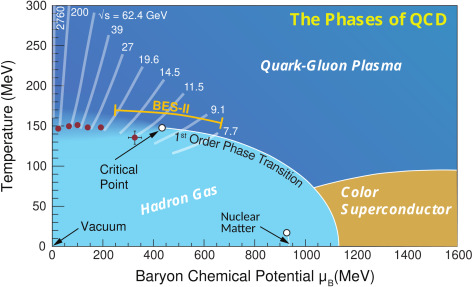
\includegraphics[width=0.5\linewidth]{images/1-s2.0-S0370157320300156-gr1.jpg}
    \caption{Фазовая диаграмма КХД-материи~\cite{Bzdak:2019pkr}.}
    \label{fig:qcd_phase_diagram}
\end{figure}

При больших температурах и низких бариохимических потенциалах, сильновзаимодействующая материя проявляет партонные степени свободы и характеризуется деконфайнментом кварков. 
Открытое в 2005 году на релятивистском ускорителе тяжелых RHIC~\cite{STAR:2005gfr}, это состояние получило название кварк-глюонной плазмы КГП.
Исследуя коллективные потоки, рожденных в столкновениях тяжелых ионов, было установлено, что эта форма материи обладает наименьшей известной в природе сдвиговой вязкостью.~\cite{Shen:2015msa}.
Вычисления КХД на решетке предсказывают плавный переход типа "crossover" от партонных степеней своды к адронным, при низких бариохимических потенциалах с уменьшением температуры~\cite{HotQCD:2014kol, Karsch:2003va}.
Экспериментальные доказательства этому были обнаружены в ходе первого скана по энергии на RHIC~\cite{Odyniec:2019kfh}.
Согласно современным представлениям, эпохе бариогенезиса предшествовало состояние горячей КГП с около нулевым барионным числом, которое завершилось плавным "crossover" переходом в состояние материи с преимущественно адронными степенями свободы~\cite{Esumi:2022uas}

При ненулевых бариохимических потенциалах, КХД-расчеты предсказывают переход первого рода из состояния с адронными степенями свободы в состояние с преимущественно кварковыми.
Существование двух видов фазового перехода: плавный типа "crossover" и перехода первого рода в одной области бариохимических потенциалов и температуры предполагает наличие критической точки~\cite{Odyniec:2019kfh}.
В области невысоких теператур и сверхвысоких бариохимических потенциалов теоретически предсказано существование еще более экзотической формы материи, такой как цвето-сверхпроводящая материя~\cite{McLerran:2008ux}.

В столкновениях тяжелых ионов при кинетических энергиях в несколько $A$~ГэВ образуется сильновзаимодействующая материя при температурах $T\approx150$~МэВ и чистых барионных плотностях в несколько раз превышающих плотность ядреной материи.
Исследование этой области фазовой диаграммы представляет интерес, поскольку предполагается, что такая материя встречается в компактных астрофизических объектах, к примеру, в нейтронных звёздах~\cite{Danielewicz:2002pu}.
Столкновениях ионов --- единственный способ лабораторно воссоздать условия, существующие в сложнонаблюдаемых космологических объектах.

Направленный и эллиптический потоки являются чувствительными наблюдаемыми к уравнению состояния, поскольку отражают изначальное распределение градиентов давления в системе.
Вычисления релятивистской гидродинамики предсказывают, что "смягчение" уравнения состояния должно сильно влиять на магнитуду и знак направленного потока протонов, что может являться сигналом фазового перехода первого рода при высоких барионных плотностях~\cite{Rischke:1995pe, Stoecker:2004qu}.
С ростом энергии и смягчении уравнения состояния, направленный поток должен менять знак с положительно на отрицательный.
Такая зависимость от энергии действительно наблюдалась в данных, опубликованных коллаборацией STAR~\cite{STAR:2014clz}.

\subsection{Описание динамики столкновения тяжелых ионов}


В результате столкновения тяжелых ионов в области перекрытия образуется сильно взаимодействующая материя, свойства которой сильно зависят от размера сталкивающихся ядер, и от энергии столкновения.
При столкновении тяжелых ядер, при энергиях в несколько ГэВ на нуклон налетающего ядра, время пролёта ионов сравнимо со временем существования материи в области перекрытия.
Процесс столкновения двух ядер можно условно разделить на несколько этапов.

При скоростях налетающего ядра, превышающих скорость звука в ядерной материи при обычных условиях ($\beta_S=0.2$)~\cite{Weber:1998aa}, нуклоны не могут покинуть область перекрытия достаточно быстро, и образуется зона высокой плотности.
В зависимости от уравнения состояния, которое связывает давление с плотностью и температурой, материя в зоне перекрытия может достигать условий, которые описываются средней плотностью и температурой.
В этих условиях могут быть созданы новые частицы, а их число и характер эмиссии могут быть использованы для исследования глобальных свойств вещества.
Отклонение плотным веществом в области перекрытия, остатков налетающего ядра с положительной быстротой происходит в направлении $+x$, что приводит к $\langle p_x \rangle  > 0$, а остатки ядра с отрицательной быстротой отклоняются в направлении $-x$, имея $\langle p_x \rangle < 0$.
Таким образом, направленный поток остатков налетающего ядра является положительным для частиц с положительной бысротой и отрицательным для частиц с отрицательной быстротой.
Измерения направленного потока частиц, относительно плоскости симметрии определенной спектаторами даёт информацию о времени взаимодействия рожденных частиц с областью перекрытия.
Положительный направленный поток частиц относительно плоскости симметрии остатков налетающего ядра говорит о довольно большом времени взаимодействия, при котором материя в области перекрытия успевает смешаться с холодной спектаторной материей.
Эллиптический поток $v_2$ несёт информацию о давлении в области перектия сталкивающихся ионов.
При энергиях порядка 1~ГэВ, значения $v_2$ отрицательные относительно плоскости симметрии спектаторов.
Остатки сталкивающихся ядер блокируют вылет частиц в плоскости реакции, что ведет к вылету частиц перпендикулярно плоскости реакции.
Чем выше давление, достигаемое в области перекрытия, тем выше будут значения $v_2$.
Схематически эти механизмы изображены на рис.~\ref{fig:bounce_off}.
%
\begin{figure}[ht]
\begin{center}
    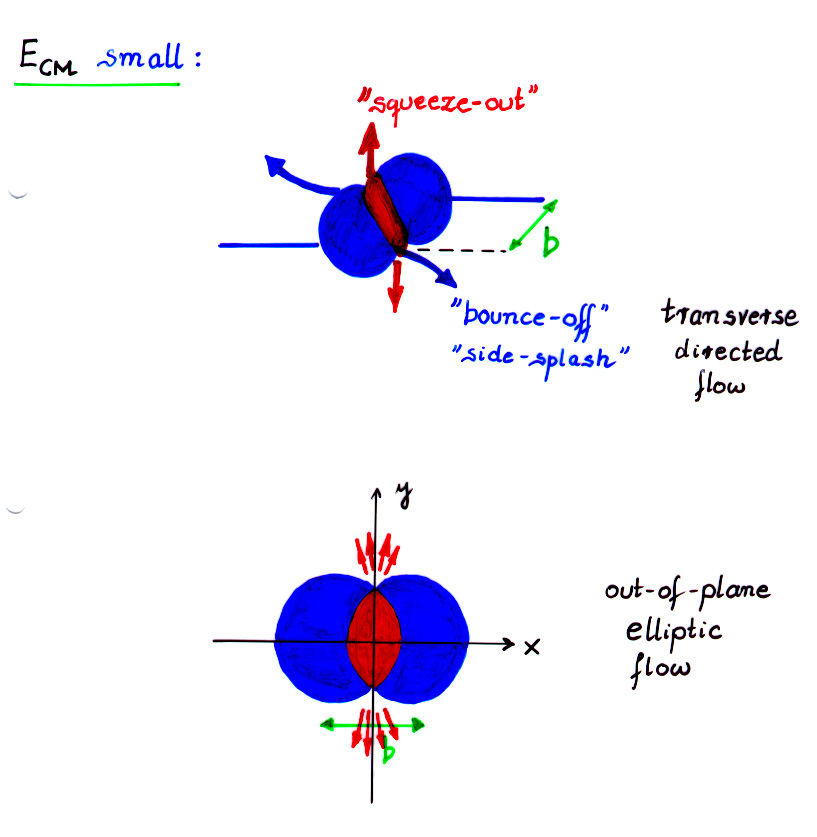
\includegraphics[width=0.75\linewidth]{images/bounce_off.jpg}
    \caption{Схематичное изображение механизмов рождения направленного (bounce-off) эллиптического (squeeze-out) потоков.}
    \label{fig:bounce_off}
\end{center}
\end{figure}
%

Партисипанты, или нуклоны сталкиващихся ядер, претерпевают многократные рассеяния.
В результате рождаются новые частицы и изменяются импульсы частиц, составляющих материю в области перекрытия.
Если время взаимодействия достаточно велико, то материю в области перекрытия можно описать при помощи статистических величин: средняя плотность, средняя температура и т.д..
При многократном рассеянии частиц, составляющих материю в области перекрытия, может происходить подпороговое рождение частиц.
Сравнивая коллективные потоки различных типов частиц, рожденных в области перекрытия можно судить о степени термализации или релаксации энергии в области перекрытия.
Чем ближе потоки различных типов сталкивающихся частиц к среднему значению, тем больше степень термализации материи.
По степени термализации можно судить о времени существования материии в области перекрытия.  

Реакция и развитие коллективных эффектов останавливаются на стадии столкновения, обычно называемой фриз-аут. 
В этой фазе плотности достаточно малы, чтобы в течение типичной длины пролета больше не происходило взаимодействия.
Хотя многие наблюдаемые (например, спектры рожденных частиц) теряют память о начальных условиях во время процесса эволюции, ожидается, что коллективные потоки адронов несут информацию о самых ранних этапах столкновения~\cite{Herrmann:1999wu}.
Коллективные потоки рожденных адронов сильно зависят от начальной геометрии столкновения.
Коллективное движение рожденых адронов обусловлено взаимодействием частиц составляющих материю в области перекрытия.
Характер этого взаимодействия обусловлен свойствами материи, которые описываются уравнением состояния.
Поэтому зная изначальную геометрию столкновения, которая определяется центральностью и измеряя итоговую анизотропию рожденных частиц можно извлечь уравнение состояния сильновзаимодействующей материи.

Коллективное движение частиц приводит к корреляции импульсов рожденных адронов.
Таким образом, изучая эту корреляцию, можно количественно оценить коллективные эффекты.
Однако это не единственный канал, по которому импульсы рожденных частиц могут быть скоррелированы.
К примеру, импульсы частиц, рожденных в слабом или сильном распаде резонанса относятся следующим образом:
%
\begin{equation}
    P = P_1 + P_2,
\end{equation}
где $P$ --- 4-импульс резонанса, $P_{1,2}$ --- импульсы рожденных в распаде частиц.
Также в силу сохранения поперечного (полного) импульса системы справедливо следующее соотношение:
%
\begin{equation}
    \sum_{k=1}^{N} \vec{p_T}^k = 0,
\end{equation}
где $N$ --- множественность рожденных частиц, $\vec{p_{T}}^k$ --- поперечный импульс $k$-й частицы.
Корреляция импульсов частиц, рожденной в бинарном столкновении частиц, составляющих материю тоже подчиняется законам сохранения импульса:
%
\begin{equation}
    P_1 + P_2 = P_3 + P_4 + P_5.
\end{equation}

Описанные выше эффекты не имеют отношения к коллективному движению частиц, однако обеспечивают корреляцию импульсов.
Такие эффекты носят название непотоковых корреляций и осложняют измерение коллективных эффектов.
Поэтому для подавления непотоковых эффектов чаще всего рассматривается корреляция большого колличества частиц.
Также для подавления корреляций не связанных с коллективным движением частиц можно рассматривать корреляцию областей со значительнми разделением по кинематике.
Оценка вклада остаточных непотоковых корреляций является важной задачей при измерении коллективных эффектов.

\subsection{Определение уравнения состояния сильновзаимодействующей материи}

Уравнение состояния сильновзаимодействующей материи можно восстановить путём сравнения экспериментально наблюдаемых сигналов, доступных из столкновения тяжелых ионов (таких как выходы частиц, их импульсные спектры, коллективная анизотропия рожденных частиц) с предсказаниями теоретических моделей с различными EOS.
Прямые вычисления КХД возможны лишь при нулевых бариохимических потенциалах и в области больших чистых барионных плотностей неприменимы.
Поэтому теоретические модели в области низких энергий столкновений ограничены описанием динамики системы.
Можно выделить два вида динамических моделей: релятивистская гидродинамика~\cite{Stoecker:1986ci,Hung:1994eq,Werner:2010aa} и транспортные модели, основанные на релятивистском транспортном уравнении Больцмана~\cite{Molnar:2004yh,Xu:2004mz}.

Первый подход основан на приближении, что образованная система может быть описана как расширяющаяся жидкость, достигшая локального термодинамического равновесия. 
Основное преимущество такого подхода заключается в довольно лёгкой интерпретации уравнения состояния системы, которое вычисляется в термодинамическом подходе~\cite{Stoecker:1986ci}.
Основная проблема релятивистской гидродинамики заключается в предположении, что система успевает достичь термодинамического равновесия, что может быть неверно.

Транспортные модели лишены этого недостатка, поскольку описывают процесс столкновения ядер через многократные упругие и неупругие рассеяния адронов.
Наличие или отсутствие локального равновесия не влияет на решение релятивистского транспортного уравнения Больцмана.
Недостатком же такого подхода является то, что он основан на предположении, что многочастичные рассеяния можно свести к двухчастичным.
До сих пор, справедливо ли это предположение, не доказано.
Более того, для моделирования каждого вида рассеяния необходимо обладать значениями сечений взаимодействий, которые для тяжелых резонансов остаются свободными параметрами модели.
Имплементация уравнения состояния системы часто выполняется путём варьирования среднего потенциала взаимодействия~\cite{Nara:2016hbg}.

Транспортные модели описывают распространение частиц в образованной материи при помощи одночастичного потенциала $U(\rho, p)$, где $\rho$ и $p$ --- плотность материи достигнутая в столкновении и импульс частицы.
Этот потенциал в простейшем виде можно выразить в виде параметризации Скёрма без импульсной зависимости:
\begin{equation}
    U(\rho) = a(\rho/\rho_0) + b(\rho/\rho_0)^\sigma
    \label{eq:skyrme}
\end{equation}
Параметры $a$, $b$ и $\sigma$ подбираются таким образом, чтобы отвечать свойствам системы: энергия связи на нуклон плотность насыщения и несжимаемость материи K.
Несжимаемость материи в ядерной физике определяется следующим образом:
\begin{equation}
    K = R^2 \frac{d^2 e/\rho}{ d^2 R },
\end{equation}
где вторая производная берётся в предположении постоянного числа нуклонов и энтропии, $e$ --- плотность энергии и $R$ --- радиус ядра.
Предполагается, что коллективное расширение области перекрытия чувствительно к коэффициенту несжимаемости материи $K$.

Сравнение теоретических предсказаний с потенциалом~(\ref{eq:skyrme}) для среднего импульса $\langle p_x / A \rangle$ с экспериментальными данными показывает лучшее согласие для очень больших значений $K \ge 380$~MeV~\cite{Kruse:1985hy, Molitoris:1985gs}.
В то же самое время феноменологический подход с импульсно-зависимым потенциалом, описанный в~\cite{Gale:1987zz, Aichelin:1987ti, Welke:1988zz, Haddad:1995vt} показывает хорошее согласие с данными при относительно небольшой несжимаемости $K=215$~МэВ.
Хотя теоретические модели с импульсно-зависимым потенциалом $U(\rho, p)$ довольно хорошо описывают равновесные свойства ядерной материи, они могут довольно сильно различаться между собой в неравновесной фазе столкновения, которая доминирует в начальные моменты реакции.
Это может влиять на более поздние этапы столкновения и приводить к различной достигнутой плотности.

При таком динамическом подходе, параметры уравнения состояния ядерной материи быстро меняются со временем, а все наблюдаемые являются наблюдаемыми конечного состояния. 
Экспериментально недоступны ни начальное ни промежуточные состояния. 
При энергиях столкновения $E_{kin}<10A$~ГэВ время расширения материи в области перекрытия, которое определяется скоростью звука, сравнимо со временем пролёта сталкивающихся ядер.
Поэтому спектаторы --- остатки сталкивающихся ядер --- блокируют вылет рожденных частиц в плоскости реакции, что приводит к отрицательному $v_2$ рожденных частиц. 
Смешивание холодной спектаторной и горячей, рожденной в столкновении материй и расширение этой материи приводят к положительным значениям $v_1$ протонов.
Уменьшение времени пролёта при увеличении энергии столкновения, приводит к спаду магнитуды направленного и эллиптического потоков. 
С ростом энергии эллиптический поток меняет знак с отрицательного на положительный, что свидетельствует о преимущественном вылете частиц в плоскости реакции.
Система, образованная в столкновения тяжелых ионов в данной области энергии характеризуется сложной геометрией из-за присутствия спектаторов.
Изучение зависимости коллективных потоков от геометрии столкновения и размеров системы может пролить свет на свойства созданной в столкновении материи.

Экспериментальные измерения направленного потока протонов в диапазоне энергий 2-10$A$~Гэв были выполнены коллаборацией E895 на ускорителе AGS в Национальной Лаборатории в Брукхевене~\cite{E895:2000maf}. 
Теоретический анализ этих измерений был выполнен Данилевичем, Лейси и Линчем в 2002 году~\cite{Danielewicz:2002pu}.
Экспериментальные данные для наклона бокового потока и эллиптического потока были сопоставлены с теоретическими предсказаниями для различных коэффициентов несжимаемости материи $K$.
Сравнение показано на рис.~\ref{fig:Danilewicz}. 
Экспериментальные данные позволили отсечь лишь экстремальные значения коэффициента несжимаемости $K$.
Значения для наклона бокового потока $F$ лучше согласуются с теоретическими предсказаниями с $K=210$~МэВ. 
Данные для эллиптического потока лучше описываются более жестким уравнением состояния с $K=300$~МэВ.
Это несоответствие может быть вызвано вкладом корреляций, не связанных с коллективным движением рожденных адронов (непотоковые корреляции).
Новые экспериментальные данные, выполненные методами, позволяющими учесть вклад непотоковых корреляций позволят разрешить эту неоднозначность полученных значений $K$.

\begin{figure}[h]
    \centering
    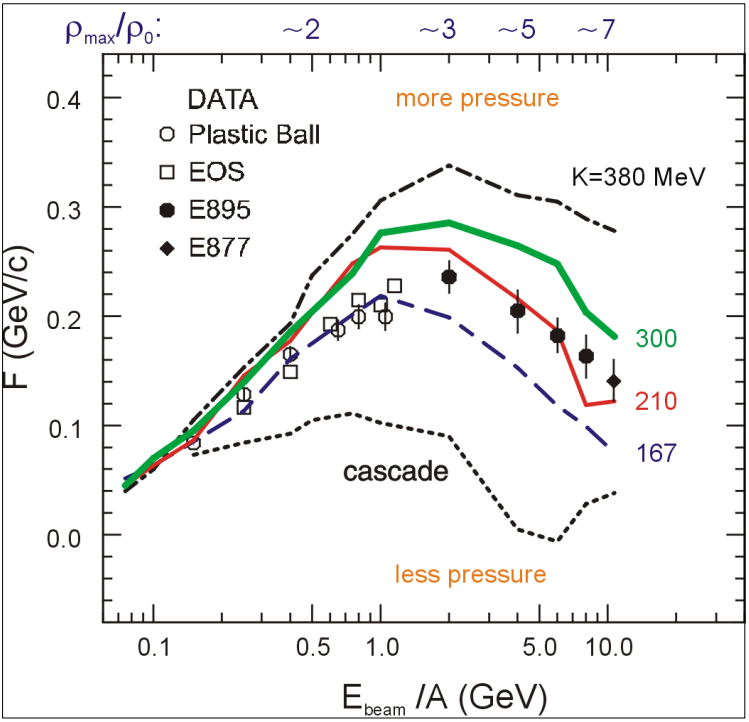
\includegraphics[width=0.45\linewidth]{images/Danilewicz_F_energy.png}
    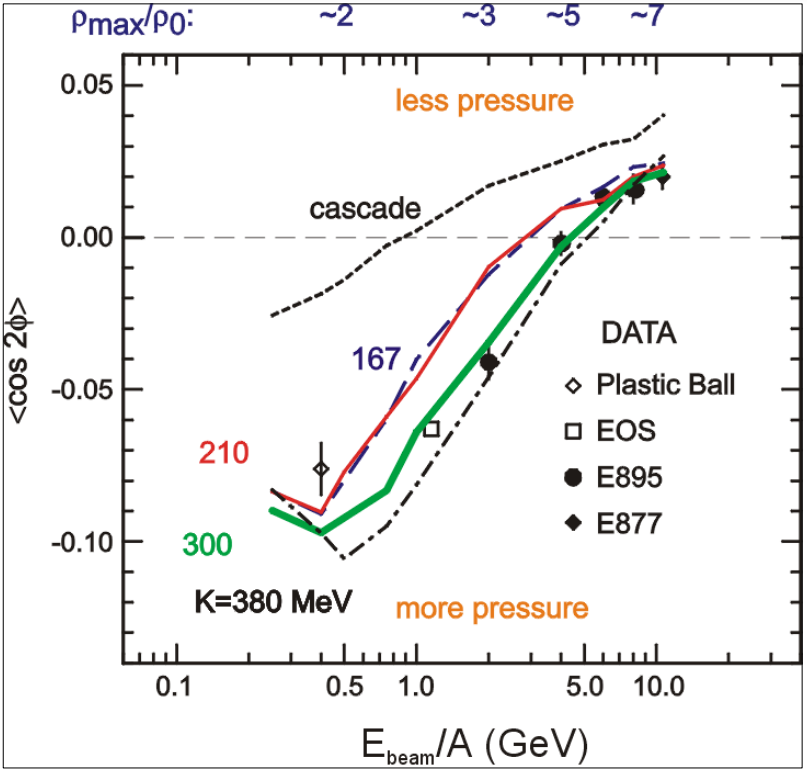
\includegraphics[width=0.45\linewidth]{images/Danilewicz_Elliptic_energy.png}
    \caption{Сравнение данных для наклона бокового потока (слева) и эллиптического потока (справа) как функция энергии с теоретическими расчетами для разных значений коэффициента несжимаемости~\cite{Danielewicz:2002pu}.}
    \label{fig:Danilewicz}
\end{figure}

На рис.~\ref{fig:dv1dy_energy} представлена зависимость наклона направленного потока протонов $dv_1/dy|_{y=0}$ от энергии столкновения ядер золота.
На рисунке показаны данные с экспериментов FOPI~\cite{FOPI:2011aa} и предварительные данные эксперимента STAR Fixed Target.
Наблюдается монотонное уменьшение наклона с ростом энергии.
Новые экспериментальные измерения направленного потока позволят дополнить существующие мировые данные по коллективным потокам протонов в области энергии в несколько $A$~ГэВ.
%
\begin{figure}
    \centering
    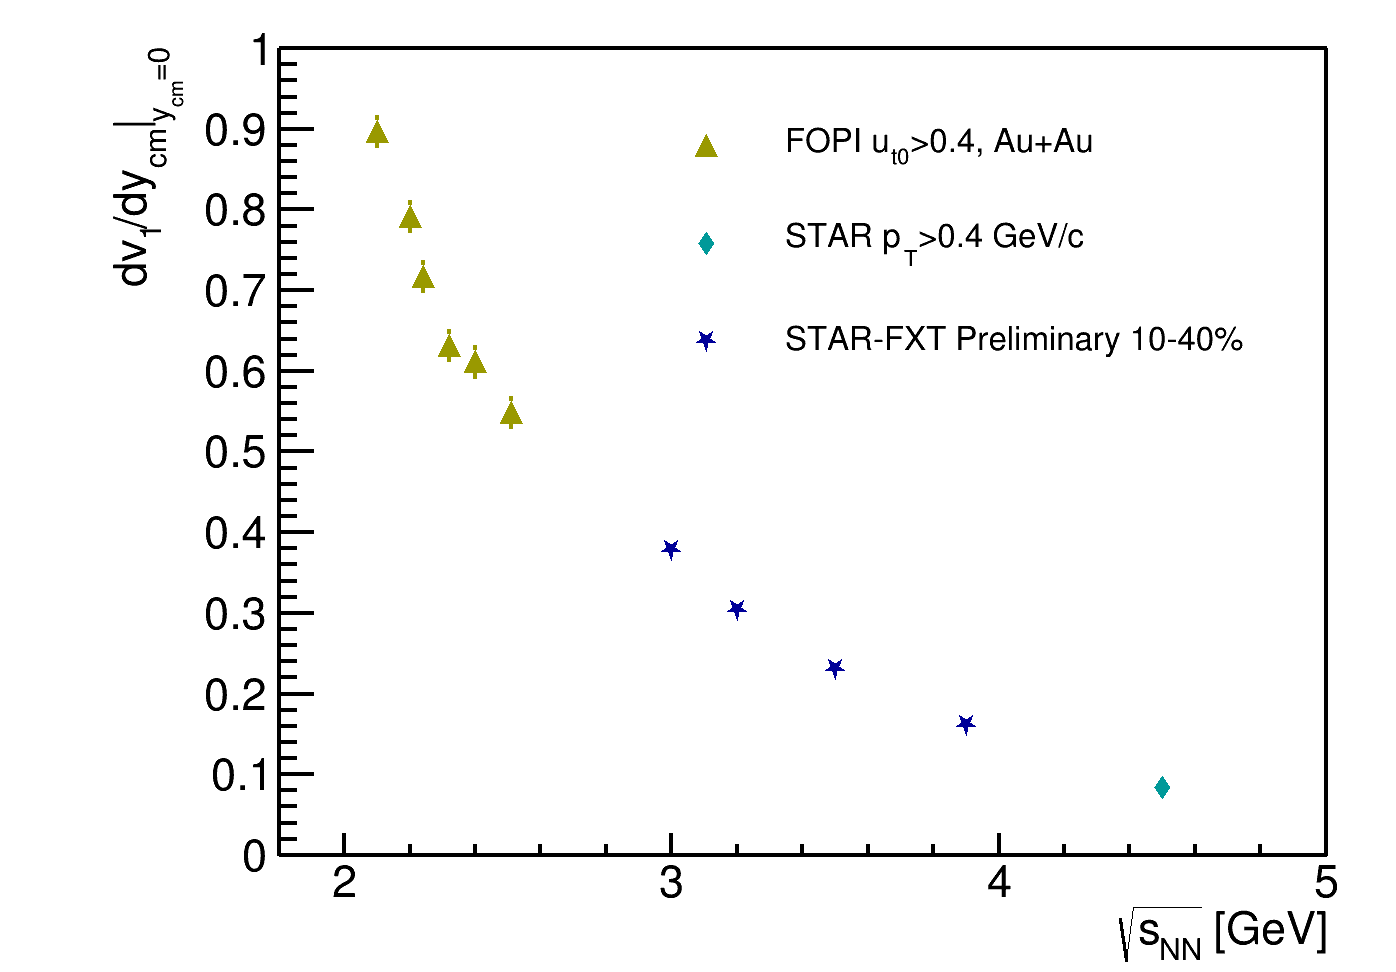
\includegraphics[width=0.5\linewidth]{images/dv1dy_sqrt_snn.png}
    \caption{Зависимость наклона направленного потока протонов $dv_1/dy|_{y=0}$ от энергии столкновения ядер золота.}
    \label{fig:dv1dy_energy}
\end{figure}

\section{Основные определения}

\subsection{Центральность столкновения}
\label{theory:centrality}
Наблюдаемые, чувствительные к свойствам созданной в области перекрытия материи, зависят от геометрии столкновения~\cite{ALICE:2010mlf,ALICE:2015juo}.
Геометрия столкновения может быть описана при помощи таких переменных, как прицельный параметр столкновения $b$, число бинарных нуклон-нуклонных столкновений $N_{col}$ и число нуклонов-участников взаимодействия $N_{part}$.
Для того, чтобы характеризовать геометрию столкновения наименее зависящим от экспериментальной установки методом, была введена такая величина, как центральность столкновения $C_b$.
Центральность столкновения определяется как доля полного сечения взаимодействия сталкивающихся ядер $\sigma_{inel}^{AA}$ при данном значении прицельного параметра $b$:
\begin{equation}
    C_b = \frac{1}{\sigma_{inel}^{AA}} \int_{0}^{b} \frac{d\sigma}{db'}db',
\end{equation}
где $d\sigma/db$ --- дифференциальное сечение взаимодействия ядер.

Прицельный параметр $b$ не может быть измерен, поэтому для определения центральности в условиях эксперимента используются скоррелированные с ним величины, такие как например множественность рожденных частиц~\cite{Segal:2020ftt,HADES:2017def}.
Центральность по множественности столкновения определяется формулой:
\begin{equation}
    C_M = \frac{1}{\sigma_{inel}^{AA}} \int_{M}^{\infty} \frac{d\sigma}{dM'}dM',
\end{equation}
где $M$ --- множественность зарегистрированных рожденных частиц.

Столкновения ионов группируются в классы центральности, согласно множественности рожденных частиц.
Поскольку в распределении прицельного параметра и числа рожденных частиц, наблюдается не нулевая ширина, определеные классы центральности по множественности лишь в среднем совпадают с определенными по прицельному параметру.
События с классом центральности 0\% отвечают наиболее центральным столкновениям и 100\% --- наиболее переферическим.

Для вычисления значений прицельного параметра (или других геометрических параметров) в определенных по множественности классах центральности, часто использутся модель Монте-Карло Глаубера~\cite{Miller:2007ri}.
Модель Монте-Карло Глаубера описывает столкновения ядер следующим образом:
\begin{itemize}
    \item Столкновения ионов рассматривается как последовательность независимых нуклон-нуклонных столкновений, вероятность которых определятся сечением неупругих нуклон-нуклонных рассеяний.
    \item Изначальное распределение нуклонв в ядре разыгрывается при помощи метода Монте-Карло согласно распределению Вудса-Саксона ядерной плоности:
    \begin{equation}
        \rho(r) = \frac{ \rho_0 }{ 1 + e^{ (r-R)/a } },
        \label{ eq:woods_saxon }
    \end{equation}
    где $\rho_0$ --- нормировочный коэффициент, $r$ --- расстояние от центра ядра, $R$ --- радиус ядра и $a$ --- параметр толщины оболочки.
    Данные параметры подбираются для каждого ядра и каждой энергии столкновения.
    \item Каждый нуклон движется по прямолинейной траектории во время процесса столкновения.
\end{itemize}

Множественность столкновения моделируется при помощи геометрических параметров ($N_{part}$, $N_{col}$), разыгранных в модели МК-Глаубера.
Суммарная множественность набирается из множественности частиц, рожденных в каждом единичном источнике $a$: $M=\sum_{a=1}^{N_a} M_a$, где $N_a$ --- число источников.
Число источников определятся формулой, которая моделирует жесткие процессы через зависимость от $N_{col}$ и мягкие процессы через зависимость от $N_{part}$:
\begin{equation}
    N_a = f N_{part} + (1-f) N_{col}.
\end{equation}

Для каждого источника $a$ число рожденных частиц $M_a$ разыгрывается при помощи отрицательного биномиального распределения с параметрами $\mu$ --- среднее и $k$ --- ширина:
\begin{equation}
    P_{\mu,k}(n) = \frac{ \Gamma (n+k) }{ \Gamma(n+1) \Gamma(k) } \frac{ (\mu/k)^n }{ (\mu/k+1)^{n+k} },
\end{equation}
где $P_{\mu,k}(n)$ --- вероятность источника родить $n$ частиц.

В дальнейшем параметры $f$, $\mu$ и $k$ подбираются таким образом, чтобы разыгранная множественность наилучшим образом описывала экспериментальное распределение множественности.

\subsection{Вектора потоков $u_n$ и $Q_n$}

Методы измерения коллективных потоков довольно просто описать в терминах векторов.
Для измерения азимутальных потоков каждой частице ставится в соответствие единичный вектор $u_n$ в плоскости перпендикулярной оси пучка на основании импульса частицы:
%
\begin{equation}
    \vec{u}_n = (x_n, y_n) = ( \cos n \varphi, \sin n \varphi ),
\end{equation}
%
где $\varphi$ --- азимутальный угол частицы, $n$ --- порядок гармоники. 
При очень большом количестве частиц в одном событии ($N \gg 1$), сумму по всем частицам можно заменить на интеграл (аналогично, при небольшой множественности частиц и большом числе событий, можно рассматривать все события с выбранной плоскостью реакции $\Psi^R$):
%
\begin{equation}
    \sum_{k=1}^{N} \vec{u}_n = \int_{-\pi}^{\pi} \vec{u}_n(\phi) \rho(\phi-\Psi^R) d\phi
\end{equation}
Рассмотрим интеграл по $x$-компоненте $u_n$ вектора:
%
\begin{equation}
    \int_{-\pi}^{\pi} x_n \rho(\phi-\Psi^R) d\phi =
    \int_{-\pi}^{\pi} \cos n ( \phi - \Psi^R + \Psi^R ) \rho(\phi - \Psi^R) = V_n \cos (n\Psi^R), 
\end{equation}
где $V_n$ пропорционален множественности частиц $N$ и значению $v_n$ для данной группы частиц в данном событии.
Аналогичные преобразования можно выполнить и для $y$-компоненты $u_n$-вектора, получив $V_n\sin(n\Psi^R)$.
Таким образом, сумма $u_n$-векторов в одном событии даёт оценку плоскости реакции события.

Эта оцнека, определяемая суммой единичных векторов частиц носит название $Q_n$-вектора:
%
\begin{equation}
    \vec{Q}_n = \frac{1}{C} \sum_{k=1}^{N} w_k u_n^k = \frac{|Q_n|}{C} (\cos{(n\Psi_n)}, \sin{(n\Psi_n)}),
    \label{eq:track_qn}
\end{equation}
%
где $k$ --- индекс частицы в группе, $w_k$ --- вес $k$-го вектора, $N$ --- множественность частиц в группе, $\Psi_n$ --- угол плоскости симметрии данного события и данной гармоники $n$, $|Q_n|$ --- модуь $Q_n$-вектора и $C$ --- нормировочный коэффициент. 
Чем больше число частиц в событии $N$, тем ближе оценка угла плоскости симметрии к реальной ориентации плоскости реакции:
%
\begin{equation}
    \lim_{N \xrightarrow{} \infty} \frac{1}{C} \sum_{k=1}^{N} w_k u_n^k = \frac{|Q_n|}{C} (\cos (n\Psi^R), \sin (n\Psi^R) ) .
\end{equation}

\section{Методы измерения коллективной анизотропии в столкновениях тяжелых ионов}

\subsection{Методы плоскости события и скалярного произведеления}

Выбор значения нормировочного коэффициента определяет метод измерения направленного потока. 
В работе исследуются два метода: плоскости события (EP) и скалярного произведения (SP)~\cite{Mamaev:2020lpi}. 

Метод плоскости события требует такую нормировку, чтобы модуль каждого $Q_1$-вектора был равен 1, что соответствует $C=|Q_n|$. 
В работах~\cite{Borghini:2001vi, Bhalerao:2006tp} было показано, что в таком случае, измеренное значение потока $v_n\{EP\}$ нелинейно зависит от множественности частиц, использованных для вычисления $Q_n$-вектора, а также от значения самого потока. 
В пределе большого количества частиц и большого значения потока ($v_n \sqrt{M} \gg 1$), измеренные значения стремятся к среднему значению $v_n$: $v_n\{EP\} \xrightarrow{} \langle v_n \rangle$. 
В случае малого числа частиц, использованных для построения $Q_n$-вектора, а также малых значениях потока ($v_n \sqrt{M} \ll 1$), измерения стремятся к корню среднего квадрата $ v_n\{EP\} \xrightarrow{} \sqrt{ \langle v_n^2 \rangle }$.
Экспериментально измеренные значения $v_1\{EP\}$ находятся между двумя пределами: $ \langle v_n \rangle \leq v_n\{EP\} \leq \sqrt{ \langle v_n^2 \rangle } $.
В зависимости от реального значения $v_n$ (который определяется энергией столкновения и размером сталкивающихся ядер) и множественности частиц (которая зависит от энергии, размера ядер и аксептанса установки), измеренные значения $v_n\{EP\}$ могут лежать ближе к правому или левому пределам.

Второй метод, скалярного произведения (SP), требует нормировку на сумму весов $C=\sum_{k=1}^N w_k$.
Модуль $Q_n$-вектора сохраняет информацию о множественности частиц, использованных для его построения, а также их $v_n$: $|Q_n| \propto v_n M$.
Использование такой нормировки дает значения $v_n\{SP\} \xrightarrow{} \sqrt{\langle v_n^2 \rangle}$ независимо от измеренной множественности частиц, а также их $v_n$.

Несмотря на известные недостатки метода плоскости события, он до сих пор активно используется, поскольку более прост в реализации. 
В частности, измерения коэффициентов коллективных потоков $v_n$ в коллаборации HADES~\cite{HADES:2020lob} были выполнены методом плоскости события. 
В работе была произведена оценка систематической ошибки на измереные $v_n$, путём сравнения результатов полученных методами скалярного произведения и плоскости события~\cite{Mamaev:2020lpi}.

\subsection{Разрешение плоскости симметрии}

Экспериментально направленный поток можно определить как проекцию $u_n$-вектора частиц на плоскость симметрии события:
%
\begin{equation}
    v_n' =  \langle u_n Q_n \rangle = 
    V_n \langle \cos (n\phi) \cos (n\Psi_n) \rangle + V_n \langle \sin(n\phi) \sin(n\Psi_n) \rangle,
\end{equation}
%
где диагональные члены равны нулю в силу симметрии столкновения относительно плоскости реакции, а коэффициент $V_n$ появляется после усреднения модулей вектора $Q_n$.
Раскрывая тригонометрические выражения в угловых скобках, можно получить:
%
\begin{equation}
\begin{align}
    \langle \cos (n\phi) \cos (n\Psi_n) \rangle = \langle \cos n ( \phi - \Psi_n ) \rangle = 
    = \langle \cos n ( \phi - \Psi_n + \Psi^R - \Psi^R ) \rangle = \\
    \langle \cos n ( \phi - \Psi^R ) \cos n (\Psi_n - \Psi^R ) \rangle
\end{align}
\end{equation}
%
Аналогичные преобразования можно выполнить и для синусов. 
Измеренные значения направленного потока имеют вид:
%
\begin{equation}
    v_n' =  \langle u_n Q_n \rangle = 
    V_n \langle \cos n ( \phi - \Psi_n ) \cos n (\Psi_n - \Psi^R) \rangle.
    \label{eq:uq_transformation}
\end{equation}
%

Поскольку вычисленная плоскость симметрии столкновения $\Psi_n$ лишь приблизительно описывает ориентацию плоскости реакции $\Psi^R$, значение $ \langle \cos(\Psi_n - \Psi^R) \rangle \ne 1 $.
Флуктуации распределения энергии в сталкивающихся ядрах приводят к флуктуации плоскости симметрии относительно плоскости реакции реакции, как показано на рис.~\ref{fig:pp_sp_rp}
Поэтому измеренные значения $v_n'$ будут отличаться от действительных.
Для коррекции этого этого эффекта, необходимо ввести поправочный коэффициент разрешения:
%
\begin{equation}
    R_n = V_n \langle \cos n (\Psi_n - \Psi^R) \rangle.
\end{equation}
%

%
\begin{figure}[ht]
\begin{center}
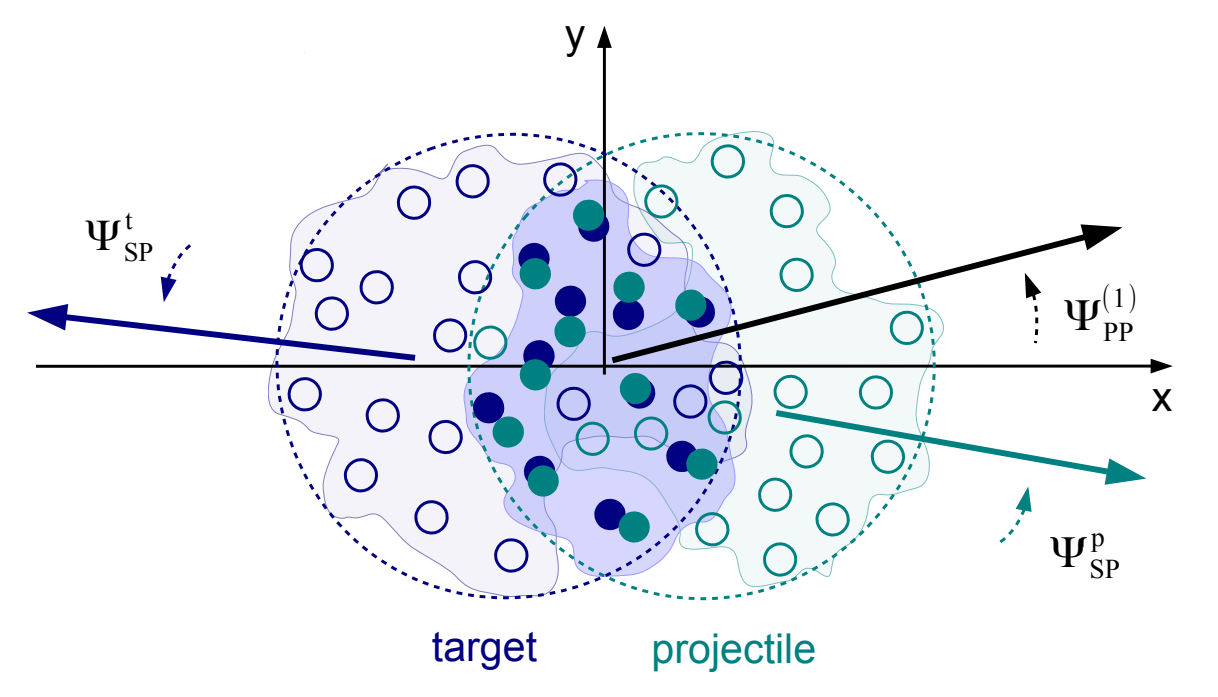
\includegraphics[width=0.75\linewidth]{images/v1_pp_sp.png}
\caption{Схематическое представление сталкивающихся ядера в плоскости перпендикулярной направлению пучка.}
\label{fig:pp_sp_rp}
\end{center}
\end{figure}
%

Скорректированные на разрешение значения $v_1$ могут быть записаны следующим образом: 
%
\begin{equation}
    v_n =  \frac{ \langle u_n Q_n \rangle }{R_n},
    \label{eq:v1_formula}
\end{equation}
%

\subsection{Метод случайных подсобытий}

Для вычисления $R_n$ в эксперименте, можно воспользоваться попарными корреляциями $Q_n$-векторов (преобразование выполнено аналогично уравнению (\ref{eq:uq_transformation})): 
%
\begin{equation}
    \langle Q_n^a Q_n^b \rangle = V^a_n V^b_n \langle \cos n (\Psi^a_n - \Psi^R) \cos(\Psi^b_n - \Psi^R) \rangle,
\end{equation}
%
где индексами $a$ и $b$ обозначены две различных группы частиц, в каждой из которых $Q_n$-вектор вычислялся независимо.

Наиболее простым методом вычисления разрешения является метод двух подсобытий:
%
\begin{equation}
    R_n\{a,b\} = \sqrt{ \langle Q_n^a Q_n^b \rangle } = \sqrt{ V_n^2 \langle \cos^{2}( \Psi^{a,b}_n - \Psi_R ) \rangle },
    \label{eq:r1_2sub}
\end{equation}
где индексами $a$ и $b$ обозначены две группы частиц, идентичные по множественности и значению $v_n$, в которых $Q_n$-вектор вычислялся независимо.
В коллайдерных экспериментах, где аксептанс часто симметричен относительно средних быстрот, в качестве подсобытий $a$ и $b$ могут быть выбраны частицы в диапазонах по быстроте, симметричных относительно нуля.
В экспериментах с фиксированной мишенью, где такое выполнить невозможно в силу несимметричного аксептанса, иногда пользуются методом, называемым метод случайных подсобытий.
Подсобытия $a$ и $b$ набираются случайным образом из частиц в выбранном кинематическом окне.
Этот метод прост в исполнении, однако корреляция $Q_1$-векторов из одной кинематической области может быть подвержена довольно большому вкладу непотоковых корреляций~\cite{Mamaev:2020lpi}.
Экспериментальные значения $v_n$, полученные коллаборацией HADES~\cite{HADES:2020lob} измерены, испльзуя метод случайных подсобытий для коррекции на разрешение плоскости симметрии. 
Вычисляя $R_n$ отличным от использованного коллаборацией HADES методом, предлагается оценить вклад непотоковых корреляций в измерененные значения $v_n$~\cite{Mamaev:2020lpi, Mamaev:2020qom}.

\subsection{Метод трех подсобытий}

Комбинируя различные попарные корреляции векторов, можно вычислить разрешение плоскости симметрии для данного $Q_n$-вектора:
%
\begin{equation}
    R_n\{a(b,c)\}  =  \sqrt { \frac{ \langle Q_n^a Q_n^b \rangle \langle Q_n^a Q_n^c \rangle }{ \langle Q_n^b Q_n^c \rangle} },
    \label{eq:r1_3sub}
\end{equation}
%
где $a$, $b$ и $c$ --- три различных группы частиц, в каждой из которых $Q_1$-вектор вычислялся независимо.
Этот метод вычисления $R_n$ носит название метод трёх подсобытий.
Метод трёх подсобытий не накладывает ограничений на множественность частиц в каждой группе, что даёт большую свободу в выборе кинематических диапазонов для определения $Q_n$.
Корреляции $Q_n$, рассчитанных в близких кинематических диапазонах, всё еще могут быть подвержены непотоковым эффектам.
Это может приводить к неверному рассчету значений поправочного коэффициента $R_n$.
Автором предлагается исследовать связанную с этим систематическую ошибку путем сравнения $R_n$, полученнного с использованием различных комбинаций $Q_1$ (к примеру $R_1\{a(b,c)\}$ и $R_1\{a(b,d)\}$).
Эффекты не связанные с коллективным движением частиц могут вносить вклад в корреляцию между $u_n$-векторами частиц и $Q_n$-векторами плоскости симметрии.
Сравнивая $v_n$, полученные относительно различных плоскостей симметрии (к примеру, $v_n\{a\}$ и $v_n\{b\}$), предлагается вычислить вклад непотоковых корреляций в результаты для коллективного потока~\cite{Mamaev:2020qom,Mamaev:2023fpr,Mamaev:2023yhz,Mamaev:2024}. 

\section{Эффекты, необходимые учитывать при измерени коллективной анизотропии}

\subsection{Влияние эффективности на измеренный $v_n$}

Коллективная анизотропия рожденных в столкновении частиц обычно измеряется дифференциально как функция центральности, поперечного импульса и быстроты.
Неоднородная эффективность детектора в зависимости от этих переменных может приводить к неправильным значениям потоков при усреднении по этим переменным.
К примеру, при усреднении коэффициентов потока по поперечному импульсу в границах $p_T^{1,2}$ вклад неоднородной эффективность детектора $e(p_T)$ можно выразить следующим образом:
\begin{equation}
    v_n(p_T^1, p_T^2) = \int_{p_T^2}^{p_T^2} dp_T \frac{dN}{dp_T} e(p_T) v_n(p_T),
\end{equation}
где $\frac{dN}{dp_T}$ --- распределение частиц по поперечному импульсу.
Измеренные значения $v_n(p_T^1, p_T^2)$ будут отличаться от настоящего среднего в данном диапазоне импульсов.

Для коррекции на этот эффект, обычно вычисляется карта эффективности $e(p_T, y)$ установки при помощи Монте-Карло моделирования отклика детектора.
И усреднение по поперечному импульсу и быстроте выполняется с весом, обратным эффективности $1/e(p_T, y)$.

\subsection{Влияние азимутальной неоднородности аксептанса детектора}

Значительный вклад в результаты измерения азимутальных потоков может вносить неоднородность аксептанса детектора. 
Азимутальная анизотропия аксептанса искажает распределение $u_n$  и $Q_n$-векторов, которые в идеальном случае должны быть равномерными. 
Для коррекции этого эффекта был использован метод, описаный в работе~\cite{Selyuzhenkov:2007zi}.
Поскольку плоскость реакции распределена равномерно, в пределах большого количества столкновений формулу~(\ref{eq:v1_formula}) можно преобразовать следующим образом:
%
\begin{equation}
    v_n =  2\frac{ \langle x_n X_n \rangle }{R_n^X} = 2\frac{ \langle y_n Y_n \rangle }{R_n^Y},
    \label{eq:v1_formula}
\end{equation}
%
где $x_n$ и $y_n$ --- компоненты $u_n$-вектора, $X_n$ и $Y_n$ --- компоненты $Q_n$-вектора и $R_n^{X,Y}$ --- разрешение плоскости симметрии, вычисленное при помощи корреляций компонент $Q_n$-векторов.
Азимутальная неоднородность детектора нарушает это равенство.

Основные эффекты, вызываемые неоднородностью аксептанса могут быть выражены в следующем:
\begin{enumerate}
    \item Сдвиг $u_1$ ($Q_1$) вектора из-за ненулевых средних значений компонент:
    \begin{equation}
        \langle x_1 \rangle \ne 0, \langle y_1 \rangle \ne 0
    \end{equation}
    Коррекция на этот эффект носит название перецентровки.
    \item Поворот $u_1$ ($Q_1$) векторов. Коррекция на этот эффект называется коррекцией поворота
    \item Сужение/Расширение распределения компонент $u_1$ ($Q_1$) вектора. Коррекция носит название ремасштабирования.
\end{enumerate}
Схематическое представление эффекта применения коррекций представлено на рис.~\ref{fig:qn_corrections}.

\begin{figure}[h]
    \centering
    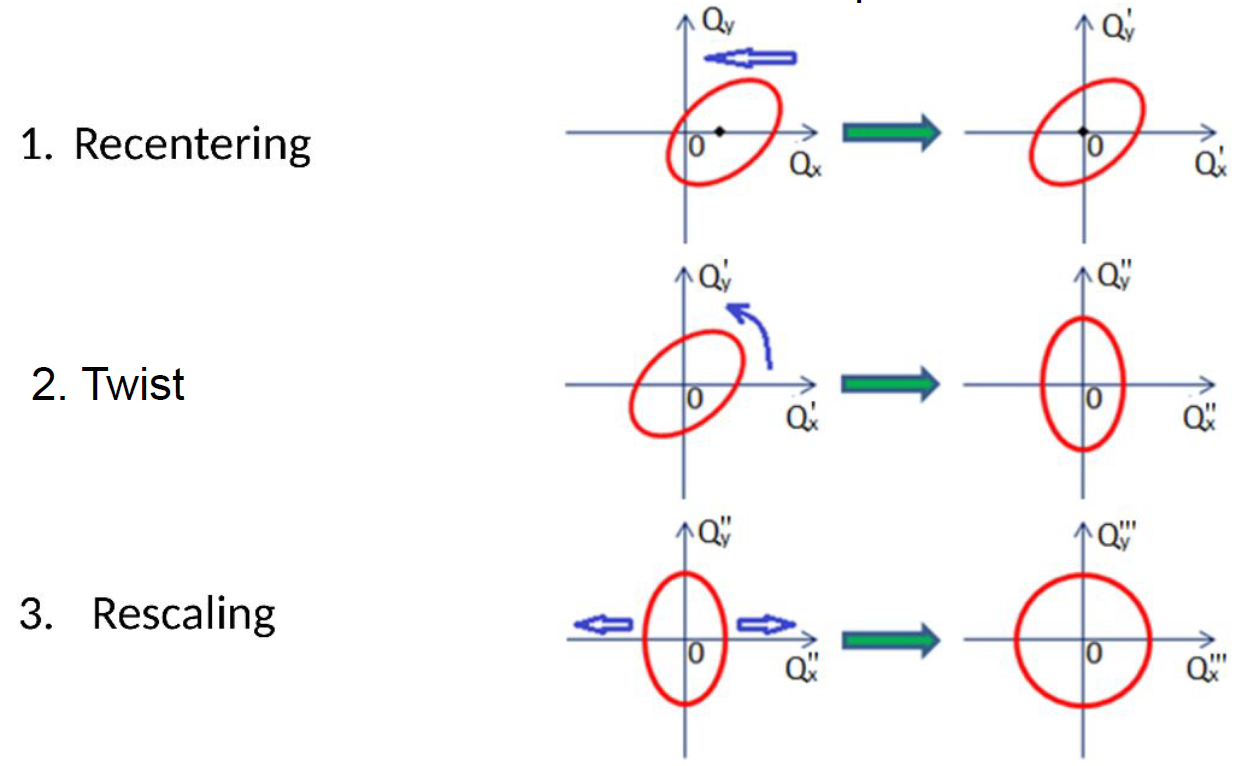
\includegraphics[width=0.5\linewidth]{images/corrections_for_nonuniformity.png}
    \caption{Схематическое представление эффекта применения каждого этапа коррекций, описанных в~\cite{Selyuzhenkov:2007zi}.}
    \label{fig:qn_corrections}
\end{figure}
Ранее описанные выше методы коррекции применялись лишь на коллайдерных экспериментах с относительно однородным аксептансом. 
Впервые коррекции рецентровки, поворота и ремасштабирования будут применятся автором для коррекции сильно неоднородного аксептанса установок HADES и BM@N.
Систематический вклад остаточной азимутальной неоднородности аксептанса детектора предлагается оцененить путём сравнением результатов полученных с использованием различных компонент $u_1$ и $Q_1$-векторов~\cite{Mamaev:2020qom,Mamaev:2023yhz}. 

\subsection{Вычисление $Q_1$ при помощи модульных детекторов}

В данной работе для восстановления плоскости симметрии используются фрагменты ядра, которые взаимодействовали с областью перекрытия лишь упруго (спектаторы). 
Спектаторные фрагменты отталкиваются областью перекрытия в плоскости реакции (см.~\ref{fig:pp_sp_rp}), поэтому могут быть использованы для реконструкции плоскости симметрии. 
Часто в экспериментах по столкновению тяжёлых ионов регистрация спектаторных частиц выполняется при помощи передних детекторов, имеющих модульную структуру. 
В таком случае $Q_n$-вектор будет определяться суммарной азимутальной анизотропией распределения сигнала по модулям:
%
\begin{equation}
    \vec{Q}_n  = \frac{1}{C} \sum_{k=1}^M w_k ( \cos n \varphi, \sin n \varphi ),
    \label{eq:module_qn}
\end{equation}
%
где $k$ --- индекс модуля, $M$ --- число модулей, использованных в построении $Q_n$-вектора, $w_k$ --- сигнал в данном модуле, $\varphi$ --- азимутальный угол данного модуля. 
Нормировочный коэффициент $C$ может также принимать значения $C=|Q_1|$ (метод плоскости события) или $C=\sum_{k=1}^M w_k$ (метод скалярного произведения).
Взвешивание на сигнал в данном модуле необходимо, поскольку в один и тот же модуль могут попасть более одной частицы.
Корреляции между $Q_n$-векторами, определёнными из разных групп модулей одного детектора также могут быть подвержены непотоковым корреляциям.
К примеру, между соседними модулями может происходить перетекание сигнала вследствие конструкционных особенностей детектора (например, в адронных калориметрах присутствует поперечное распространение ливней).
Также при распаде осколков сталкивающихся ядер, фрагменты могут вызвать отклик соседних модулей, что снова приведёт к корреляциям между модулями, которые не относятся к коллективному движению частиц.
Такие корреляции могут искажать значения разрешения $R_n$, полученного лишь при помощи $Q_n$-векторов из передних детекторов.
Автором предлагается дополнительно определить $Q_n$-вектора из треков рожденных частиц.
Это позволит внести значительное разделение между $Q_n$-векторами из передних детекторов и треков частиц.
Комбинируя различные группы $Q_n$-векторов, возможно оценить вклад непотоковых корреляций в значения $R_n$ для плоскостей симметрии спектаторов~\cite{Mamaev:2023fpr,Mamaev:2023yhz,Mamaev:2024}.

\section{Выводы к главе 1}

В главе был приведён обзор существующей литературы по коллективной анизотропии рожденных в столкновении частиц. 
Были описаны основные механизмы образования коллективной анизотропии и представлены обоснования необходимости ее измерения.
В главе изложены основные методы измерения коллективной анизотропии рожденных в столкновении частиц.
Определены единичный вектор частиц $u_n$ и вектор плоскости симметрии события $Q_n$.
Приведены экспериментальные методы оценки плоскости реакции и измерения коэффициентов коллективного потока $v_n$ в терминах $u_n$ и $Q_n$ векторов.
В главе обсуждаются преимущества и недостатки методов плоскости события и скалярного произведения для оценки коллективных потоков. 
Автором предлагается оценить систематическую ошибку измерения коэффциентов $v_n$ методом плоскости события, полученных коллаборацией HADES, путём сравнения со значениями, полученными методом скалярного произведения.
Описаны методы вычисления поправочного коэффициента разрешения, такие как метод случайных подсобытий и метод трёх подсобытий.
В главе обсуждается вклад непотоковых корреляций в вычисленные значеняи $R_n$ для методов случайного подсобытия и метода трёх подсобытий.
Автор диссертации предлагает сравнивать разрешение $R_n$, полученное с использованием различных комбинаций $Q_n$-векторов для оценки и минимизации вклада непотоковых корреляций в коэффициент разрешения. 
Сравнивая $v_n$, полученный относительно различных плоскостей симметрии $Q_n$ предлагается оценить систематическую ошибку для измеренных значений коллективных потоков. 
В главе обсуждается влияние неоднородности азимутального аксептанса детектора на измерения $v_n$.
Автором предлагается использовать коррекции, ранее опробованные на относительно однородном аксептансе коллайдерных установок, для устранения эффектов сильно неоднородного аксептанса экспериментов с фиксированной мишенью. 
Автор диссертации излагает особенности оценки плоскости реакции при помощи спектаторных передних детекторов, имеющих модульную структуру.
Приводится описание эффектов, влиящих на корреляцию между $Q_n$-векторами из модульных детекторов. 
Автором предлагается метод учёта этих эффектов при вычислении коэффициента разрешения $R_n$.           % Глава 1
\chapter{Экспериментальные установки HADES и BM@N} \label{chapt2}


\section{Ускорительный комплекс SIS-18}

Ускорительный комплекс SIS-18 состоит из линейного ускорителя UNILAC и синхротрона тяжелых ионов SIS-18.
Линейный ускоритель UNILAC способен разгонять ионы в широком диапазоне массовых чисел: от протонов до ядер урана.
Ускоритель оборудован инжектором ионов VARIS (Vacuum Arc Ion Source), способного достигать силы тока ионов до 6~мА.
При помощи вакуумно-дугового разряда тяжелые ионы испаряются с поверхности источника, а затем разделяются с помощью масс-спектрометра в подсистеме LEBT (Low Energy Beam Transport system).
Затем ионы тяжелых ядер с энергией 2.2$A$~кэВ транспортируются в инжектор High Current Injector, в котором они разгоняются до энергий 1.4$A$~МэВ и полностью лишаются электронной оболочки с помощью сверхзвукового потка газа.
В дальнейшем полностью ионизированные тяжелые ядра при энергии 11.4$A$~МэВ подаются на вход синхротнона SIS-18.

Максимальная магнитная жесткость синхротрона достигает 18~Тлм, что позволяет разогнать ядра Au$^{69+}$ до 1.25$A$~ГэВ, Ag$^{47+}$ до 1.5$A$~ГэВ и протоны до 4.5$A$~ГэВ.
Длина синхротронного кольца составляет 217~м.
Кольцо разделено на 12 идентичных секций.
Каждая секция состоит из двух дипольных магнитов для отклонения пучка, трех квадрупольных магнитов и одного секступольного магнита для фокусировки пучка.
После синхротрона ускоренные тяжелые ядра подаются на вход эксперимента HADES.

\section{Эксперимент HADES}

HADES (High Acceptance DiElectron Spectrometer) является многофункциональной экспериментальной установкой с фиксированной мишенью.
Установка базируется на отдельном выводе ускорителя SIS-18 в центре по изучению тяжелых ионов имени Гельмгольца ГСИ, в городе Дармштадт.
Физическая программа установки состоит из экспериментов по столкновению как адронов так и тяжелых ядер и направлена на изучение механизмов образования странных частиц и роли барионных резонансов в этих процессах. 
Схема экспериментальной установки приведена на рис.~\ref{fig:hades_bmn_layouts}~\cite{HADES:2009aat}.
Эксперимент состоит из 6 секторов, которые расположены радиально симметрично относительно оси пучка.
Далле представлено описание основных детекторных подсистем.
%
\begin{figure}[ht]
\begin{center}
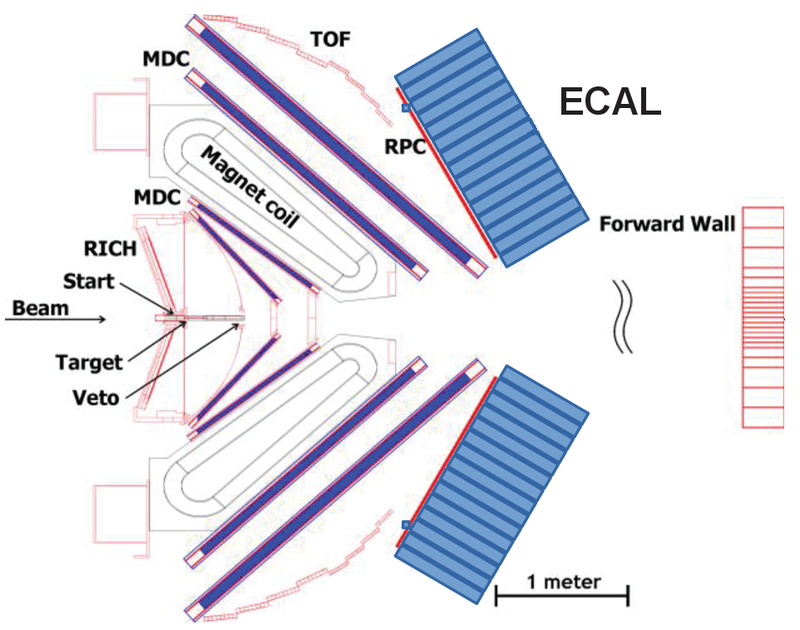
\includegraphics[width=0.75\linewidth]{images/hades_layout.jpg}
\caption{Схема эксперимента HADES}
\label{fig:hades_bmn_layouts}
\end{center}
\end{figure}

\subsection{ Мишень }

Мишень, на которой происходит взаимодействия ускоренных ядер представляет из себя 15 каптоновых полосок, закрепленных на углеволоконной трубке.
На каптоновые полоски толщиной 7~мкм наклеены диски из золота (серебра) толщиной 25~мкм.
Расстояние между полосками составляет 4 мм. 
Общая толщина мишени --- 375~мкм, что соответствует общей вероятности взаимодействия в 1.5\%.
Фотография мишени приведена на рис.~\ref{fig:hades_target}. 
%
\begin{figure}[ht]
\begin{center}
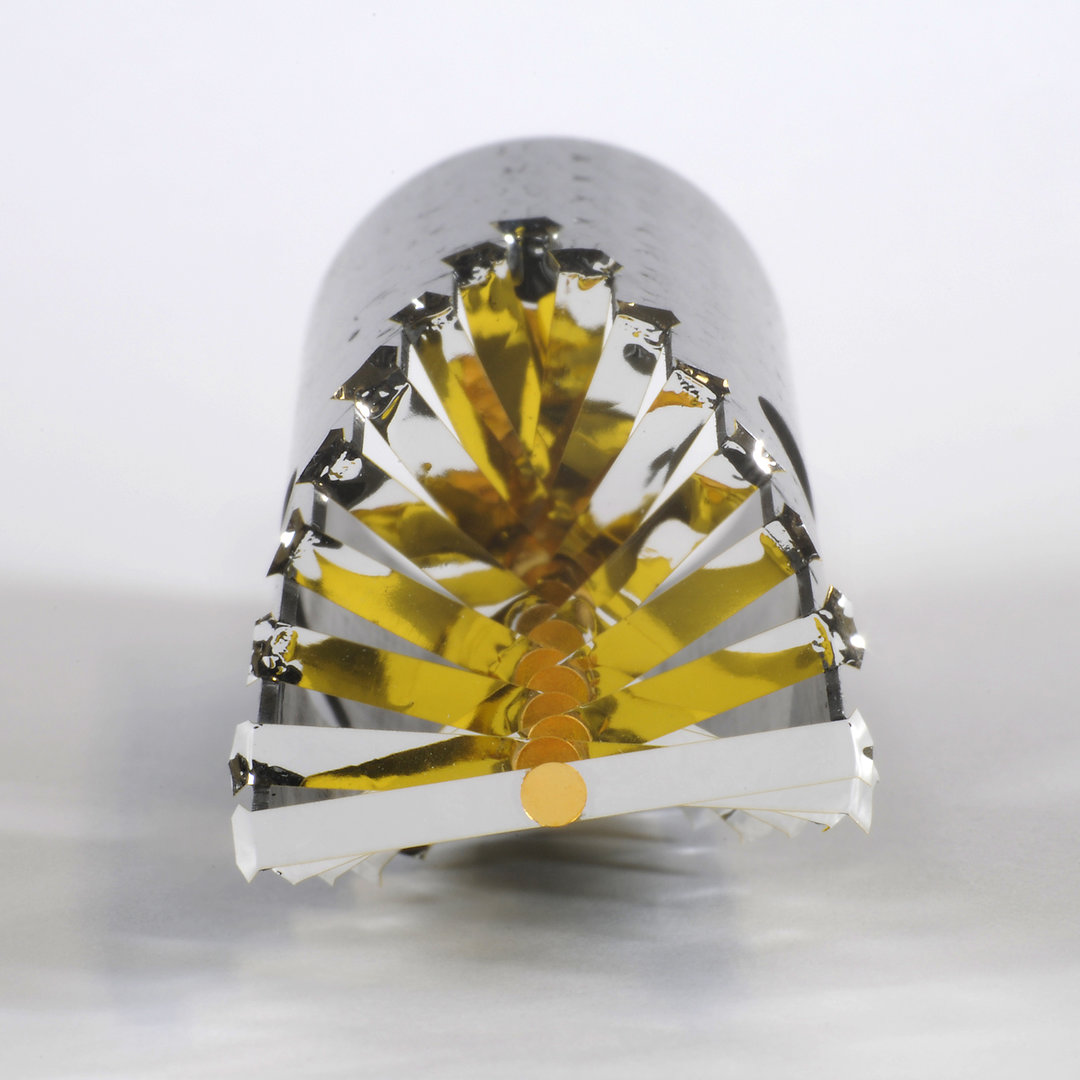
\includegraphics[width=0.55\linewidth]{images/hades_target.jpg}
\caption{ Фотография мишени для сеанса Au~+~Au при энергии 1.23$A$~ГэВ.  }
\label{fig:hades_target}
\end{center}
\end{figure}

\subsection{ Магнитный спектрометр }

Магнитный спектрометр состоит из 6 тороидальных сверхпроводящих магнитов и 24 многопроволочных дрейфовых камер (MDC).
В каждом из 6 секторов две плоскости MDC располагаются до магнита и 2 --- после. 
Реконструкция импульса производится посредством итеративного решения уравнения движения частиц в локальном магнитном поле при помощи метода Рунге-Кутта.
Заряд частицы определяется по отклонению частицы в магнитном поле: положительно заряженные частиц отклоняются, уменьшая значения полярного угла $\theta$, отрицательно заряженные --- увеличивают значения полярного угла.
Реконструкция импульса может выполняться для большого окна полярных углов в широком диапазоне $p$: от 0.1 до 2 ГэВ/c.
Магнитное поле позволяет измерять импульсы заряженных частиц с разрешением для электронов с энергией 0.15~МэВ $\Delta p/p \approx$ 2\% и протонов с энергией около 1~ГэВ $\Delta p/p \approx$ 4\%.  

\subsection{ Магнит }

Магнитное поле создаётся при помощи сверхпроводящего магнита ISLE, который состоит из 6 секторов, которые в первом приближении отклоняют заряженные частицы, изменяя лишь их полярный угол $\theta$.
При максимальной силе тока $I$=3500~А, максимум магнитного поля в 3 Тл достигается на краях магнита, а в центре сектора составляет 0.9 Тл.
Магнит фокусирует положительно заряженные частиц в направлении оси Z.
Сверхпроводящие катушки состоят из ниобий-титанового сплава, инкапсулированного в медную матрицу.
Медная матрица необходима для механической стабильности конструкции.
Вся сборка упакована в катушки, окруженные аллюминиевым корпусом, который предотвращает механические повреждения в случае внезапного отключения магнитного поля.
Катушки окружены системой охлаждения работающей на жидком азоте при температуре 85~К.
Токопроводящие эллементы дополнительно охлаждаются однофазным гелием при температуре 4.7~К и давлении 2.8 бар.

\subsection{ Камеры MDC }

Площадь чувсвительного материала внутренних камер составляет 0.35 м$^2$, а внешних --- 3.21 м$^2$.
Наименьшая чувствительная единица называется чувствительной ячейкой и представляет из себя плоскость с одной чувствительной и двумя потенциальными проволоками.
Катод и анод сделаны из отожженного алюминия, а чувствительная проволока --- из покрытого золотом вольфрама.
Каждая секция состоит из порядка 1100 чувствительных ячеек, организованных в 6 слоёв, каждый из которых повёрнут на 20 градусов друг относительно друга ($\pm0^{\circ}$, $\pm20^{\circ}$, $\pm40^{\circ}$).
Такая организация чувствительного объема позволяет достичь равномерного разрешения по азимутальному (85-125 мкм) и полярному (35-50 мкм) углам.
Первый слой MDC заполнен смесью газов Ar+CO$_{2}$ в пропорциях 70:30.
Оставшиеся три слоя работают на смеси аргона и изобутана. 
Заряженная частица, пролетая через чувствительную зону детектора ионизирует газ, и высвобожденные электроны дрейфуют в сторону чувствительной проволоки.
Собранный заряд детектируется и восстанавливается пространственная координата в которой произошла ионизация газа.

\subsection{START и VETO детекторы}

START и VETO детекторы предназначены для детектирования событий столкновения ядер.
START и VETO используются для регистрации времени столкновения $T_0$ и выработки триггеров.
Совместно с времяпролётными детекторами TOF и RPC, START и VETO позволяют измерять время пролёта заряженных частиц.
Детектор VETO был разработан для подавления эффекта pile-up, когда на мишени происходит более одного взаимодействия.
Детектор имеет малую толщину, приблизительно 60 мкм, и состоит из алмазов, покрытых тонкой плёнкой металла. 
START детектор в свою очередь собран из алмазов с металлическим напылением, нанесенных тонким слоем на полоски из хромированного золота.
Всего 16 полосок шириной 200 мкм с интервалом в 90 мкм обеспечивают высокую точность регистрации налетающего ядра по $x$ и $y$.

\subsection{Времяпролётный детекторы TOF и RPC}

Времяпролётный детектор TOF состоит из 384 сцинтилярных стержней из поливинилтолуола, который обладает малой длиной ослабления света, высоким сцинтиляционным выходом и коротким временем распада.
Поперечные размеры внутренних стержней составляют $20 \times 20$ мм$^2$ и внешних --- $30\times30$ мм$^2$.
Проходя через сцинтиляционный стержень, заряженная частица возбуждает атомы чувствительного материала, которые затем возвращаются в основное состояние через эмиссию света.
Излученный свет распространяется в оба конца детектора, где считывается при помощи двух фотоумножителей.
По разности времён регистрации света на двух концах сцинтиляционного стержня затем рассчитывается $x$-координата попадания частицы.
Также по амплитуде сигнала рассчитываются энергопотери заряженной частицы при прохождении через материал детектора.

Для увеличения аксептанса времяпролетной системы, ближе к оси пучка за детекторами TOF находятся 6 резистивных плоскостных детекторов (RPC). 
Каждая секция состоит из двух частично перекрывающихся слоёв, в каждом из которых находится 31 стрип RPC.
Каждый RPC собран из чередующихся слоев аллюминиевых электродов и изолятора --- стекла --- в газовом объеме, заполненном смесью $SF_6$ и $C_2H_2F_4$.
Заряженные частицы ионизируют газ и дельта-электроны ускоряются магнитным полем в сторону анода, создавая электронную лавину.

\subsection{ Трекинговая система }

Трекинговая система HADES, предназначенная для реконструкции траекторий заряженных частиц, состоит из четырёх плоскостей многопроволочных дрейфовых камер (MDC).
Для измерения импульса заряженных частиц, между второй и третьей плоскостями, располагается сверхпроводящий магнит, отклоняющий проходящие через него частицы.
На рис.~\ref{fig:hades_tracking} схематически изображена трекинговая система эксперимента HADES.
Треки заряженных частиц совмещаются из траекторий в плоскостях I и II, и III и IV методом Рунге-Кутта.
Импульс заряженной частицы восстанавливается по отклонению в магнтином поле между плоскостями II и III 
%
\begin{figure}[ht]
\begin{center}
    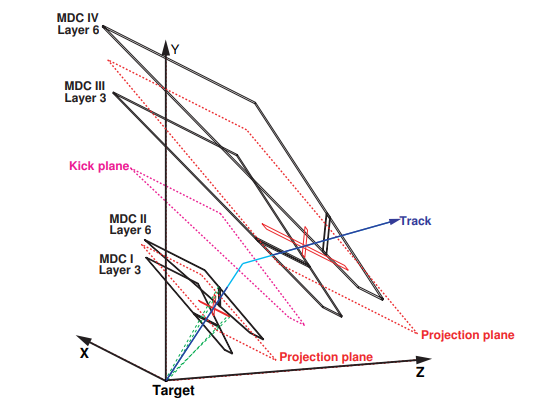
\includegraphics[width=0.55\linewidth]{images/hades_tracking_system.png}
    \caption{Схмеатическое изображение трекинговой системы эксперимента HADES.}
    \label{fig:hades_tracking}
\end{center}
\end{figure}

\subsection{Передний годоскоп Forward Wall}

Для регистрации фрагментов сталкивающихся ядер, взаимодействовавших с областью перекрытия лишь упруго (спектаторы), спектрометр HADES оборудован годоскопом FW.
Детектор имеет модульную структуру и способен измерять заряд фрагментов-спектаторов.
Размер модулей годоскопа увеличивается от центральных к периферическим и составляет $40\times40$, $80\times80$ и $160\times160$~мм$^2$ соответственно.
Схематично, расположение модулей в годоскопе представлено на рис.~\ref{fig:hodo_layout}.
%
\begin{figure}[ht]
\begin{center}
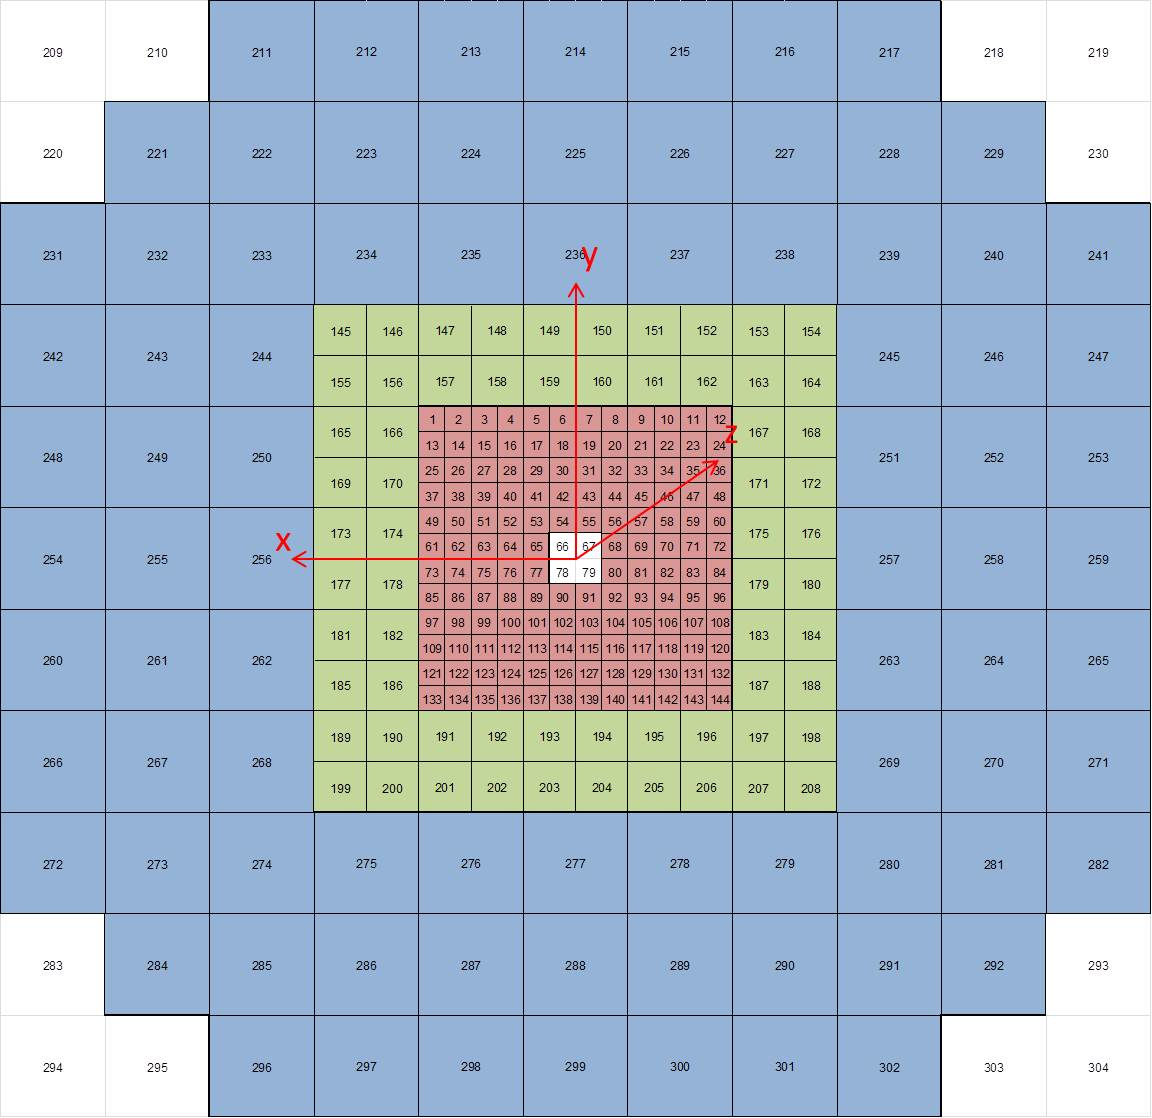
\includegraphics[width=0.55\linewidth]{images/FW_layout.jpg}
\caption{Схема расположения модулей переднего годоскопа FW.}
\label{fig:hodo_layout}
\end{center}
\end{figure}

\section{Описание экспериментальной установки BM@N}

\subsection{Ускорительный комплекс NUCLOTRON-NICA}

Эксперимент BM@N располагается на выведенном пучке ускорителя NUCLOTRON, который является частью ускорительного комплеса NICA, ОИЯИ, Дубна.
Линейный ускоритель тяжелых ионов Linac инжектирует пучок в кольцевой ускоритель Boster.
После ускорения тяжелых ионов в кольце Booster до энергии в $0.5A$~ГэВ, пучок подаётся на NUCLOTRON.
Максимальные энергии, достижимые Nuclotron составляют до $4.5A$~ГэВ.
После ускорения ядер до необходимой энергии, пучок может быть отправлен как на эксперимент BM@N, так и на коллайдер NICA.

\subsection{Схема установки}

BM@N является экспериментом с фиксированной мишенью.
Схема экспериментальной установке представлена на рис.~\ref{fig:bmn_layout}.
%
\begin{figure}[ht]
\begin{center}
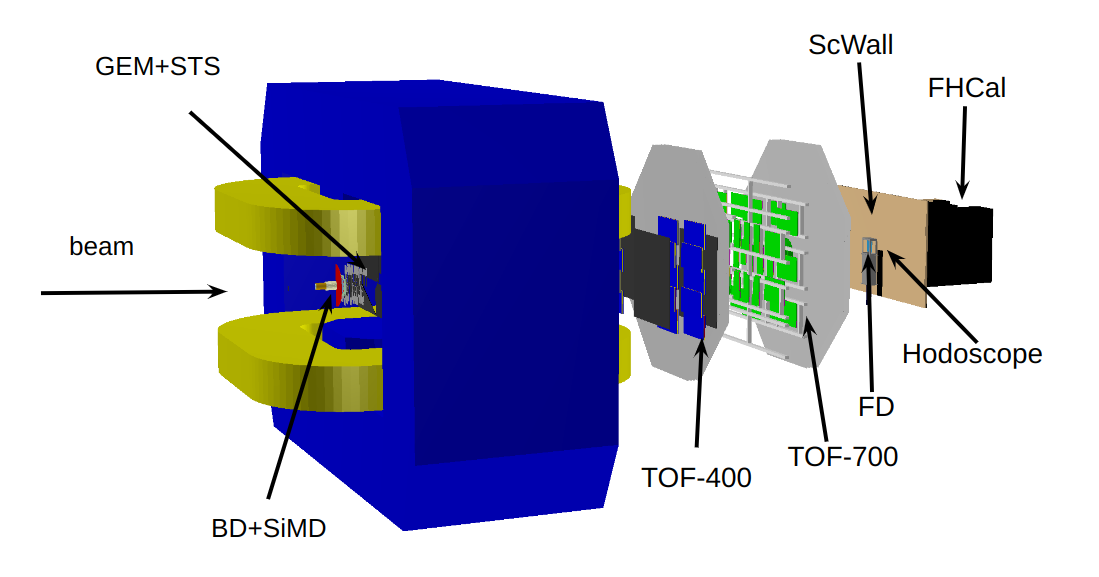
\includegraphics[width=0.95\linewidth]{images/BM@N_layout.png}
\caption{Схема эксперимента BM@N.}
\label{fig:bmn_layout}
\end{center}
\end{figure}

\subsection{Трекинговая система}

Система реконструкции траекторий заряженных частиц в эксперименте BM@N состоит из четырех станций кремниевых детекторов (Silicon) и семи станций газо-электронных умножителей (GEM). 
В отличие от HADES, трекинговая система целиком находится в магнитном поле дипольного магнита что позволяет с большой точностью восстанавливать импульсы рожденных в столкновении заряженных частиц.
На рис.~\ref{fig:bmn_tracking} представлено схематическое изображение трекинговой системы в эксперименте BM@N.
Траектории заряженных частиц отклоняются магнитным полем дипольного магнита, что позволяет восстанавливать импульс заряженных частиц.
Вакуумная пучковая труба позволяет минимизировать столкновения ядер цезия с атомами азота, кислорода и прочими примесями.
Поскольку вакуумная труба также расположена в магнитном поле, она имеет искривлённую форму для свободного прохождения невзаимодействоваших ядер пучка.  
%
\begin{figure}[ht]
\begin{center}
    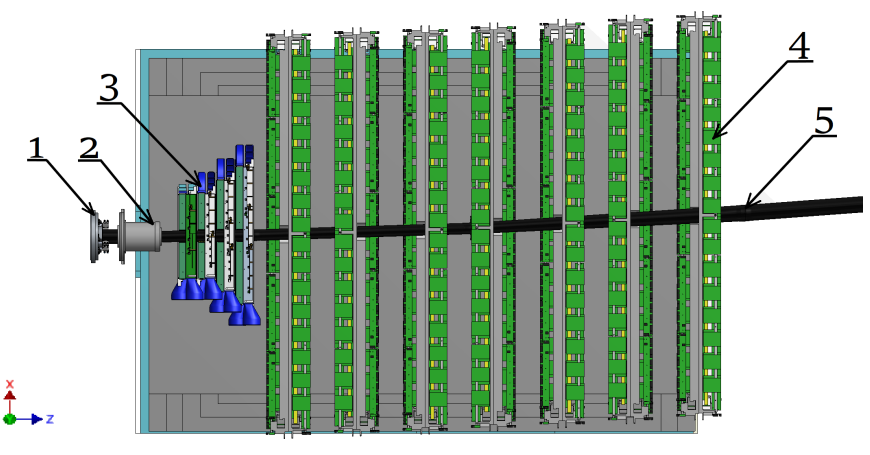
\includegraphics[width=0.75\linewidth]{images/bmn_tracking_system.png}
    \caption{Схематическое изображение трекинговой системы в эксперименте BM@N. Цифрами (1) обозначена мишень,
    (2) --- Barell Detector, (3) --- STS, (4) --- GEM, (5) --- Beam Pipe }
    \label{fig:bmn_tracking}
\end{center}
\end{figure}


\subsection{Времяпролётные детекторы TOF-400 и TOF-700}

В эксперименте BM@N идентификация заряженных частиц может выполняться только времяпролётным методом, используя информацию с двух станций времяпролётных детекторов, расположенных на расстоянии 400 и 700~см от мишении (TOF-400 и TOF-700 соответственно).
Подсистема TOF-400 состоит из двух половин, размещенных симметрично относительно оси пучка.
Каждая половина собрана из 5 MRPC детекторов.
Каждый детектор покрывает площадь $60\times30$~см$^2$.
Полный геометрический аксептанс всей сборки равен $1.1\times1.3$~м$^2$.
Дектор TOF-700 покрывает площадь в $3.2\time2.2$~м$^2$.
Подсистема также собрана из MRPC детекторов.

На рис.~\ref{fig:bmn_beta_pq} показано распределение заряженных частиц по относительной скорости $\beta=v/c$ и импульсу деленному на заряд $p/q$.
%
\begin{figure}[ht]
\begin{center}
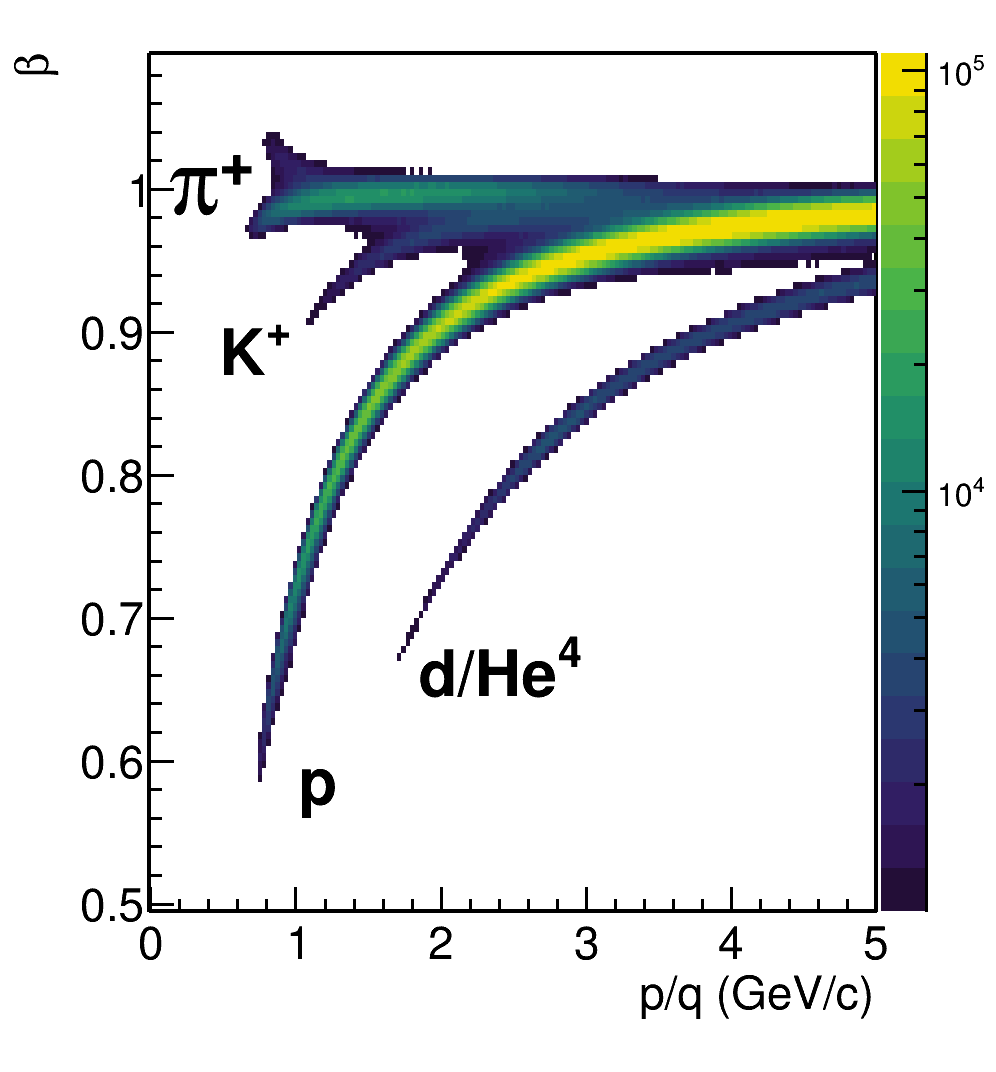
\includegraphics[width=0.55\linewidth]{images/beta_pq.png}
\caption{Распределение заряженных частиц по относительной скорости $\beta=v/c$ и импульсу деленному на заряд $p/q$.}
\label{fig:bmn_beta_pq}
\end{center}
\end{figure}

\subsection{Передний адронный калориметр FHCal}

В эксперименте BM@N энерговыделение спектаторных фрагментов измеряется при помощи переднего адронного калориметра FHCal.
Адронный калориметр состоит из 54 модулей, их размеры --- $15\times15$ и $20\times20$~см.
Схема расположения модулей калориметра представлена на рис.~\ref{fig:fhcal_layout} справа.
Большие модули ($20\times20$~см) обозначены желтым цветом, малые модули ($15\times15$) обозначены синим цветом. 
%
\begin{figure}[ht]
\begin{center}
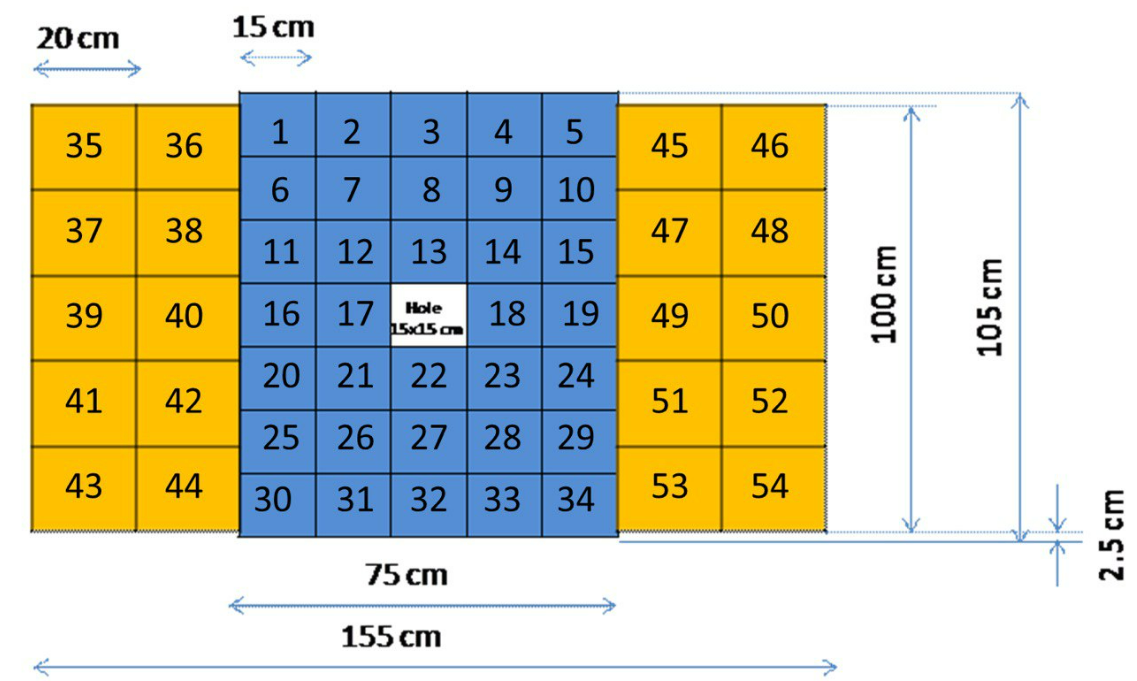
\includegraphics[width=0.55\linewidth]{images/FHCal_modules.png}
\caption{Схема расположения модулей переднего адронного калориметра FHCal.}
\label{fig:fhcal_layout}
\end{center}
\end{figure}

\section{Выводы к главе 2}

В главе описывается устройство экспериментальной установки HADES. 
Рассмотрены принципы работы основных детекторных подсистем, таких как трекинговая система, триггерная система, времяпролётная система и передний годоскоп Forward Wall.
В главе приведено краткое описание установки BM@N и ее детекторов.
Рассмотрены принципы работы трекинговой системы, описано устройство времяпролётной системы и переднего адронного калориметра FHCal.
           % Глава 2
\chapter{Экспериментальные методы измерения коллективной анизотропии}

\section{Эксперимент HADES}

\subsection{Критерии отбора столкновений и рожденных частиц}

В работе приводятся результаты анализа экспериментальных данных, полученные из столкновений ядер Au+Au при энергии $E_{kin}=$1.23$A$~ГэВ а также ядер Ag+Ag при энергиях $E_{kin}=$1.23$A$ и 1.58$A$~ГэВ, полученные на установке HADES.
Всего было проанализировано около 100 миллионов столкновений Au+Au и по 500 миллионов столкновений для Ag+Ag при обеих энергиях.
Для исследования использовались столкновения разделенные по времени и восстановленной вершиной лежащей в области мишени.
Траектории заряженных частиц были отобраны на основании качества аппроксимации трека.
Для отбора первичных частиц использовался критерий на минимальное расстояние между ее траекторией и первичной вершиной. 

Для анализа использовались события столкновений тяжелых ядер, вершина которых лежала в следующих границах: $\sqrt{x_v^2+y_v^2}<3$~мм и $z_v \in (-60, 0)$~мм.
Для измерения направленного потока использовались траектории заряженных частиц которые были экстраполированы в вершину столкновения.
Траектории которые имели расстояние до восстановленной точки взаимодействия более 10~мм не использовались в анализе.

\subsection{Определение центральности столкновения}

Центральность столкновений в эксперименте HADES была определена на основе количества срабатываний времяпролетной системы.
Метод Монте-Карло Глаубера был использован для восстановления распределения геометрических параметров столкновения, таких как средний прицельный параметр, числа нуклонов-спектаторов и числа нуклонов-партисипантов (для деталей см.~\cite{HADES:2017def}).
На рис.~\ref{fig:hades_multiplicity} представлено Распределение множественности срабатываний времяпролетной системы в столкновениях Au + Au при энергии $E_{kin}$=1.23$A$~ГэВ и Ag + Ag при $E_{kin}$=1.23$A$~ГэВ и $E_{kin}$=1.58$A$~ГэВ.
Наибольшая множественность наблюдается в столкновениях Au + Au, поскольку число нуклов в ядрах золота почти в 2 раза больше.
\begin{figure}[ht]
\begin{center}
    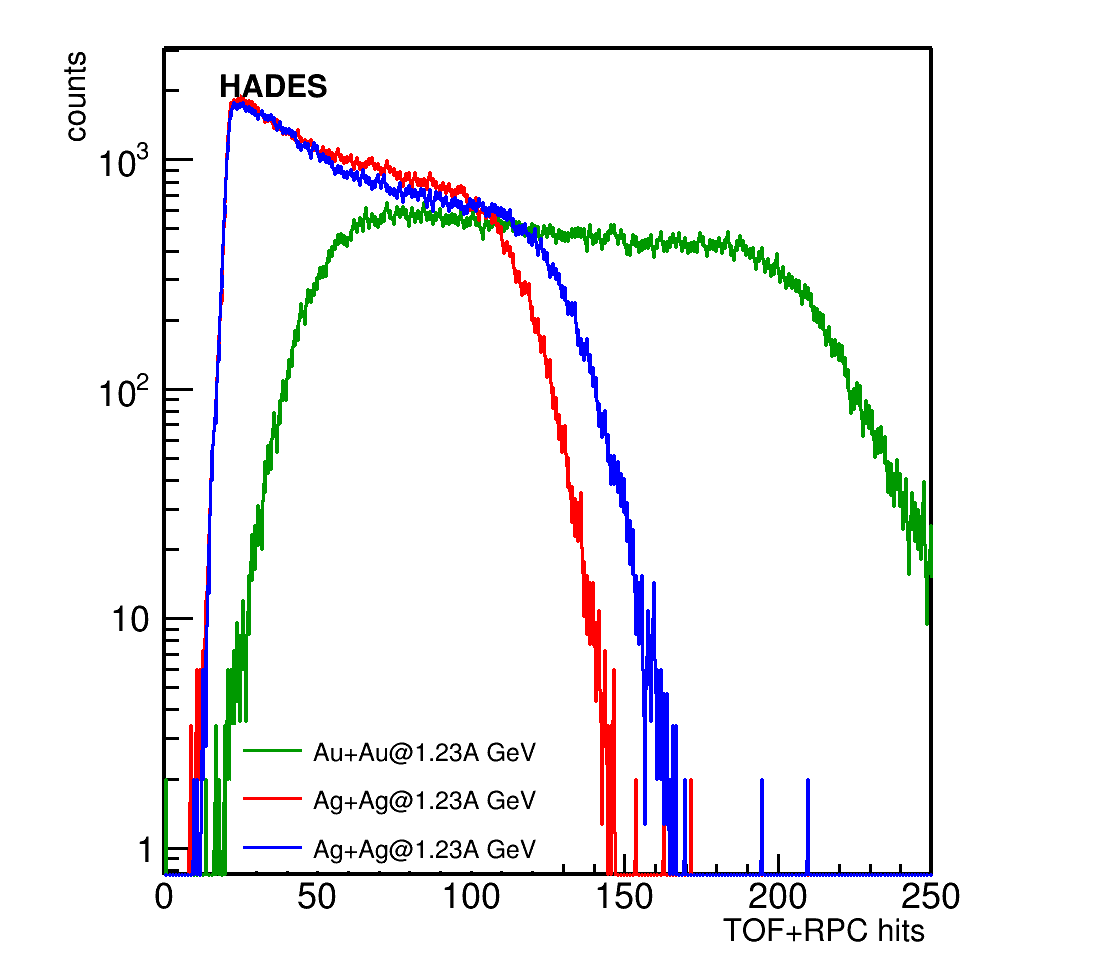
\includegraphics[width=0.55\linewidth]{images/multiplicity.png}
    \caption{Распределение множественности заряженных срабатываний времяпролетной системы в столкновениях Au + Au при энергии $E_{kin}$=1.23$A$~ГэВ и Ag + Ag при $E_{kin}$=1.23$A$~ГэВ и $E_{kin}$=1.58$A$~ГэВ.
    }
    \label{fig:hades_multiplicity}
\end{center}
\end{figure}

Для каждой из анализируемых систем методом Монте-Карло Глаубера была измерена центральность столкновения. 
На рис.~\ref{fig:hades_centrality} представлено Распределение множественности срабатываний во времяпролётной системе в столкновениях Ag + Ag при энергии $E_{kin}$=1.58$A$~ГэВ. Вертикальными линиями обозначены границы классов центральности.
Аппроксимация множественности методом Монте-Карло Глаубера довольно хорошо описывает экспериментальное распределение в классе центральности 0-30\%.
Дальнейшее расхождение объясняется эффективностью центрального триггера.
Регистрация столкновения в эксперименте происходит по величине, пропорциональной множественности рожденных частиц.
Поэтому события с маленькой множественностью могут быть отброшены системой отбора событий столкновения.
Таким образом, экспериментальное распределение множественности частиц, рожденных в столкновении систематически смещено в область более высоких множественностей.
Монте-Карло розыгрыш множественности при помощи метода Глаубера и отрицательного биномиального распределения помогают оценить это смещение и восстановить реальное распрделение множественности.  
%
\begin{figure}[ht]
\begin{center}
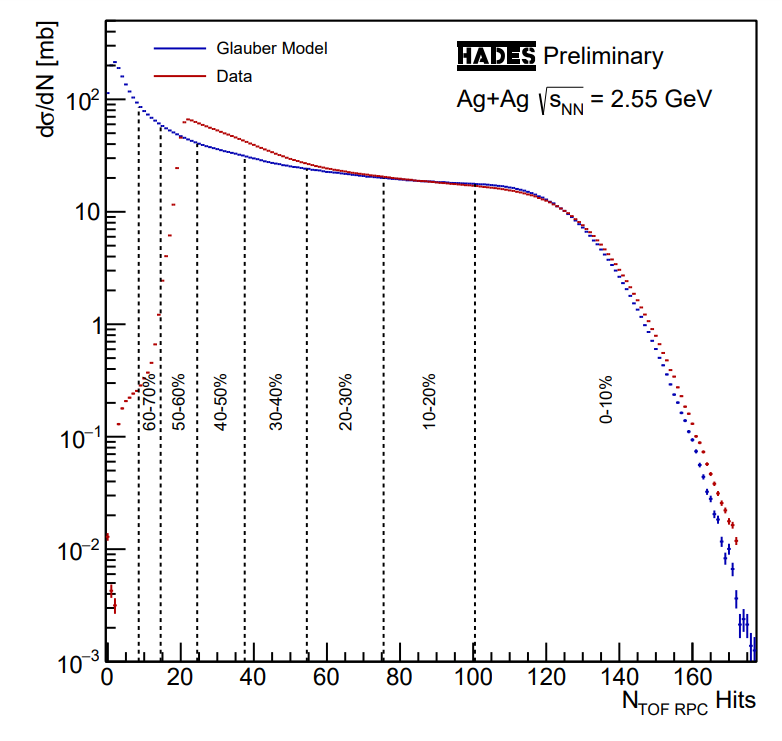
\includegraphics[width=0.55\linewidth]{images/hades_mult.png}
\caption{Распределение множественности заряженных срабатываний времяпролетной системы в столкновениях Ag + Ag при энергии $E_{kin}$=1.58$A$~ГэВ. Вертикальными линиями обозначены границы классов центральности.}
\label{fig:hades_centrality}
\end{center}
\end{figure}


\subsection{Эффективность реконструкции протонов}

Эффективность реконструкции протонов была рассчитана при помощи Монте-Карло моделирования отклика детектора. 
В качестве входных данных использовалась физическая модель DCM-QGSM-SMM~\cite{Botvina:1994vj, Baznat:2019iom}.
Реалистичный отклик детекторов был смоделирован при помощи программного пакета GEANT3. 
Далее по модели отклика детектора была произведена реалистичная реконструкция.
Эффективность реконструкции определяется формулой:
\begin{equation}
    e(y, p_T) = \frac{ N_{rec}(y,p_T) }{ N_{sim}(y, p_T) },
\end{equation}
где $e(y, p_T)$ --- эффективность реконструкции для данных значений поперечного импульса ($p_T$) и быстроты ($y$), $N_{rec}$ --- число реконструированных частиц, $N_{sim}$ --- число смоделированных частиц.
На рис.~\ref{fig:hades_efficiency} представлена эффективность реконструкции протонов как функция быстроты ($y$) и поперечного импульса ($p_T$) для столкновений Au + Au при энергии $E_{kin}$=1.23$A$~ГэВ (слева), Ag + Ag при энергии $E_{kin}$=1.23$A$~ГэВ (посередине) и $E_{kin}$=1.58$A$~ГэВ (справа).
%
\begin{figure}[ht]
\begin{center}
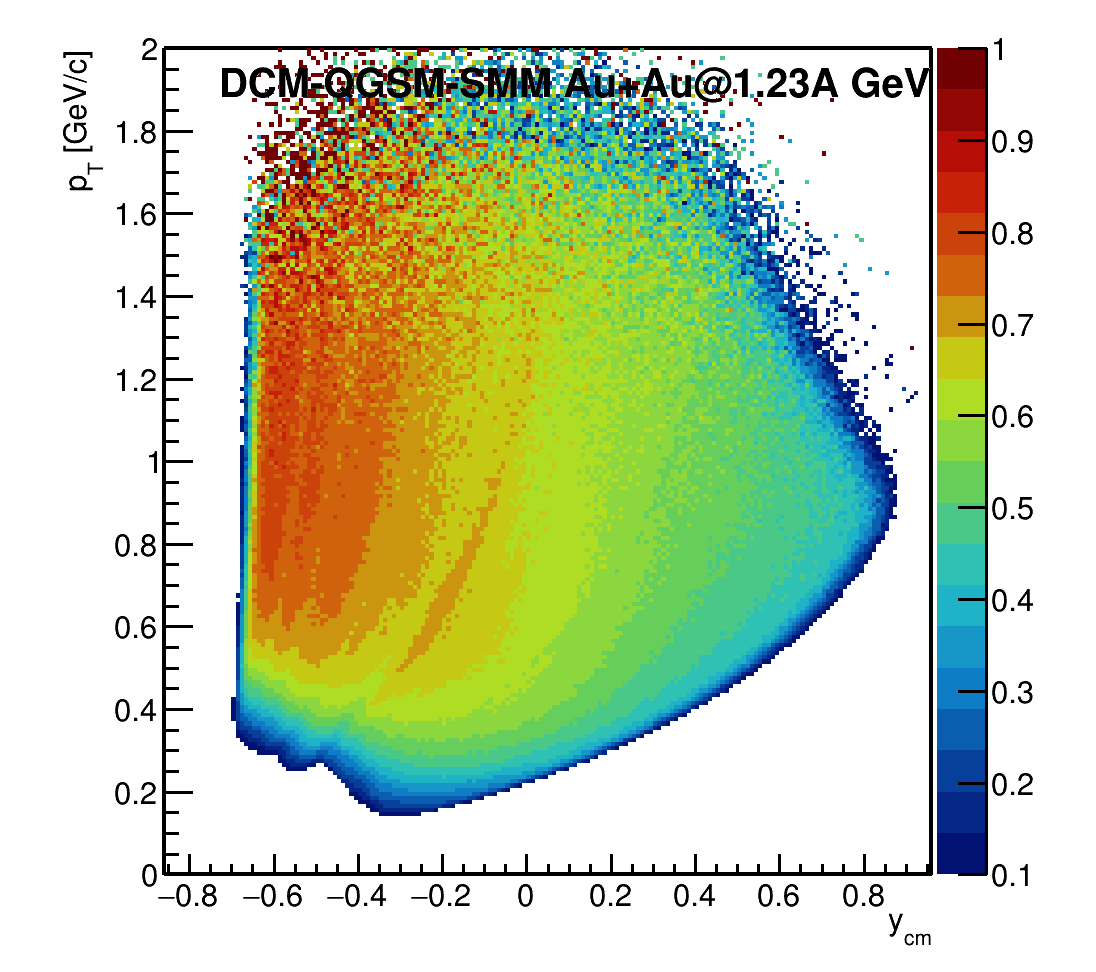
\includegraphics[width=0.3\linewidth]{images/au123_efficiency_y_pT.png}
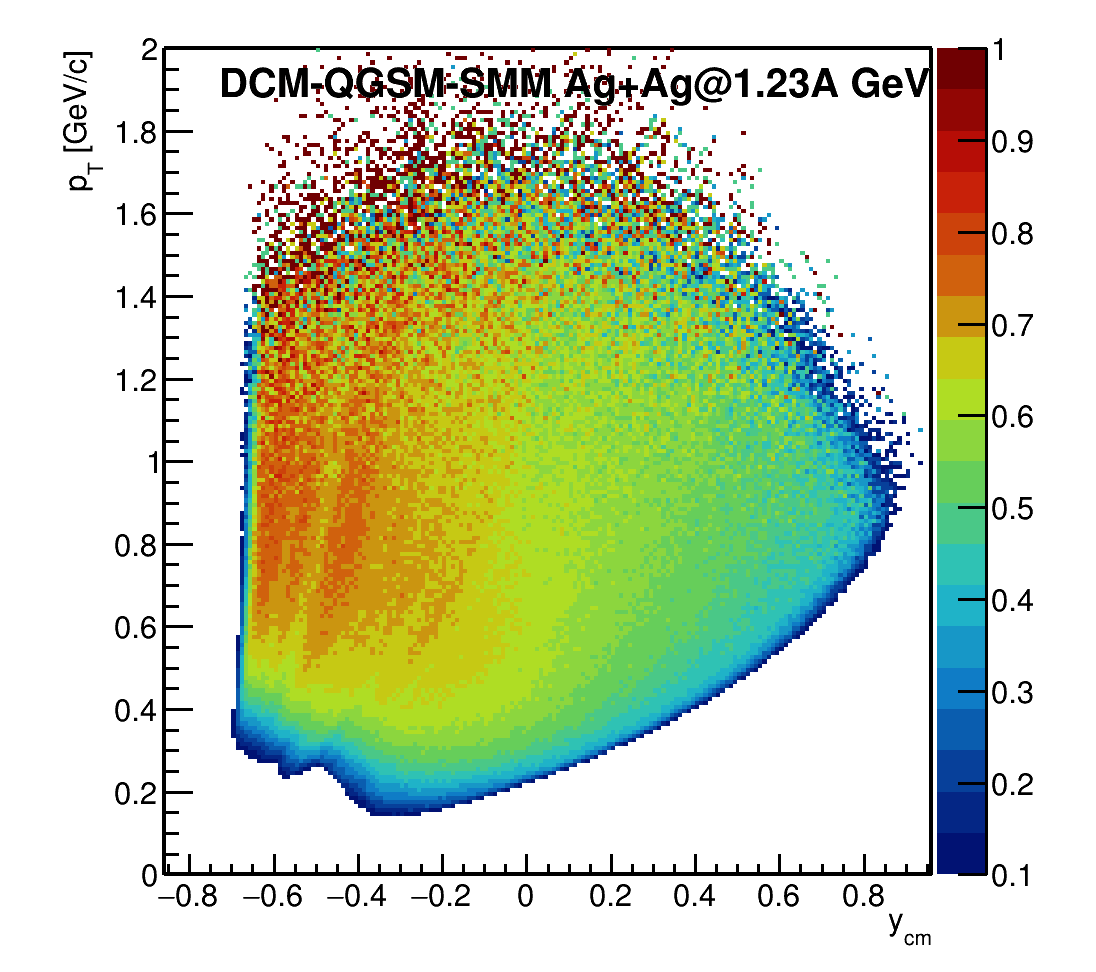
\includegraphics[width=0.3\linewidth]{images/ag123_efficiency_y_pT.png}
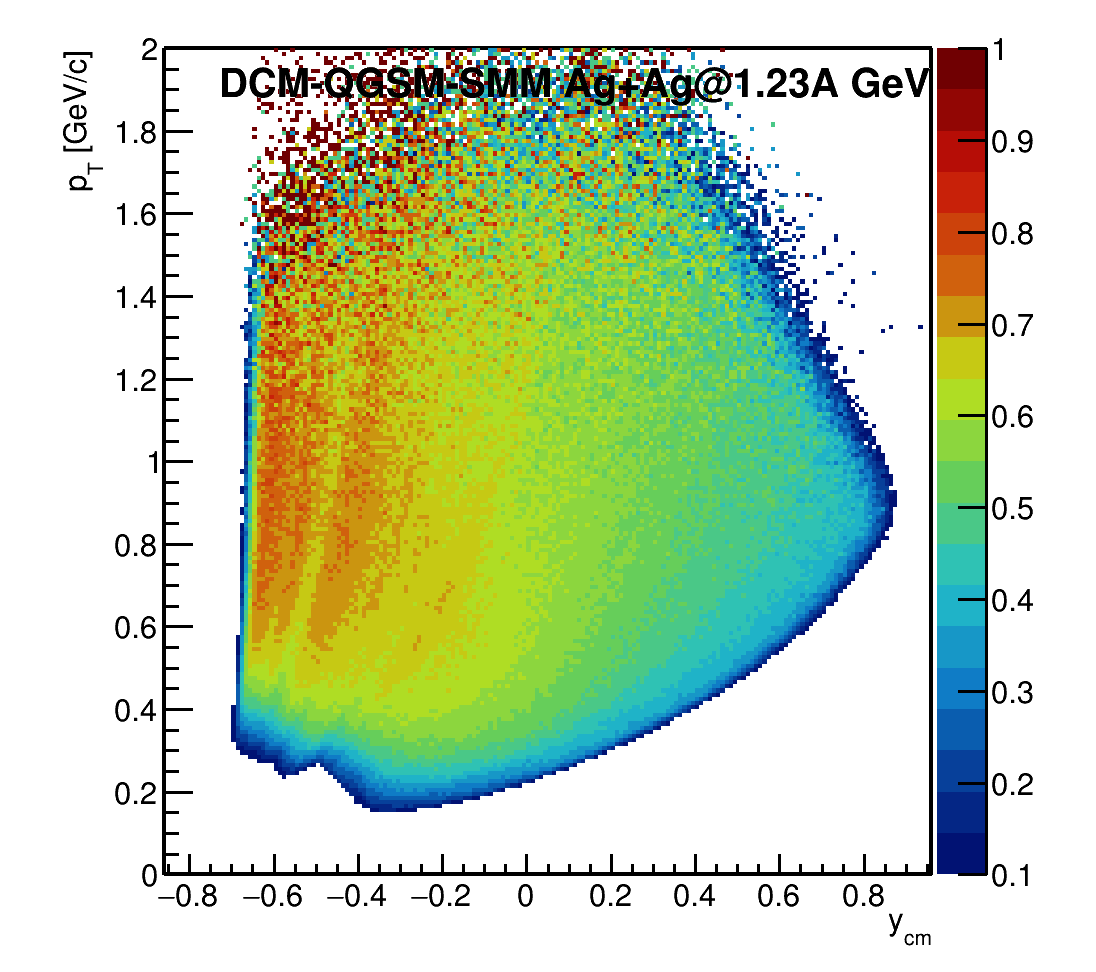
\includegraphics[width=0.3\linewidth]{images/ag158_efficiency_y_pT.png}
\caption{Эффективность реконструкции протонов как функция быстроты ($y$) и поперечного импульса ($p_T$) для столкновений Au + Au при энергии $E_{kin}$=1.23$A$~ГэВ (слева), Ag + Ag при энергии $E_{kin}$=1.23$A$~ГэВ (посередине) и $E_{kin}$=1.58$A$~ГэВ (справа). }
\label{fig:hades_efficiency}
\end{center}
\end{figure}

\subsection{Идентификация протонов времяпролётным методом}

Для измерения времени пролёта, установка HADES оборудована времяпролётными системами TOF и RPC, которые располагаются за трекинговой системой (см. рис.~\ref{fig:hades_bmn_layouts}).
Детектор TOF состоит из сцинтиляционных стержней, ориентированных радиально.
Детекторная подсистема RPC представляет из себя набор резистивных камер.
Идентификация частиц проводилась одновременно времяпролётным методом и по энерговыделению в камерах MDC.
На рис.~\ref{fig:hades_pid} представлено распределение заряженных частиц, зарегистрированных трекинговой системой HADES по относительной скорости $\beta$ и импульсу делённому на заряд $p/q$.
Используя соотношение:
\begin{equation}
    p = \frac{ m\beta }{ \sqrt{1-\beta^2} },
\end{equation}
где $p$ --- импульс частицы, $m$ --- ее масса, $\beta=v/c$, ее относительная скорость, можно рассчитать массу частицы.
%
\begin{figure}[ht]
    \begin{center}
    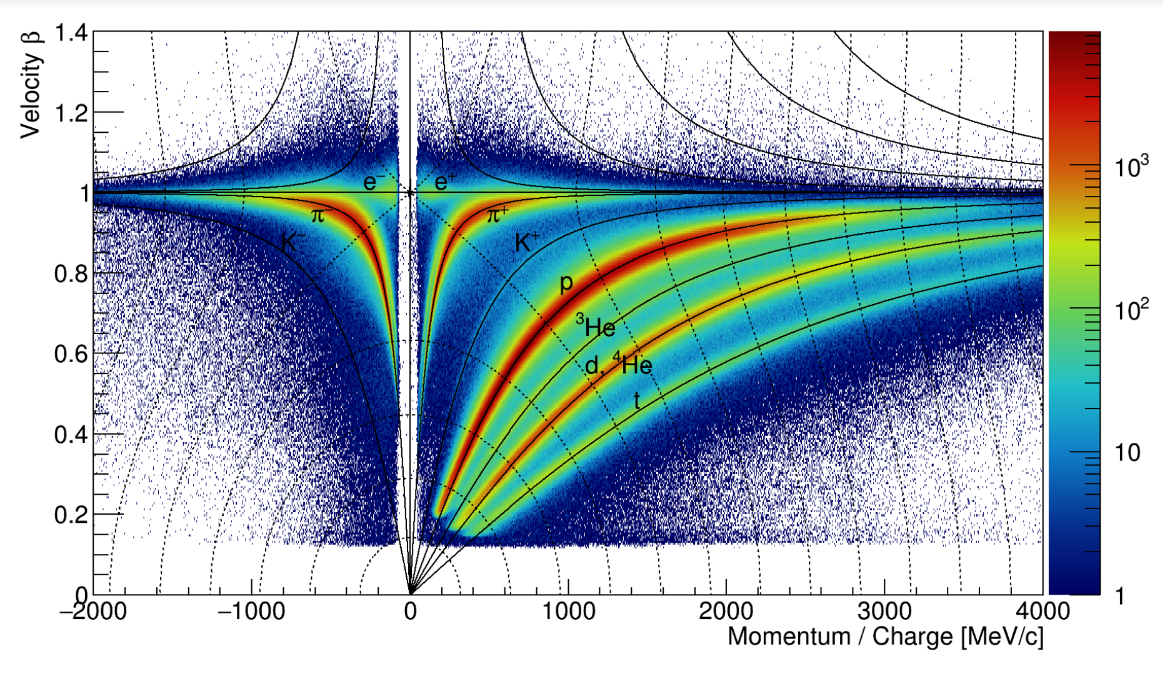
\includegraphics[width=0.95\linewidth]{images/hades_pid_plot.png}
    \caption{Распределение заряженных частиц, зарегистрированных трекинговой системой HADES по относительной скорости $\beta$ и импульсу делённому на заряд $p/q$.}
    \label{fig:hades_pid}
    \end{center}
    \end{figure}
    
Распределение заряженных частиц, зарегистрированных трекинговой системой HADES по квадрату массы $m^2$ и импульсу делённому на заряд $p/q$ представлено на рис.~\ref{fig:hades_m2_pq} (слева).
Ожидается, что массы рожденных частиц, измеренные времяпролётным методом будут распределены согласно нормальному распределению.
Среднее этого распределения для каждого типа частиц не должно зависить от импульса частицы, однако в эксперименте наблюдается сдвиг в сторону меньших значений для протонного пика.
Этот систмематический сдвиг может быть объяснён ошибкой при измерении частиц с малыми импульсами.
Большая кривизна траектории может приводить к ошибкам при ее реконструкции.
Ширина распределения для каждого вида частиц увеличивается с ростом импульса.
Этот эффект объясняется ограниченным разрешением времяпролётной системы, в которой при больших импульсах время пролёта восстанавливается с большей относительной ошибкой.
Каждый из пиков для разных типов частиц аппроксимируется функцией гаусса в узких диапазонах импульса.
Затем на основании этих аппроксимаций происходит отбор кандидатов в частицы для каждого типа.
Отобранные протоны представлены на рис.~\ref{fig:hades_m2_pq} (справа).
%
\begin{figure}[ht]
\begin{center}
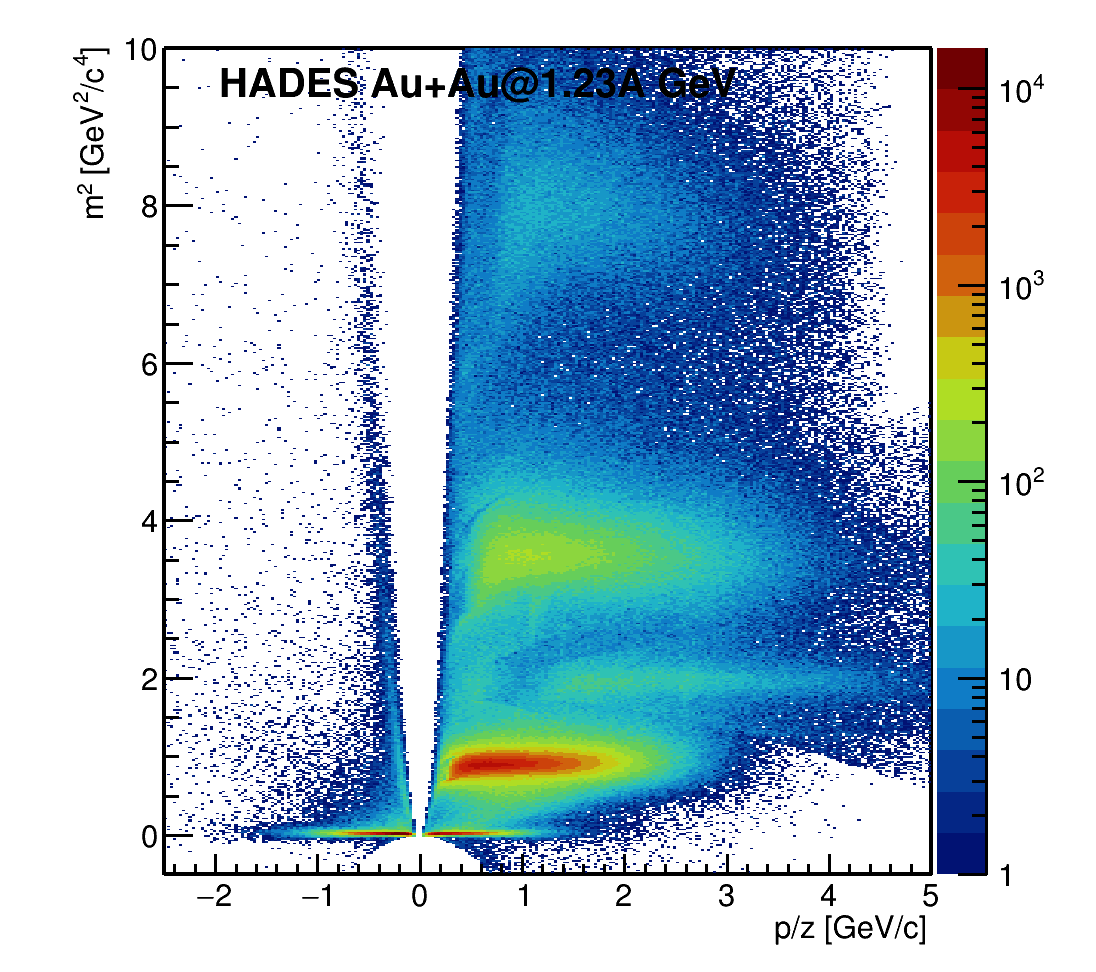
\includegraphics[width=0.45\linewidth]{images/au123_m2_vs_pq_all.png}
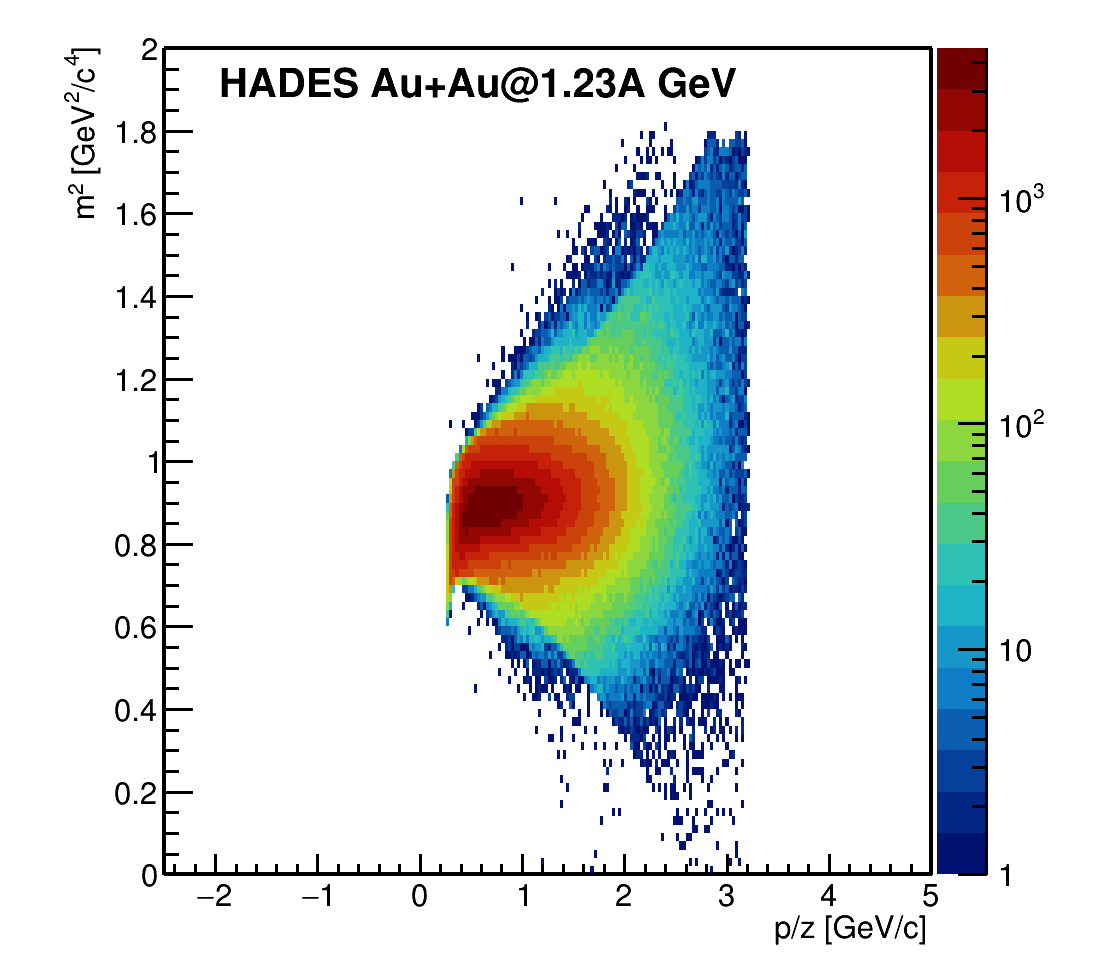
\includegraphics[width=0.45\linewidth]{images/au123_m2_vs_pq_protons.png}
\caption{Распределение заряженных частиц, зарегистрированных трекинговой системой HADES по квадрату массы деленному на квадрат заряда $m^2/q^2$ и импульсу делённому на заряд $p/q$: Для всех заряженных частиц (слева), для отобранных протонов (справа).}
\label{fig:hades_m2_pq}
\end{center}
\end{figure}

\subsection{Кинематические области используемые для определения $Q_1$ векторов}

Оценка плоскости симметрии в работе производилась по асимметрии распределения заряда спектаторов в детекторе FW. 
Для оценки систематической ошибки вызванной непотоковыми корреляциями были введены 2 дополнительных $Q_1$-вектора из треков заряженных частиц.
Векторы $Q_1$ были построены из протонов c поперечным импульсом $p_T < 2.0$~ГэВ с быстротами $0.35 < y_{cm} < 0.55$ (Mf) и $-0.55 < y_{cm} < -0.35$ (Mb).
Модули детектора FW были разделены на 3 группы: центральные (W1), средние (W2) и периферические (W3).
Схематически расположение полученных векторов в плоскости $\eta$-$p_T$ изображено на рис~\ref{fig:hades_qvectors}.
%
\begin{figure}[ht]
\begin{center}
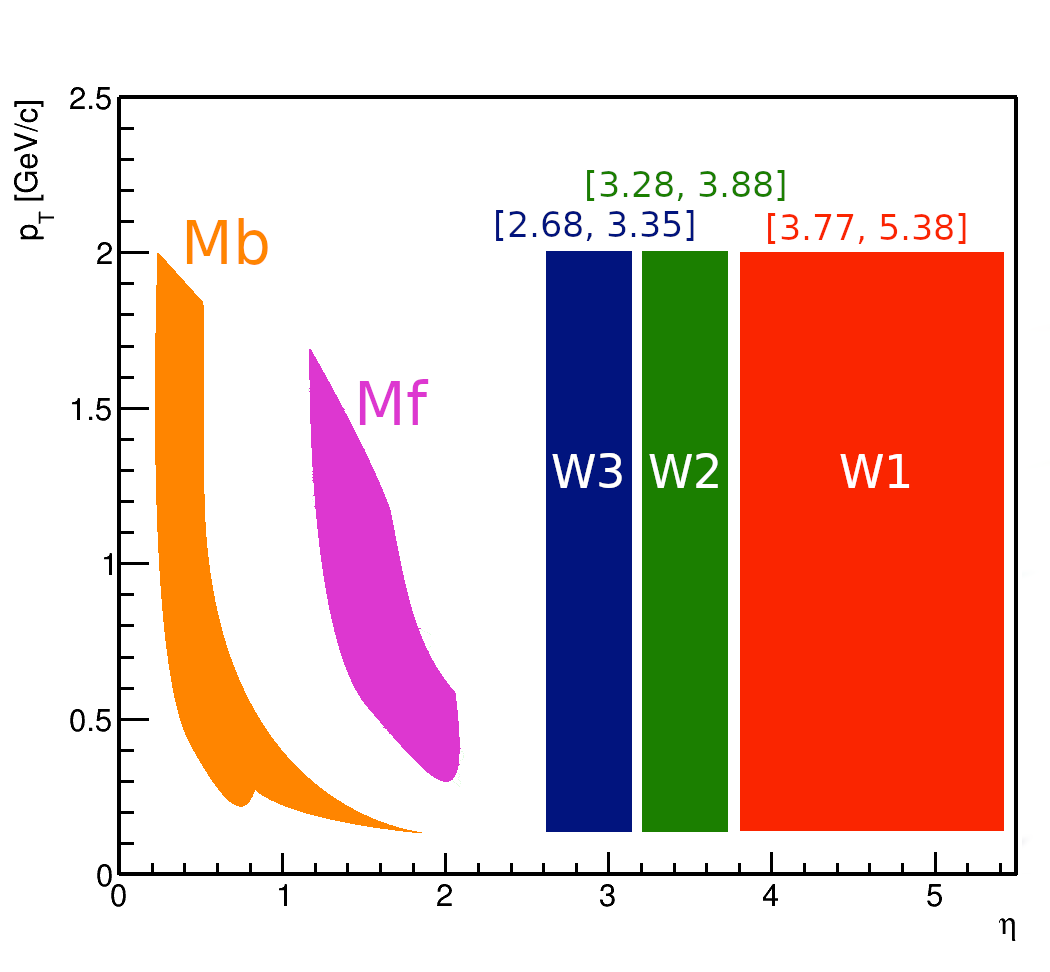
\includegraphics[width=0.75\linewidth]{images/eta_pt_qvectors.png}
\caption{Aксептанс по псевдобыстроте $\eta$ для подсобытий из FW и поперечному импульсу $p_T$ для подсобытий из MDC, использованных для расчета направленного потока протонов в столкновениях ядер золота и серебра.}
\label{fig:hades_qvectors}
\end{center}
\end{figure}
%

\subsection{Коррекция азимутальной анизотропии аксептанса детектора}

Для коррекции азимутальной неоднородноссти аксептанса был использован метод, предложенный в~\cite{Selyuzhenkov:2007zi}.
Данный метод основан на предположении, что азимутальное распределение частиц, рожденных в столкновении должно быть изотропным, поскольку угол плоскости реакции от события к событию распределен равномерно.
Азимутальная неоднородность чувствительного объема детектора вносит искажения в азимутальное распределение зарегистрированных частиц. 
Для коррекции на этот эффект, в статье~\cite{Selyuzhenkov:2007zi} вводятся поправки перецентровки, поворота и ремасштабирования. 
Схематически, действие этих поправок представлено на рис.~\ref{fig:qn_corrections}.
%
\begin{figure}[ht]
\begin{center}
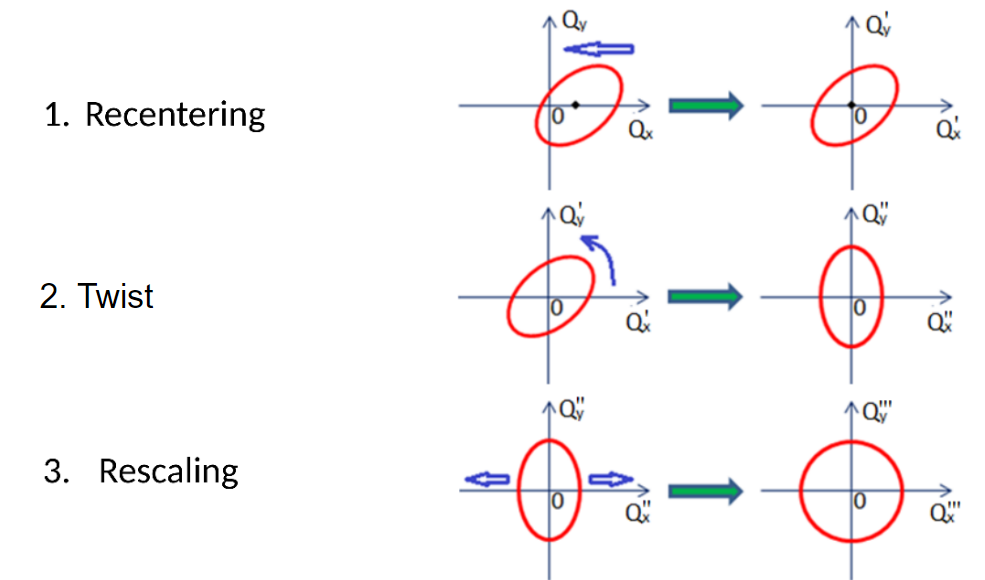
\includegraphics[width=0.75\linewidth]{images/qntools_corrections.png}
\caption{Схематическое изображение поправок предложенных в~\cite{Selyuzhenkov:2007zi}.}
\label{fig:qn_corrections}
\end{center}
\end{figure}
%

Описанные выше поправки применялись для коррекции азимутальной неоднородности аксептанса детектора мультидифференциально.
Для $Q_1$-векторов коррекции применялись в каждом классе центральности от 0\% до 40\% с шагом 5\%.
Для поправок на азимутальную неоднородность трекинга, коррекции на $u_1$-вектор применялись аналогично в каждом классе центральности а также дифференциально по поперечному импульсу $p_T$ и быстроте $y_{cm}$. 
Остаточные эффекты азимутальной неоднородности аксептанса в данной работе оцениваются как разность между корреляцией компонент $u_1$ и $Q_1$-векторов:
\begin{equation}
    \delta_{acc.} = | \langle x_1 X_1 \rangle - \langle y_1 Y_1 \rangle |,
\end{equation}
где $\delta_{acc.}$ --- остаточная ошибка после применения коррекций, $x_1$ и $y_1$, и $X_1$ и $Y_1$ --- компоненты $u_1$ и $Q_1$-векторов соответственно. 

Сравнение $v_1^{uncorr.}$, полученного с использованием различных компонент $u_1$ и $Q_1$-векторов, представлено на рис~\ref{fig:hades_uq_corr}. 
Направленный поток не корректирован на разрешение плоскости симметрии для оценки вклада неоднородного аксептанса трекинговой системы. 
После применения поправок на азимутальную анизотропию аксептанса, остаточный эффект составляет 2\%.
%
\begin{figure}[ht]
\begin{center}
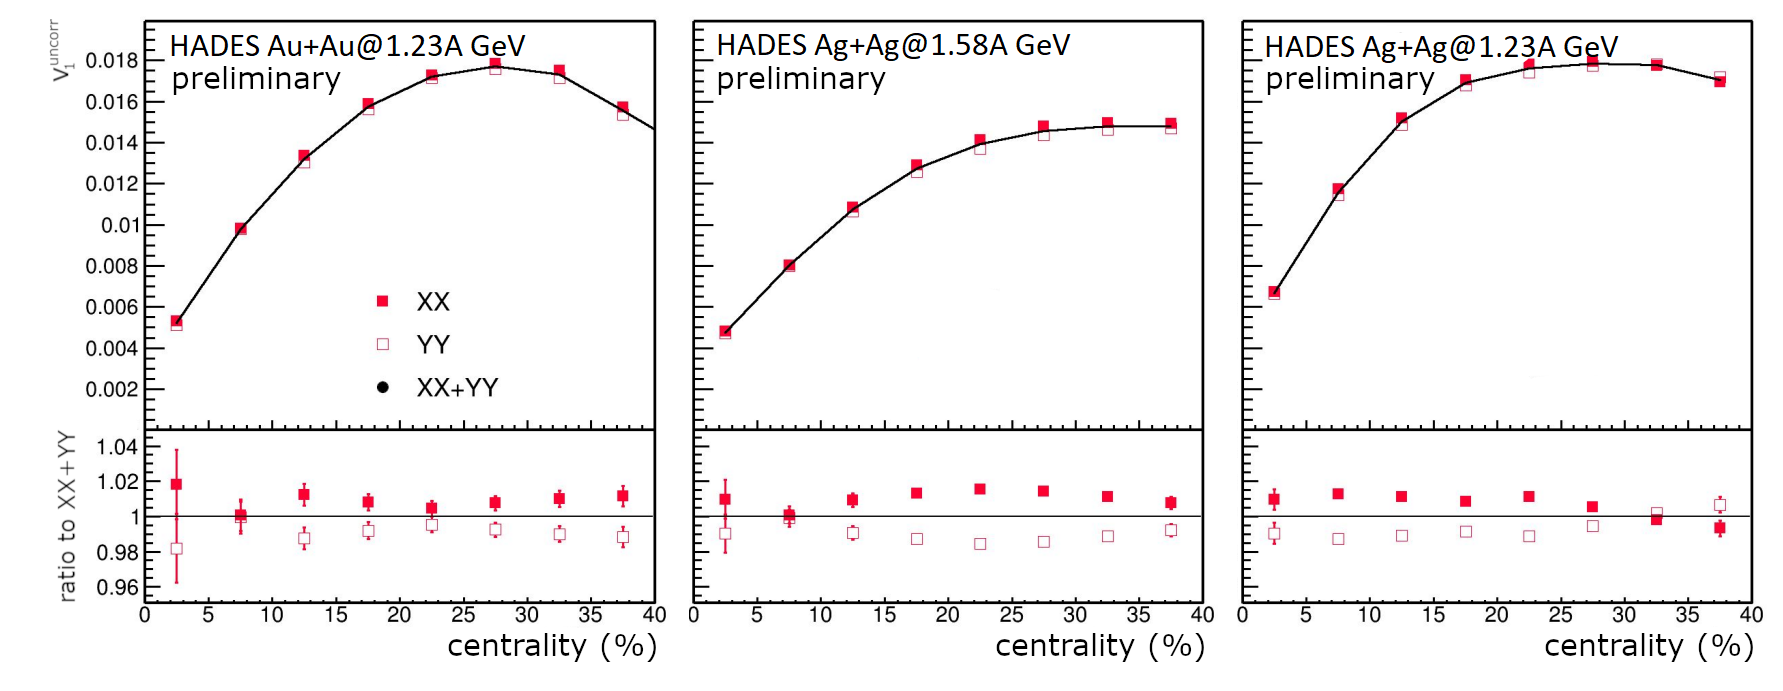
\includegraphics[width=0.75\linewidth]{images/hades_u1W1_centrality.png}
\caption{Сравнение компонент корреляции $\langle u_1 Q_1 \rangle$ после применения поправок на азимутальную неоднородность детектора для столкновений Au+Au@1.23A ГэВ (слева), Ag+Ag@1.23A ГэВ (посередине) и Ag+Ag@1.58A ГэВ (справа)}
\label{fig:hades_uq_corr}
\end{center}
\end{figure}
%

\subsection{Вычисление поравочного коэффициента разрешения $R_1$}

Для рассчета разрешения методом случайных подсобытий два вектора были определены из модулей детектора FW.
Модули были распределены в две группы случайным образом для каждого события.
На рис.~\ref{fig:hades_R1_rs} представлено разрешение плоскости симметрии рассчитанное методом случайных подсобытий как функция центральности столкновения.
Основным недостатком данного метода является отсутствие возможности сравнить полученные значения с другими оценками разрешения плоскости симметрии.
%
\begin{figure}[ht]
\begin{center}
    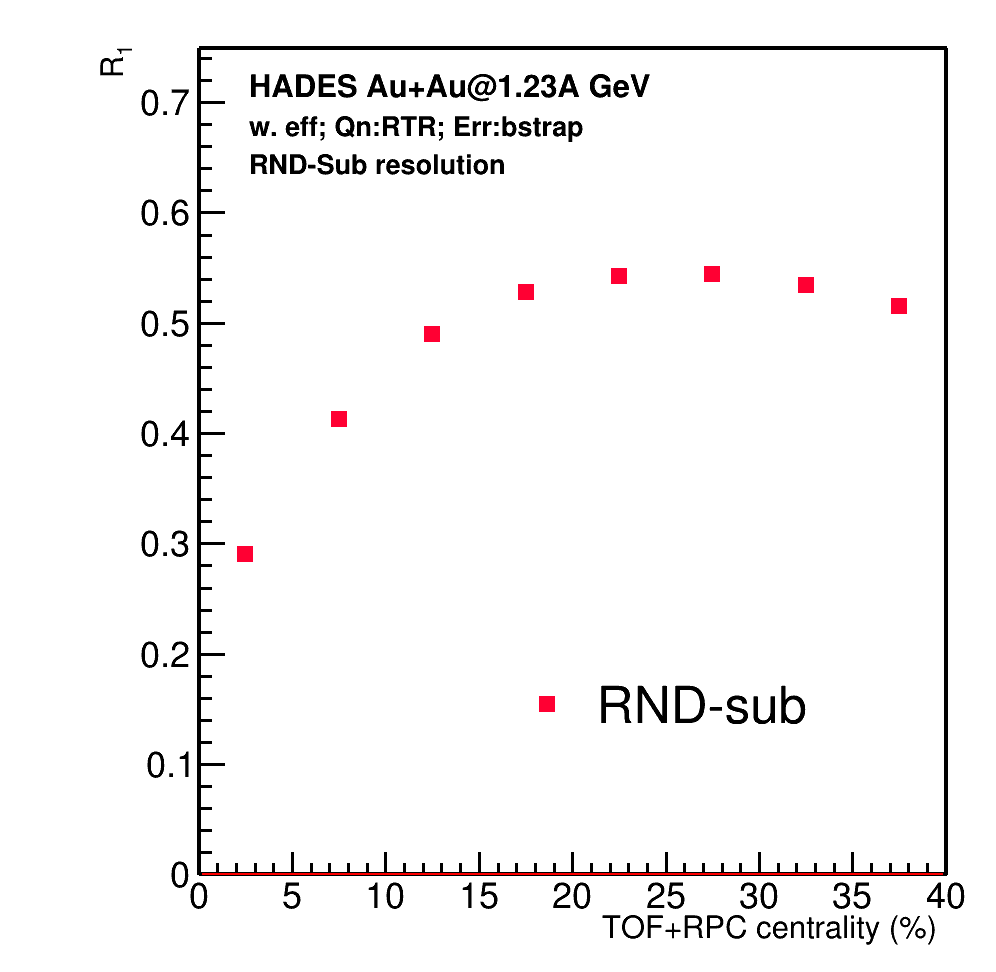
\includegraphics[width=0.3\linewidth]{images/R1_au123_rnd_centrality.png}
    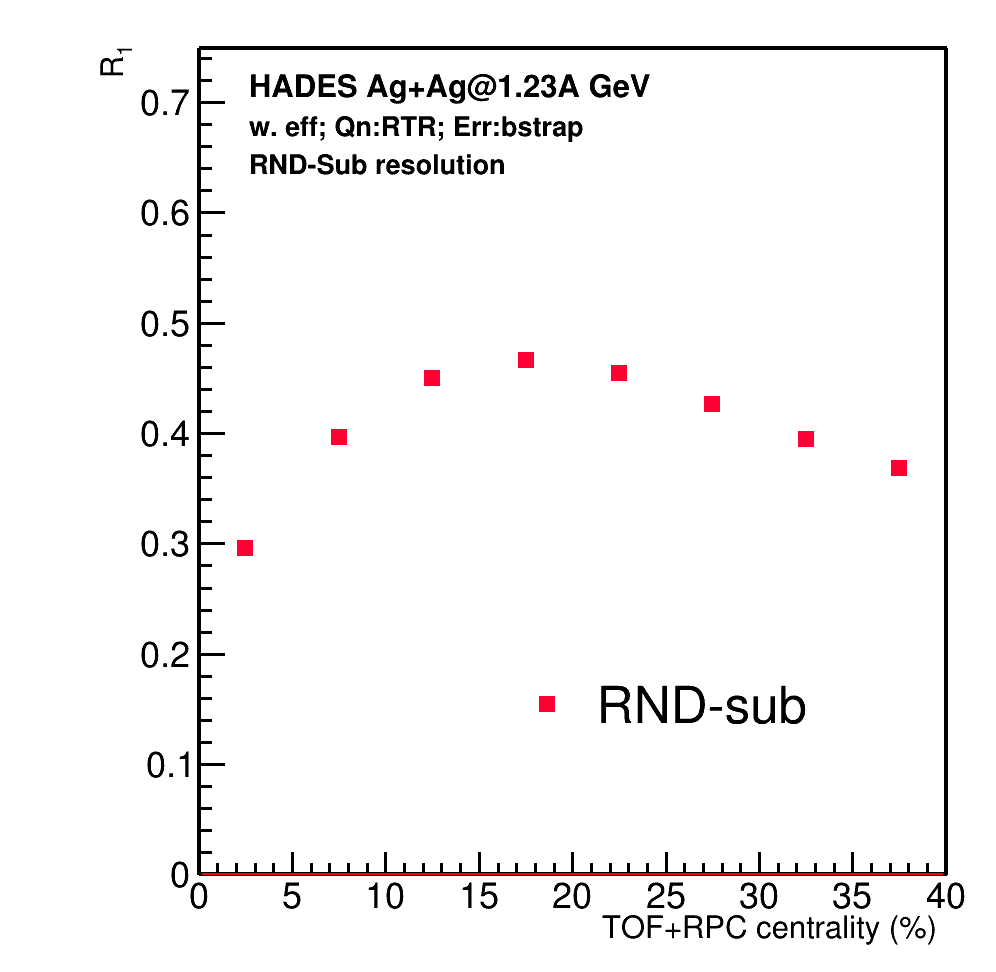
\includegraphics[width=0.3\linewidth]{images/R1_ag123_rnd_centrality.png}
    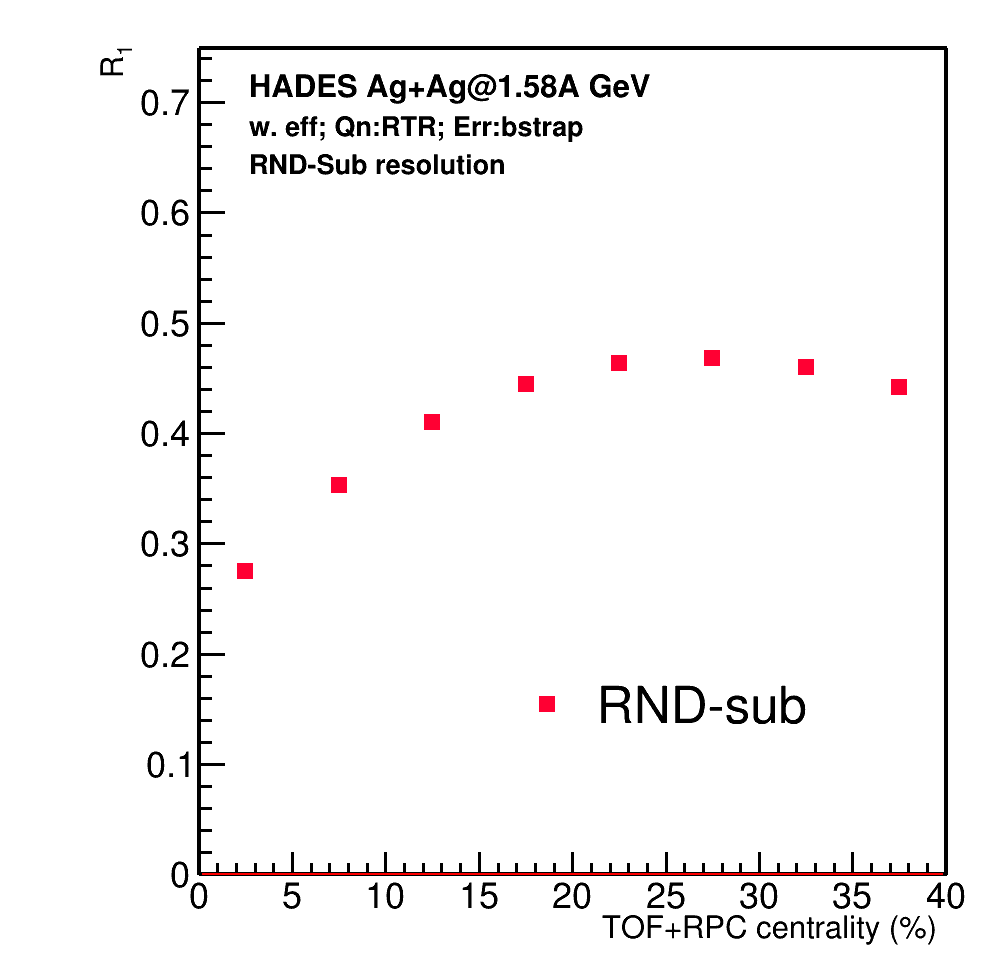
\includegraphics[width=0.3\linewidth]{images/R1_ag158_rnd_centrality.png}
    \caption{Разрешение плоскости симметрии рассчитанное методом случайных подсобытий как функция центральности столкновения.
    Слева: для столкновений Au + Au при $E_{kin}$=1.23$A$~ГэВ;
    посередине: для столкновений Ag + Ag при $E_{kin}$=1.23$A$~ГэВ; 
    справа: для столкновений Ag + Ag при $E_{kin}$=1.58$A$~ГэВ; 
    }
    \label{fig:hades_R1_rs}
\end{center}
\end{figure}
%

Для расчета разрешения методом трёх подсобытий в работе введены 5 $Q_1$-векторов. 
Используя в методе трех подсобытий различные комбинации векторов, можно оценить остаточные эффекты из-за непотоковых корреляций. 
Очевидно, что разрешение плоскости симметрии, посчитанное с использованием различных комбинаций, должны совпадать, а возможная разница будет связана с эффектами не относящимися к коллективному движению частиц.
Исключая из анализа разрешение полученное при помощи комбинаций, в которых два или более векторов коррелируют по непотоковому каналу, можно значительно уменьшить вклад непотоковых корреляций в полученные результаты.
Таким образом, систематическая ошибка из-за эффектов, не связанных с коллективным движением частиц может быть рассчитана следующим образом:
\begin{equation}
    \delta_{NF} = R_1\{a(b,c)\} - R_1\{d(e,f)\},
\end{equation}
где $\delta_{NF}$ --- ошибка из-за непотоковых корреляций, а буквами от $a$ до $f$ обозначены различные $Q_1$-вектора.

Разрешение плоскости симметрии $W1$, полученное с использованием различных комбинаций $Q_1$-векторов, показано на рис~\ref{fig:hades_w1_combinations}.
Разрешение $R_1\{W1(W2,W3)\}$ заметно отличается от значений, полученных при помощи других комбинаций. 
Этот эффект может быть объяснён наличием непотоковых корреляций между парами $Q_1$-векторов $W1$ и $W2$, $W2$ и $W3$.
Эти векторы не имеют достаточного разделения по быстроте, поэтому в значительной степени могут быть подвержены непотоковым корреляциям. 
В столкновениях Ag+Ag при обеих энергиях, $R_1\{W1(Mf,Mb)\}$ также значительно отклоняется от среднего результата. 
Это может быть вызвано наличием корреляций из-за закона сохранения импульса между векторами $Mf$ и $Mb$. 
В столкновениях Au+Au этот эффект менее выражен в силу большей множественности рождённых частиц.
%
\begin{figure}[ht]
\begin{center}
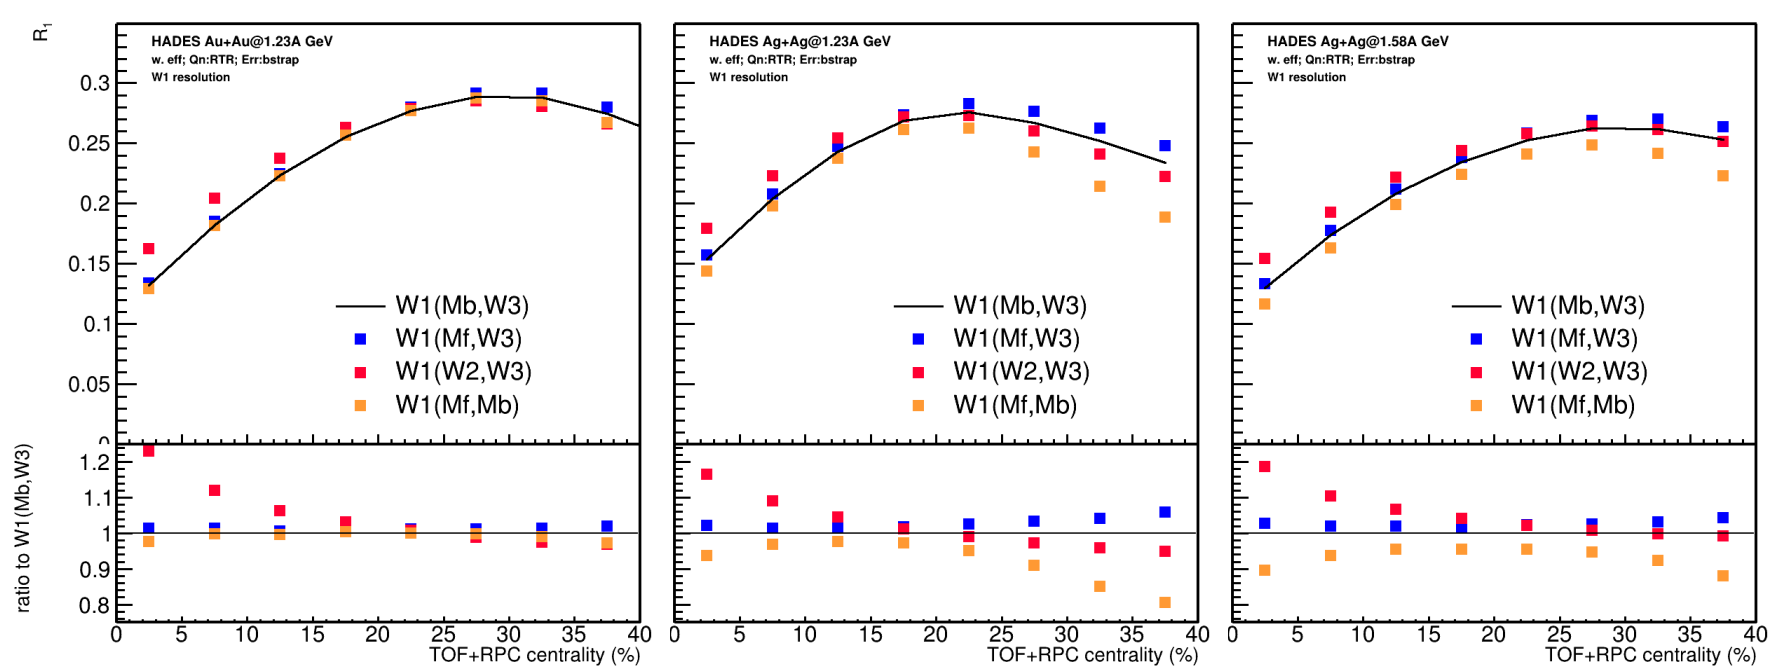
\includegraphics[width=0.75\linewidth]{images/W1_combinations.png}
\caption{Сравнение разрешений плоскости симметрии $W1$ полученное с использованием различных комбинаций $Q_1$-векторов для Au+Au@1.23A ГэВ (слева), Ag+Ag@1.23A ГэВ (посередине) и Ag+Ag@1.58A ГэВ (справа)}
\label{fig:hades_w1_combinations}
\end{center}
\end{figure}

\section{Эксперимент BM@N}

\subsection{Моделирование отклика установки}

Разработанная физическая программа измерения коллективных потоков в эксперименте BM@N была проверена на реалистичном Монте-Карло моделировании отклика детектора. 
В качестве входных данных моделирования были использованы две физические модели столкновения тяжелых ионов.
Модель DCM-QGSM-SMM (Dubna Cascade Model, Quark-Gluon String Model, Statistical Multifragmentation Model)~\cite{Botvina:1994vj,Baznat:2019iom} реалистично описывает выход спектаторных фрагментов, однако неудовлетворительно воспроизводит коллективную анизотропию рожденных частиц.
Эта модель была использована для проверки разработанных методов вычисления поправочного коэффициента разрешения в эксперименте BM@N.

Модель JAM (Jet-A-A Model)~\cite{Nara:2016hbg,Nara:2019qfd,Nara:2020ztb} с импульсно-зависимым потенциалом дает реалистичный сигнал коллективной анизотропии рожденных барионов, однако в модели отсутствуют фрагменты с массовым номером $A>1$.
Данная модель была использована для проверки коррекций на неоднородность детектора и возможности алгоритмов реконструкции восстановить сигнал коллективной анизотропии.

\subsection{Определение центральности}

В эксперименте BM@N центральность также была определена при помощи метода Монте-Карло Глаубера, однако в качестве множественности использовалось число восстановленных траекторий заряженных частиц~\cite{Segal:2023njv}.
На рис.~\ref{fig:bmn_multiplicity} представлено распределение множественности заряженных частиц для Монте-Карло моделирования столкновений Xe+Cs(I) при энергии $E_{kin}$=4$A$~ГэВ.
Вертикальными линиями обозначены границы классов центральности.
Модель Монте-Карло Глаубера хорошо описывает распределение множественности в границах 0-60\% класса центральности.
%
\begin{figure}[ht]
\begin{center}
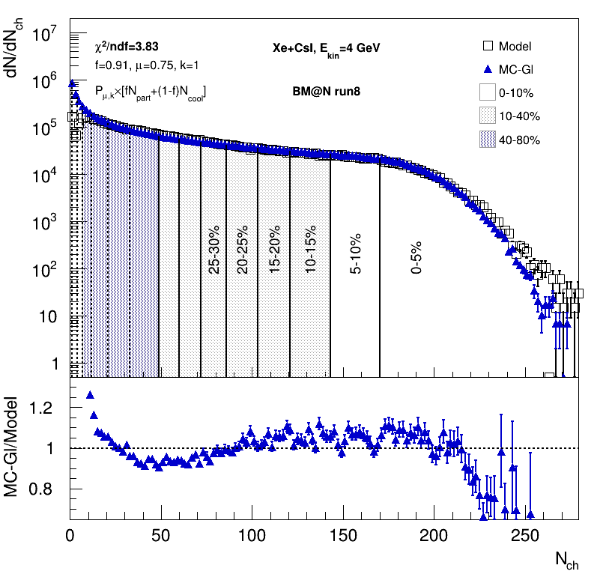
\includegraphics[width=0.75\linewidth]{images/bmn_multiplicity.png}
\caption{Распределение множественности заряженных частиц в эксперименте BM@N. Вертикальными линиями изображены границы классов центральности.}
\label{fig:bmn_multiplicity}
\end{center}
\end{figure}

\subsection{Идентификация протонов}

Для каждого из детекторов была построена зависимость квадрата массы делённого на квадрат заряда $m^2/q^2$ от импульса $p/q$. 
На рис.~\ref{fig:bmn_m2_pq} сверху, представлено распределение квадрата массы заряженной частицы в зависимости от импульса $p/q$ для TOF-400 (слева) и TOF-700 (справа).
В узких диапазонах поперечного импульса распределение частиц по квадрату массы было аппроксимировано гауссовой функцией. 
На рис.~\ref{fig:bmn_m2_pq} снизу, представлены кандидаты в протоны, которые лежат не дальше $2\sigma$ от пика квадрата массы.
%
\begin{figure}[ht]
\begin{center}
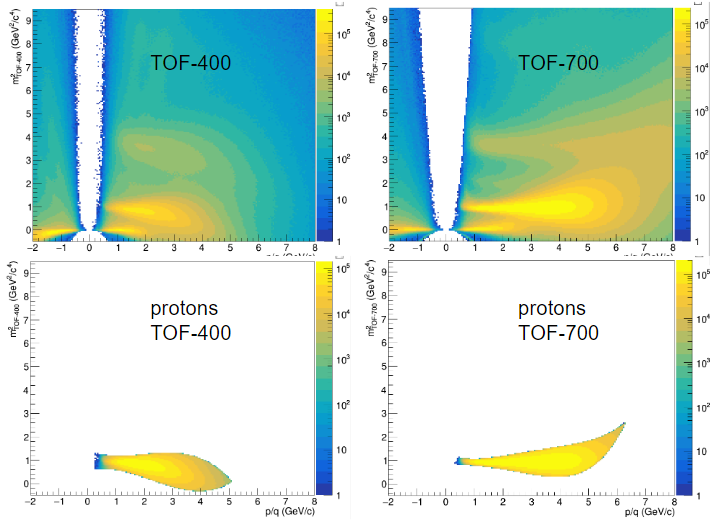
\includegraphics[width=0.95\linewidth]{images/bmn_m2_pq.png}
\caption{Распределение квадрата массы деленного на квадрат заряда заряженной частицы в зависимости от импульса $p/q$ для TOF-400 (слева) и TOF-700 (справа). Сверху представлены распределения для всех заряженных частиц, снизу --- для отобранных протонов.}
\label{fig:bmn_m2_pq}
\end{center}
\end{figure}


На рис.~\ref{fig:bmn_pt_y} представлено распределение протонов по быстроте $y_{cm}$ и поперечному импульсу $p_T$ идентифицированных при помощи TOF-400 (слева сверху), TOF-700 (слева снизу), с использованием обоих TOF-детекторов (справа).
%
\begin{figure}[ht]
\begin{center}
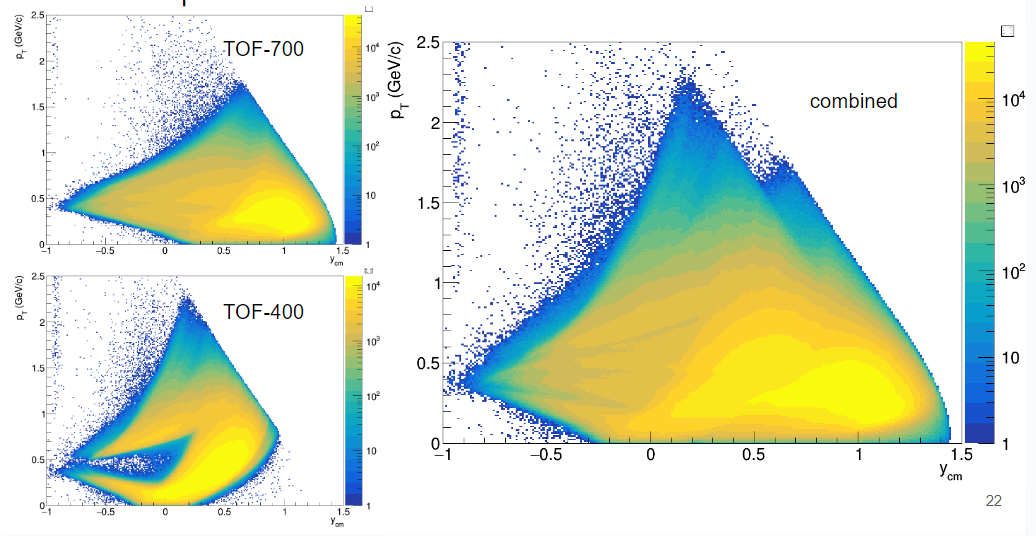
\includegraphics[width=0.95\linewidth]{images/bmn_pt_y_acceptance.png}
\caption{Распределение протонов по быстроте $y_{cm}$ и поперечному импульсу $p_T$, идентифицированных при помощи TOF-400 (слева сверху), TOF-700 (слева снизу), с использованием обоих TOF-детекторов (справа).}
\label{fig:bmn_pt_y}
\end{center}
\end{figure}


\subsection{Кинематические окна, в которых были определены $Q_1$-вектора}

Для восстановления плоскости симметрии в эксперименте BM@N была использована информация с калориметра FHCal.
Модули детектора были разделены на 3 группы согласно их псевдобыстроте (F1, F2 и F3).
Схематические группы модулей изображены различными цветами на рис.~\ref{fig:bmn_subevents} слева.

Дополнительно для исследования вклада непотоковых корреляций в измеренные значения коллективной анизотропии были введены два $Q_1$-вектора из треков заряженных частиц. 
Вектор $Tp$ построен для протонов со значениями быстроты $0.4<y_{cm}<0.6$ и поперечным импульсом $0.2<p_{T}<2.0$~$GeV/c$.
Вектор $T\pi$ формировался для отрицательных пионов с быстротой и поперечным импульсом $0.2<y_{cm}<0.8$ и $0.1<p_T<0.5 GeV/c$ соответственно.
Соответствующие кинематические области изображены красными прямоугольниками на рис.~\ref{fig:bmn_subevents} справа.
%
\begin{figure}[ht]
\begin{center}
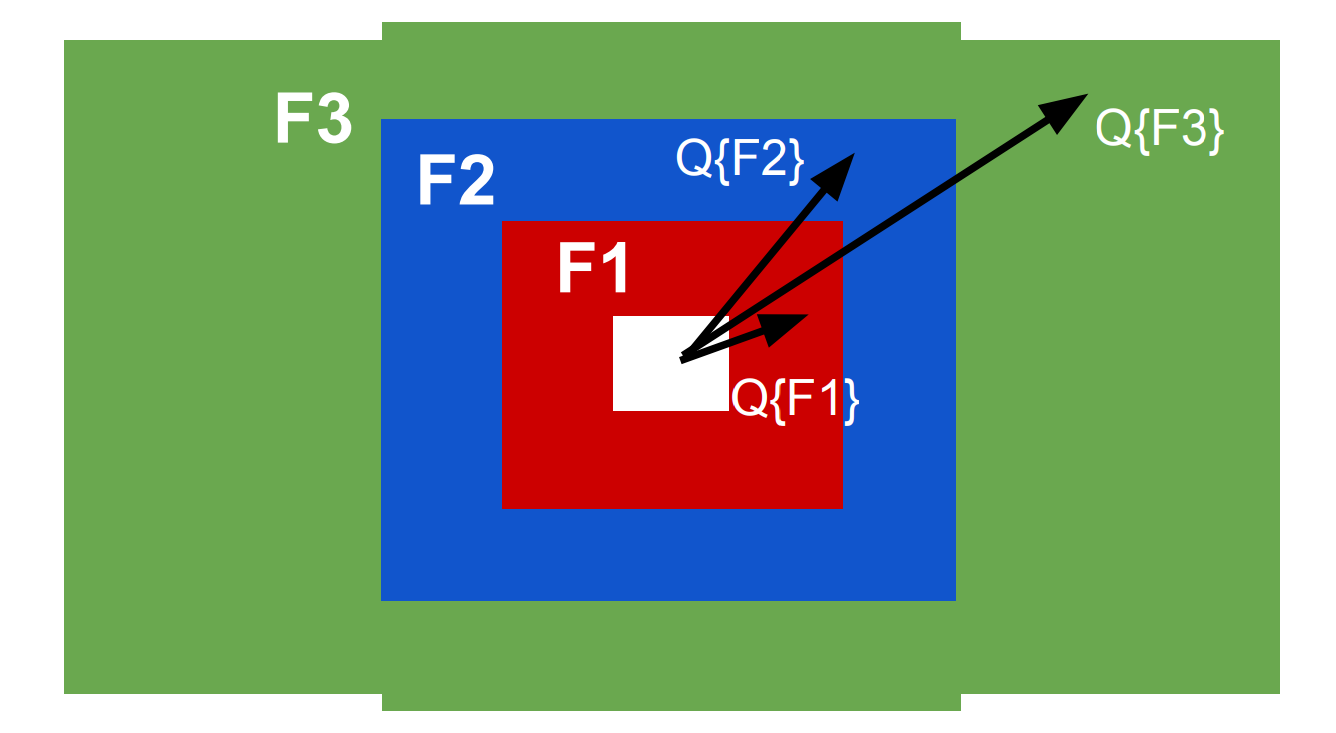
\includegraphics[width=0.45\linewidth]{images/FHCal_layout.png}
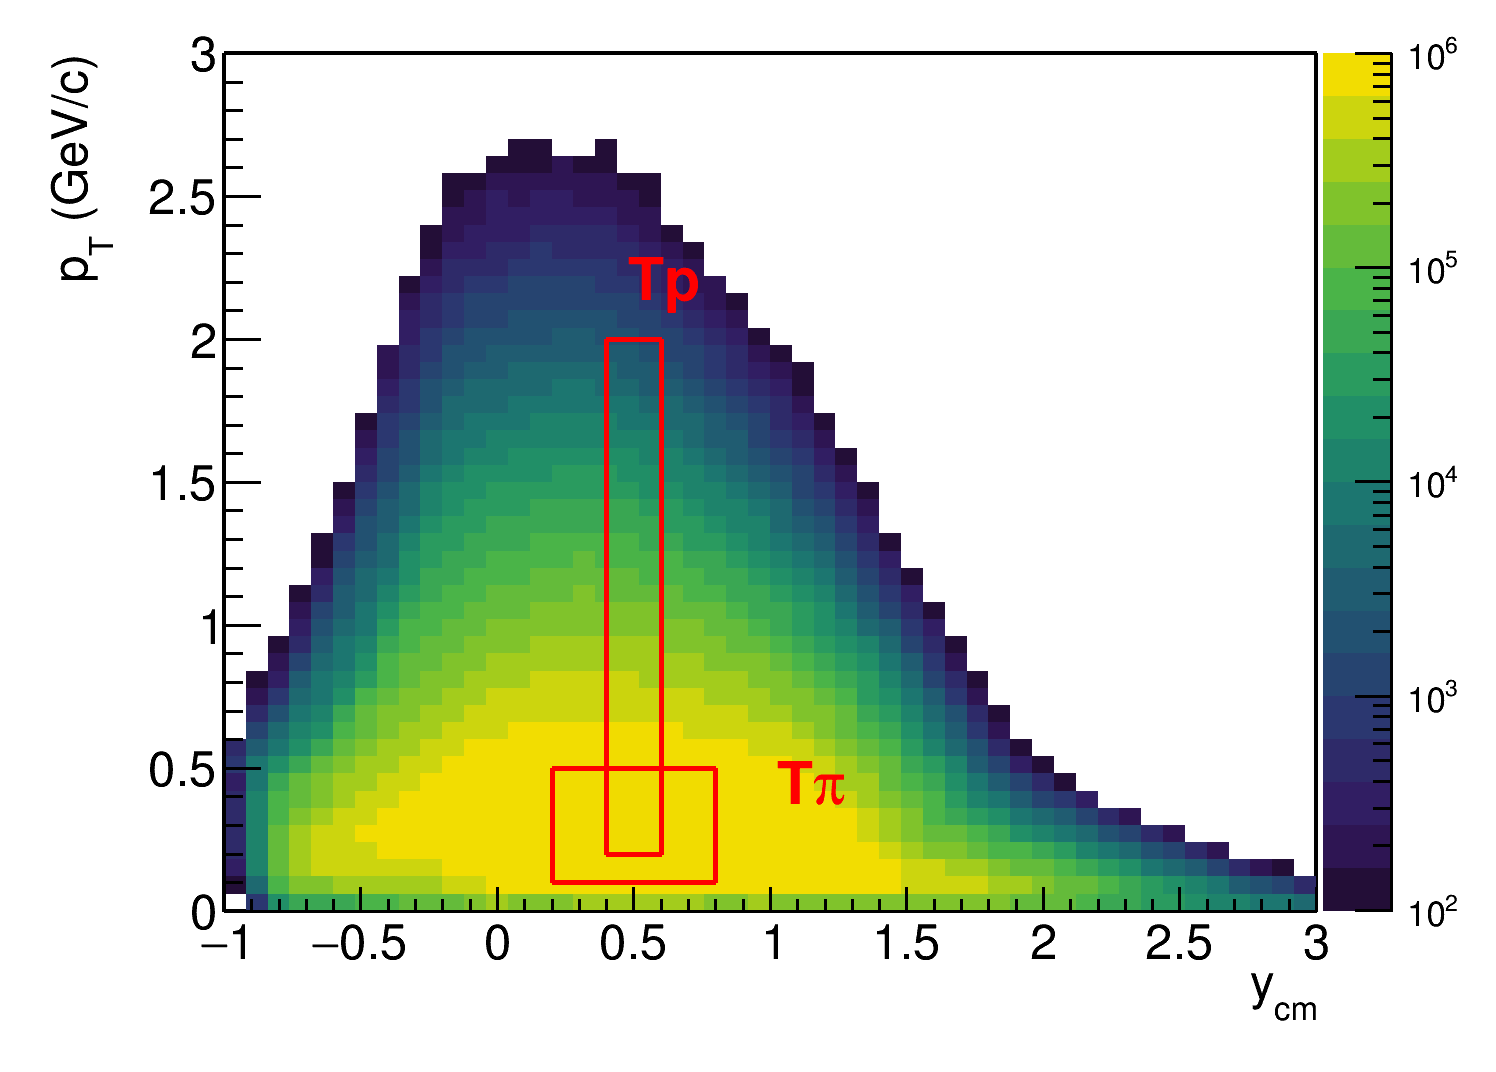
\includegraphics[width=0.45\linewidth]{images/pT_ycm_protons.png}
\caption{
Слева: Схема разделения модулей переднего адронного калориметра по группам для определения плоскости симметрии события.
Справа: Кинематические окна для подсчета $Q_1$-векторов из треков заряженных частиц.
}
\label{fig:bmn_subevents}
\end{center}
\end{figure}

\section{Выводы к главе 3}

В главе описаны методы определения центральности и идентификации протонов с помощью экспериментальной установки HADES.
Представлены критерии отбора столкновений Au+Au и Ag+Ag а также заряженных частиц, рожденных в этих столкновениях.
Описаны способы вычисления эффективности реконструкции протонов при помощи программного пакета GEANT3.
В главе обсуждаются методы определения плоскости симметрии столкновения а также способы вычисления разрешения плоскости симметрии при помощи переднего годоскопа FW в эксперименте HADES.
Приводятся результаты применения коррекций на азимутальную анизотропию аксептанса установки HADES и обсуждаются остаточные систематические погрешности, связанные с этим эффектом.

Для экспериментальной установки BM@N описываются методы измерения центральности столкновения по числу треков заряженных частиц. 
В главе обсуждаются способы измерения производительности установки BM@N для измерения направленного и эллиптического потоков протонов с помощью физических Монте-Карло моделей столкновений тяжелых ионов и программного пакета GEANT4.
В главе представлены значения поправочного коэффициента разрешения $R_1$ для плоскостей симметрии, определенных при помощи переднего годоскопа FW.
Обсуждаются методы минимизации систематической ошибки связанной с непотоковыми корреляциями и вычисляется остаточная систематическая ошибка.
В главе представлены кинематические диапазоны, использованные для вычисления $Q_1$-векторов в Монте-Карло симуляции эксперимента BM@N.           % Глава 3
\chapter{Результаты анализа коллективной анизотропии}

\section{Результаты анализа экспериментальных данных HADES}

\section{Оценка вклада непотоковых корреляций в значения поправочного коэффициента разрешения $R_1$}

Для оценки систематики из-за непотоковых корреляций в полученных результатах $v_1$, был использован аналогичный метод, что и для разрешения плоскости симметрии. 
Для каждой плоскости симметрии, направленный поток может быть скорректирован на поправочный коэффициент разрешения рассчитанный с использованием различных комбинаций $Q_1$-векторов.
Сравнивая значения поправочного коэффициента, полученного при помощи различных комбинаций, можно оценить вклад непотоковых корреляций между $Q_1$-векторами.
Для проверки величины непотоковых корреляций между векторами частиц $u_1$ и вектором плоскости симметрии $Q_1$, можно сравнить значения $v_1$, полученные относительно различных плоскостей симметрии.
Таким образом, сравнивая направленный поток $v_1$, полученный относительно различных плоскостей симметрии и деленный на поправочный коэффициент разрешения, вычисленный с использованием различных комбинаций $Q_1$-векторов можно оценить вклад непотоковых корреляций в измеренные значения $v_1$.

На рис.~\ref{fig:hades_w1w3} представлен направленный поток протонов $v_1$, рожденных в столкновении Au+Au при энергии $E_{kin}=$1.23$A$~ГэВ, как функция центральности столкновения, измеренный относительно различных $Q_1$-векторов. 
Коррекция на поправочный коэффициент разрешения выполнена с использованием различных комбинаций $Q_1$-векторов.
Слева представлены значения $v_1$ протонов измеренные относительно внутреннего подсобытия W1, справа --- внешнего подсобытия W3 и подсобытия из треков заряженных частиц Mf. 
Результаты для комбинаций подсобытий, разделенных по быстроте, таких как например, $W1(Mf,W3)$ и $W1(Mb,W3)$ согласуются между собой в пределах 2\%, за исключением наиболее центральных событий. 
Результаты для $v_1$, полученные с использованием комбинации не разделенных по быстроте $Q_1$-векторов (например $W1(W2,W3)$) значительно отличаются.
Направленный поток протонов $v_1$, измеренный относительно различных плоскостей симметрии $W1$ и $W3$, так же согласуется в пределах 2\%.
Значения $v_1$ протонов, полученные относительно треков заряженных частиц $Mf$, систематически отличается от результатов полученных относительно плоскостей $W1$ и $W3$. 
Отсюда можно сделать вывод о недостаточном разделении по быстроте между подсобытием $Mf$ и рожденными протонами, для которых производились измерения.
В то же самое время, разделение по быстроте между зарегистрированными протонами и подсобытиям $W1$ и $W3$ достаточно.
В дальнейшем, в качестве значений $v_1$ протонов будет использовано среднее по всем комбинациям $Q_1$-векторов, разделенных по быстроте.
%
\begin{figure}[ht]
\begin{center}
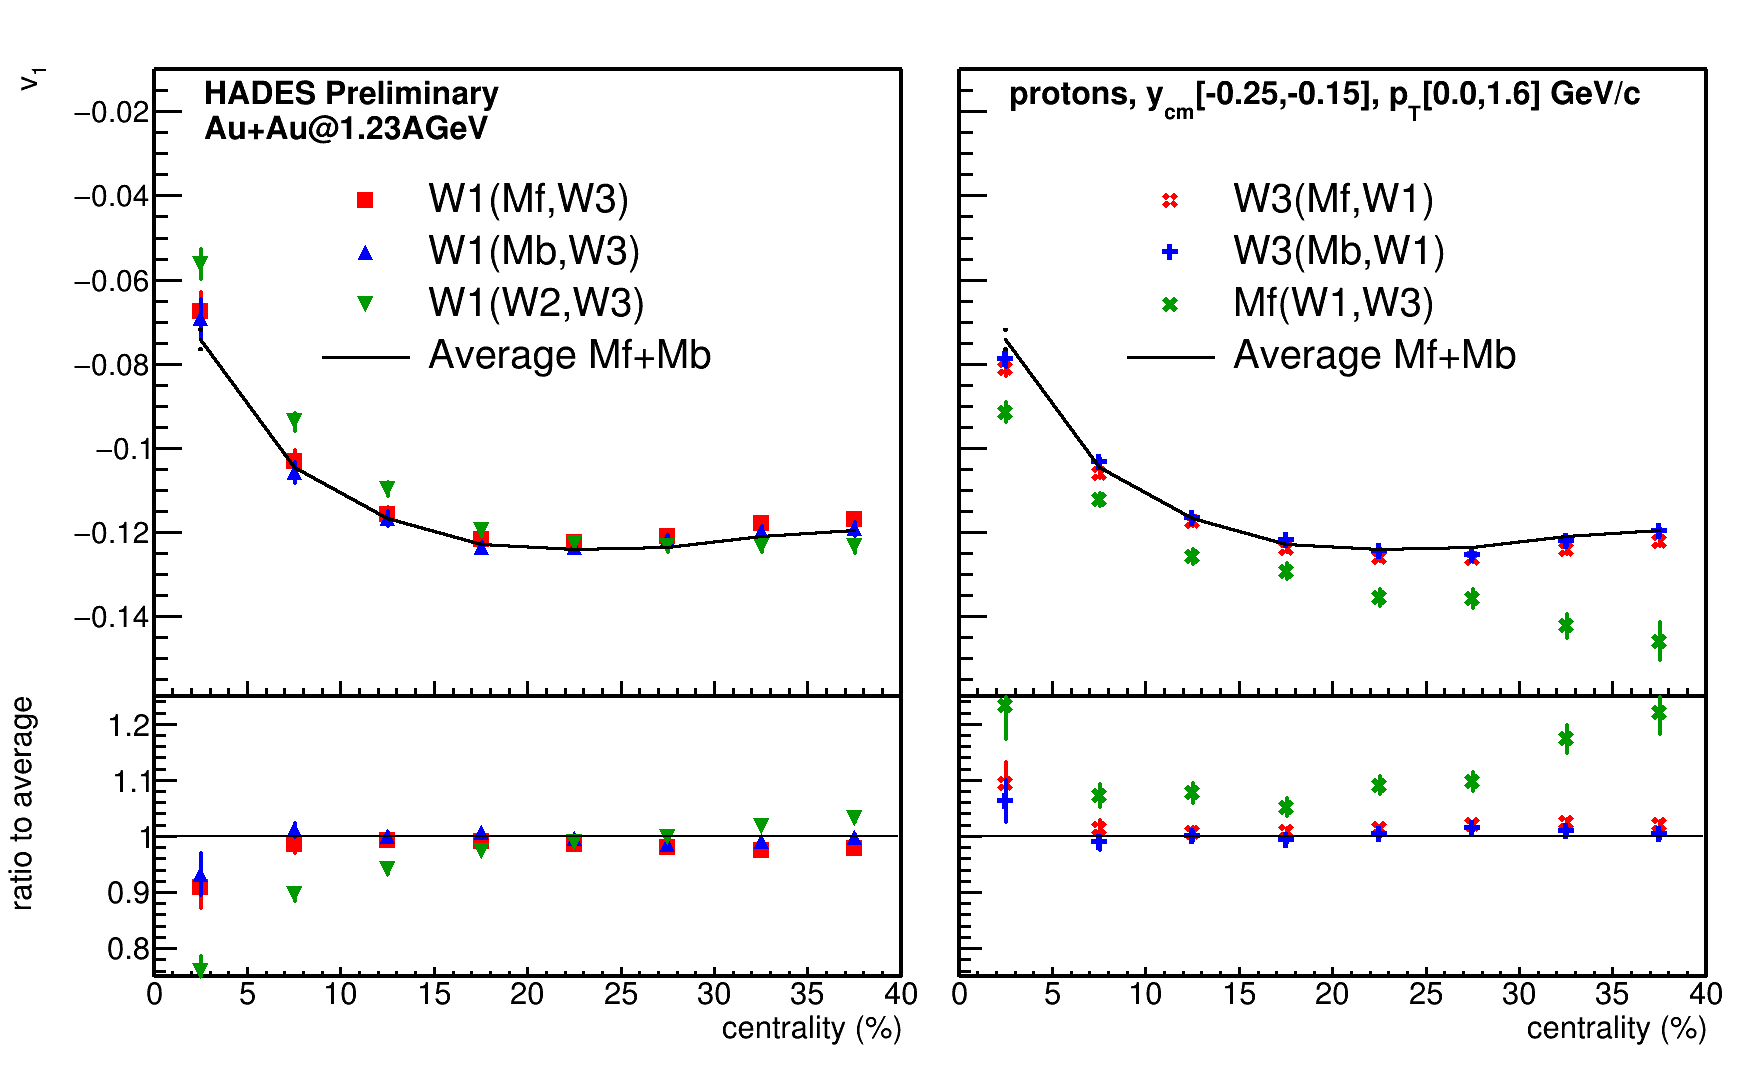
\includegraphics[width=0.75\linewidth]{images/W1AndW3Nucleus.png}
\caption{Направленный поток протонов $v_1$ рожденных в столкновении Au+Au при энергии $E_{kin}=$1.23$A$~ГэВ как функция центральности столкновения, измеренный при помощи различных комбинаций $Q_1$-векторов. Слева представлены значения $v_1$ протонов измеренные относительно внутреннего подсобытия W1, справа --- внешнего подсобытия W3 и подсобытия из треков заряженных частиц Mf. Черной линией представлено среднее результатов полученных при помощи разделенных по быстроте комбинаций.}
\label{fig:hades_w1w3}
\end{center}
\end{figure}

\subsection{Сравнение методов плоскости события и скалярного произведения}

Измерения направленного потока в~\cite{HADES:2020lob} были выполнены используя метод плоскости события. 
Для оценки возможной систематики, связанной с этим методом измерения $v_1$, направленный поток был рассчитан также методом скалярного произведеления.
Сравнение результатов полученных этими двумя методами позволит оценить вклад нелинейной зависимости $v_1\{EP\}$ от аксептанса установки и реального значения $v_1$.

На рисунке~\ref{fig:hades_ep_vs_sp} представлен направленный поток протонов рожденных в столкновениях Au+Au при энергии $E_{kin}=$1.23$A$~ГэВ как функция центральности, измеренный методом плоскости события и скалярного произведения. 
Значения $v_1$, полученные различными методами, хорошо согласуются между собой с учетом статистической ошибки. 
%
\begin{figure}[ht]
\begin{center}
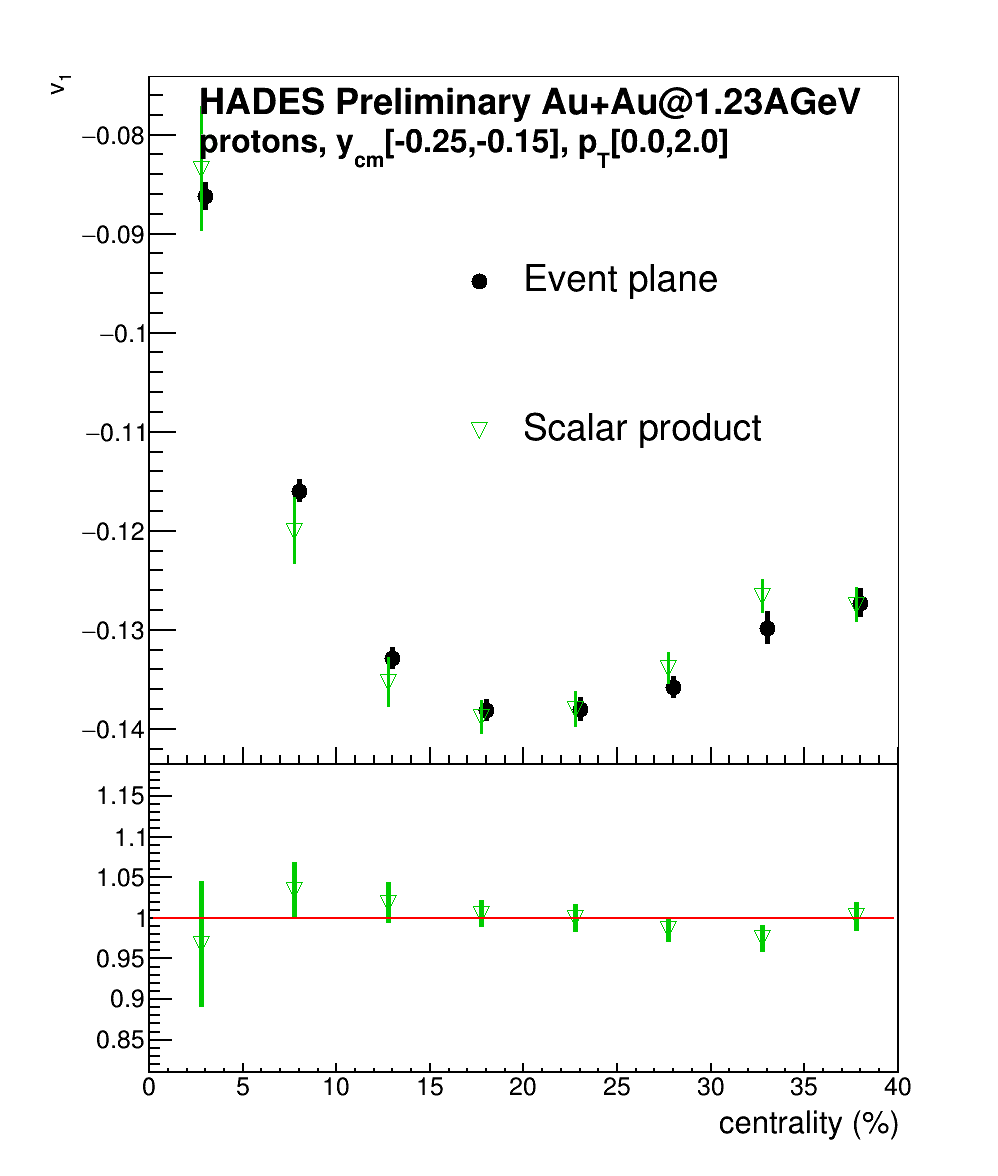
\includegraphics[width=0.45\linewidth]{images/EP_vs_SP.png}
\caption{Направленный поток протонов $v_1$, рожденных в столкновении Au+Au при энергии $E_{kin}=$1.23$A$~ГэВ как функция центральности столкновения. Результаты показаны для методов скалярного произведения (SP) и плоскости события (EP).}
\label{fig:hades_ep_vs_sp}
\end{center}
\end{figure}

\subsection{Сравнение методов случайных подсобытий и метода трёх подсобытий}

На рис.~\ref{fig:hades_rs_3s} показан направленный поток $v_1$ протонов, рожденных в столкновении Au+Au при энергии $E_{kin}=$1.23$A$~ГэВ (слева), Ag + Ag при энергии $E_{kin}=$1.23$A$~ГэВ (посередине) и Ag + Ag при энергии $E_{kin}=$1.58$A$~ГэВ (справа) как функция центральности столкновения. Результаты представлены для методов трех подсобытий и метода случайных подсобытий.
Для столкновений Au + Au при при энергии $E_{kin}=$1.23$A$~ГэВ (слева) разница между двумя методами вычисления корректировочного коэффициента разрешения составляет менее 5\% для среднецентральных столкновений.
Однако для меньшей системы столкновения, разница значительно больше. 
Это может быть объяснено меньшей множественностью рожденных частиц и спектаторов, и большим относительным вкладом непотоковых корреляций между $Q_1$-векторами, используемыми для расчета разрешения плоскости симметрии.
Наибольшая разница между двумя методами наблюдается для столкновений Ag + Ag при энергии $E_{kin}=$1.58$A$~ГэВ (справа).
Этот факт объясняется меньшим значением направленного потока $v_1$ спектаторов, отсюда больший относительный вклад непотоковых корреляций.
На основании этого наблюдения, можно сделать вывод о ненадёжности метода случайных подсобытий для более лёгких систем.
%
\begin{figure}[ht]
\begin{center}
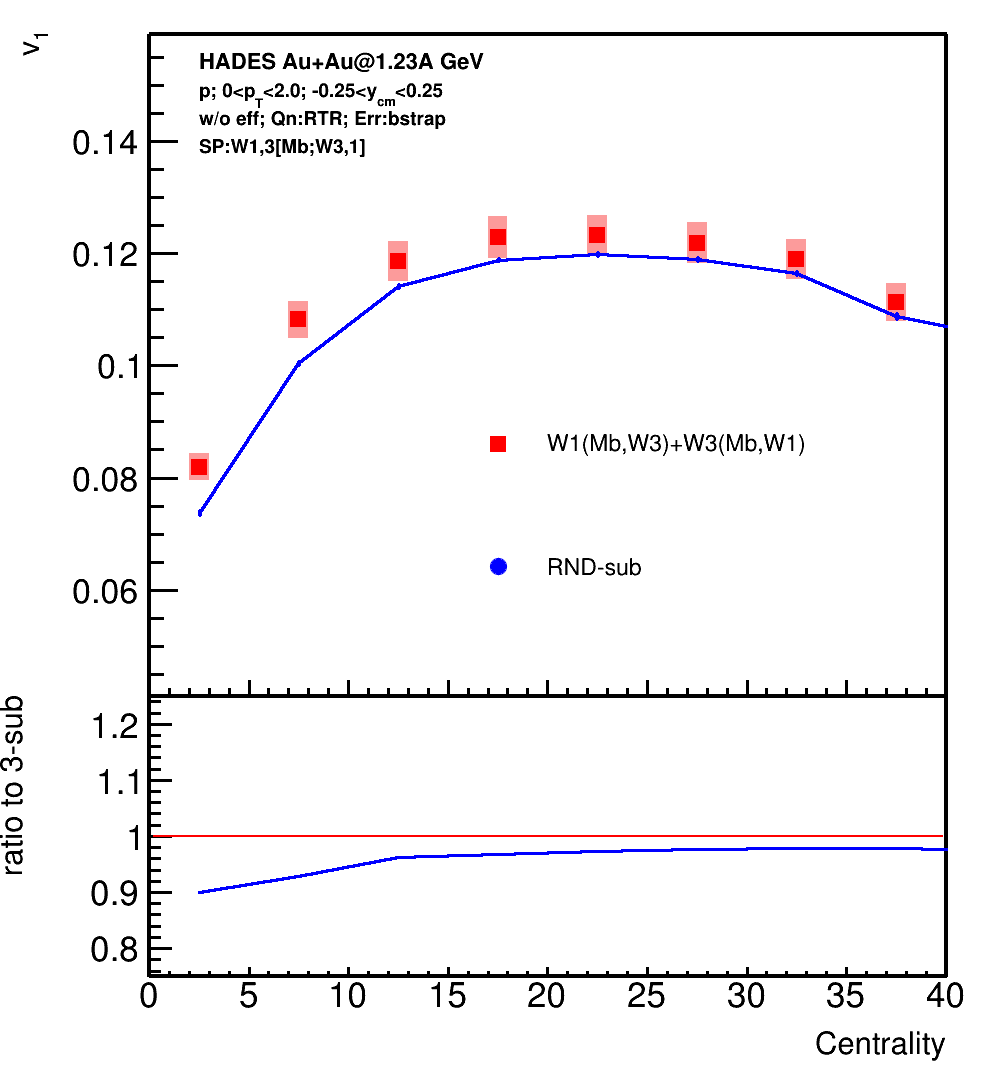
\includegraphics[width=0.3\linewidth]{images/v1_au123_3s_rnd.png}
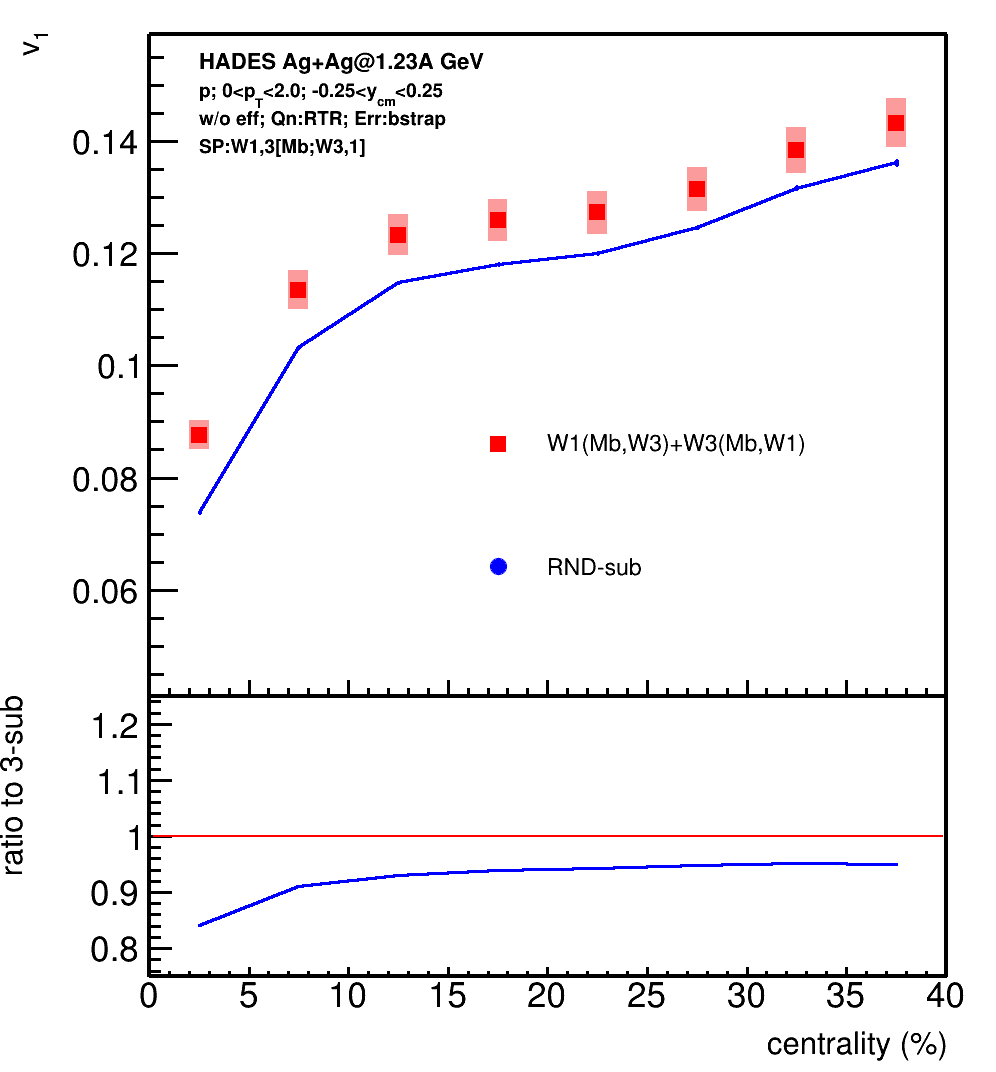
\includegraphics[width=0.3\linewidth]{images/v1_ag123_3s_rnd.png}
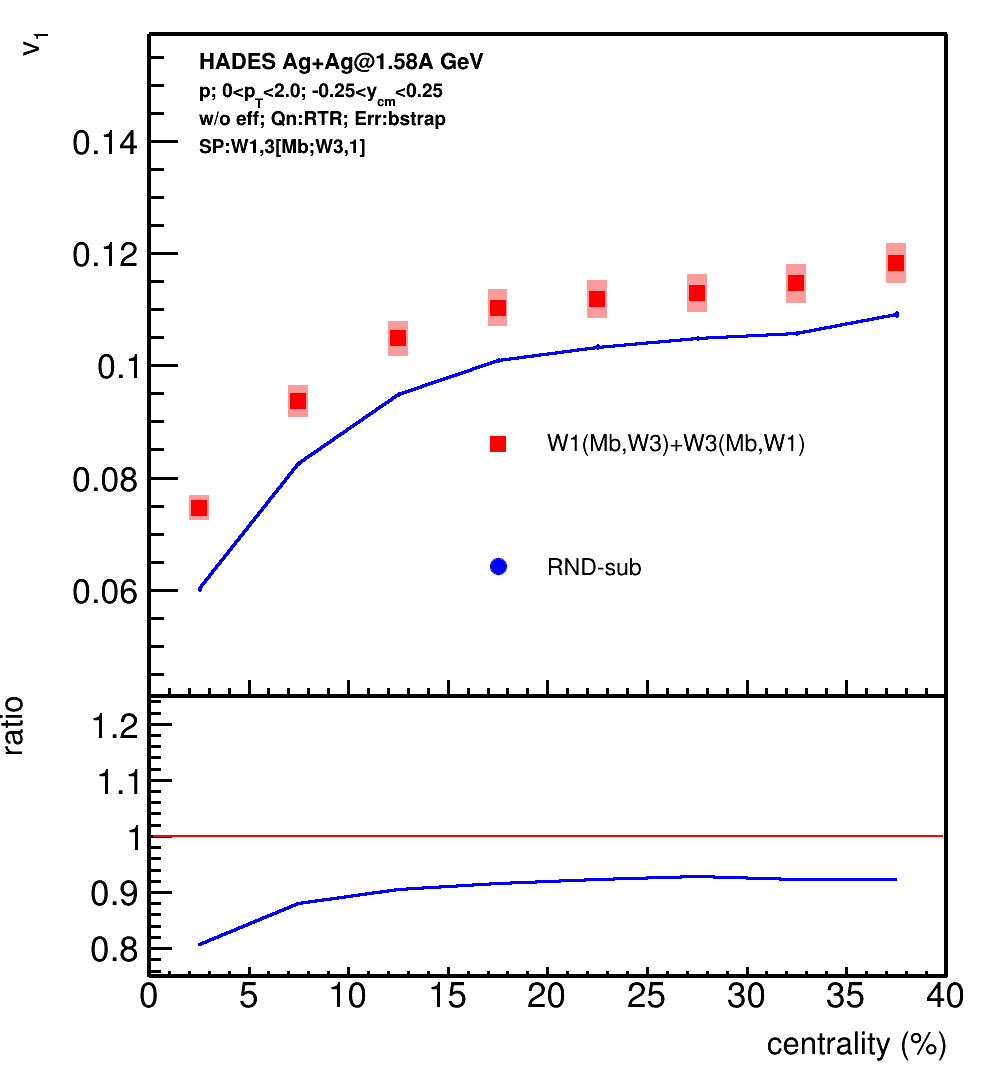
\includegraphics[width=0.3\linewidth]{images/v1_ag158_3s_rnd.png}
\caption{Направленный поток $v_1$ протонов, рожденных в столкновении Au+Au при энергии $E_{kin}=$1.23$A$~ГэВ (слева), Ag + Ag при энергии $E_{kin}=$1.23$A$~ГэВ (посередине) и Ag + Ag при энергии $E_{kin}=$1.58$A$~ГэВ (справа) как функция центральности столкновения. Результаты показаны для методов трех подсобытий и метода случайных подсобытий.}
\label{fig:hades_rs_3s}
\end{center}
\end{figure}

\subsection{Оценка итоговой систематики в значения $v_1$ от непотоковых корряляций}

На основании этих результатов, был сделан вывод о малом вкладе непотоковых корреляций в итоговые значения $v_n$ протонов и лёгких ядер, измеренных на установке HADES. 
Эти результаты легли в основу систематической ошибки измерений коллективной анизотропии и позволили опубликовать полученные данные~\cite{HADES:2020lob}.
На рис.~\ref{fig:hades_prl} приведен направленный поток $v_1$ протонов рожденных в столкновениях ядер золота при кинетической энергии пучка $E_{kin}=1.23A$~ГэВ как функция быстроты и поперечного импульса.
%
\begin{figure}[ht]
\begin{center}
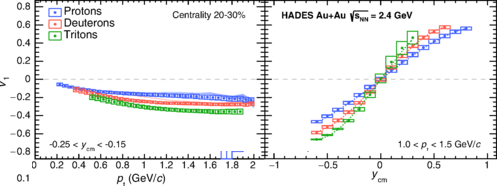
\includegraphics[width=0.75\linewidth]{images/HADES_prl.png}
\caption{Направленный поток ($v_1$) протонов, дейтронов и тритонов  рожденных в столкновении Au+Au при энергии $E_{kin}=$1.23$A$~ГэВ как функция быстроты (справа) и поперечного импульса (слева).}
\label{fig:hades_prl}
\end{center}
\end{figure}

\subsection{Сравнение результатов для $v_1$ протонов с опубликованными данными}

На рис.~\ref{fig:hades_v1_publ_comparison} представлено сравнение направленного потока измеренного для столкновений Au + Au при энергии $E_{kin}$=1.23$A$~ГэВ с опубликованными данными~\cite{HADES:2020lob}.
Направленный поток $v_1$ как функция быстроты (слева) и поперечного импульса (справа) хорошо согласуется с опубликованной зависимостью для протонов.
%
\begin{figure}[ht]
\begin{center}
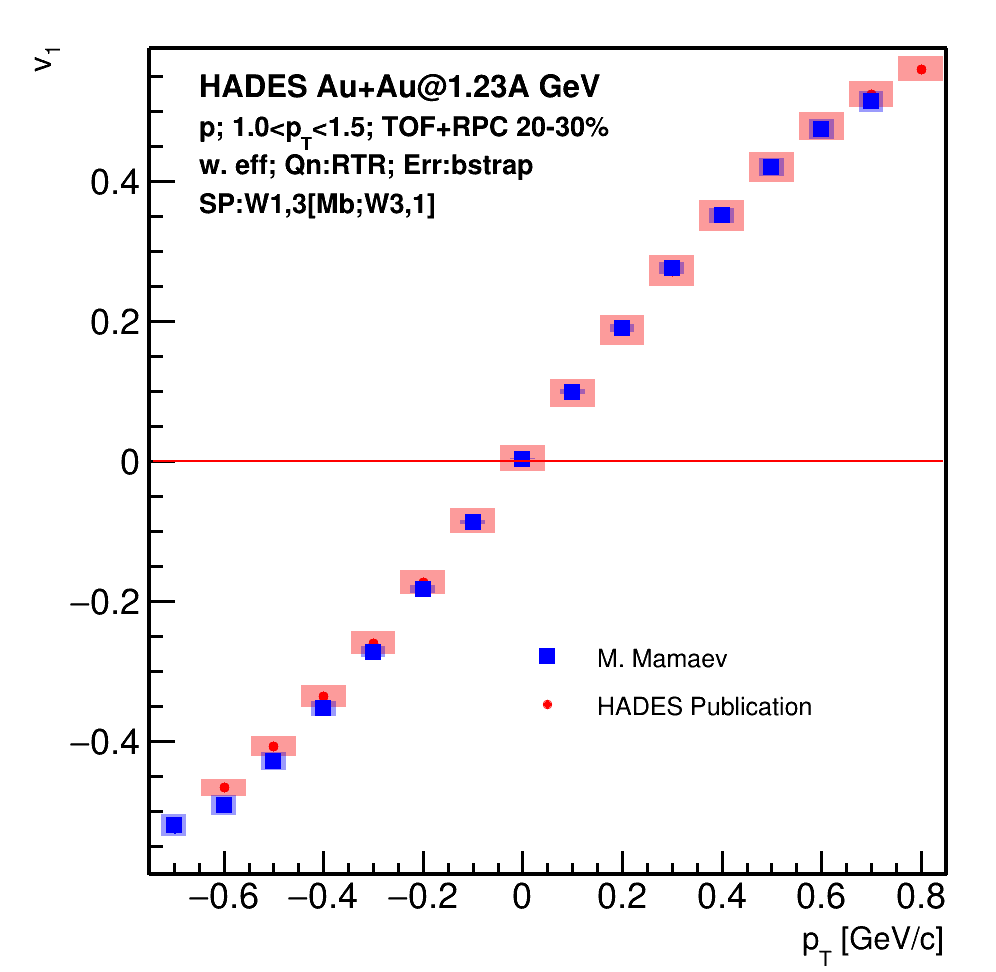
\includegraphics[width=0.45\linewidth]{images/v1_au123_publication_ycm.png}
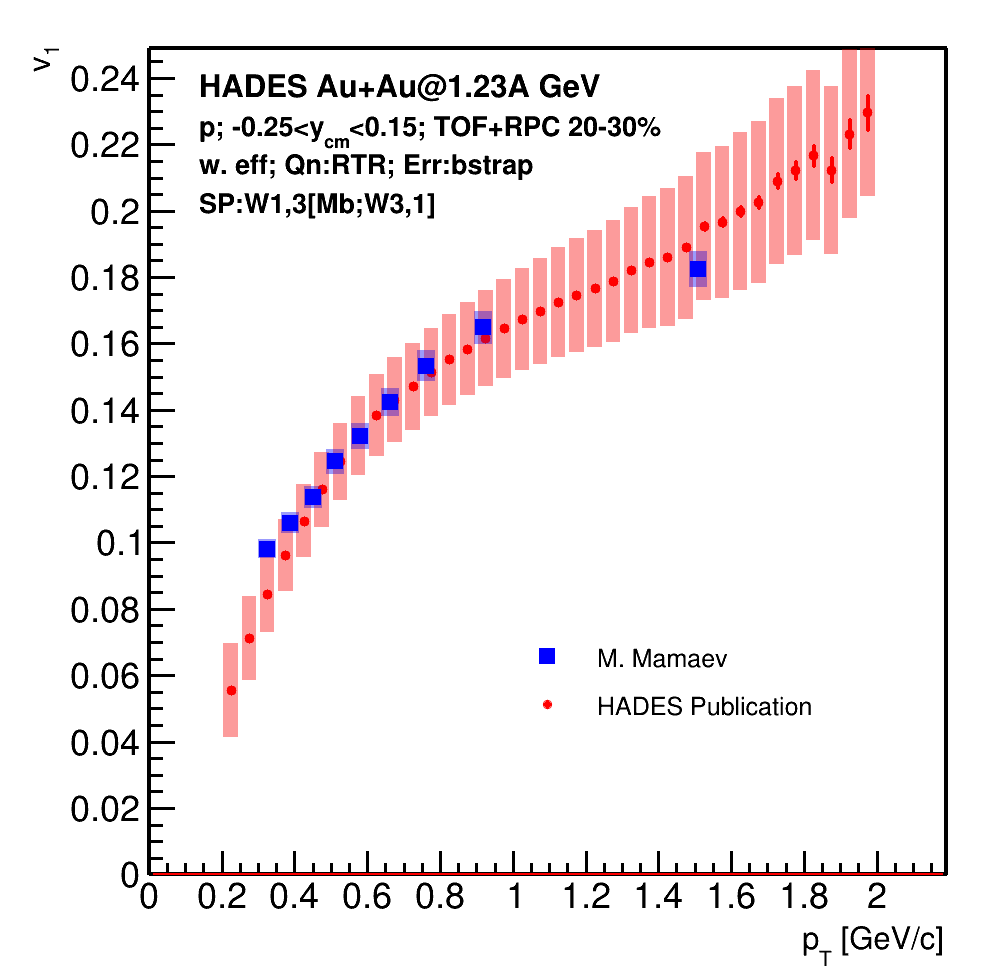
\includegraphics[width=0.45\linewidth]{images/v1_au123_publication_pT.png}
\caption{Направленный поток ($v_1$) протонов  рожденных в столкновении Au+Au при энергии $E_{kin}=$1.23$A$~ГэВ как функция быстроты (справа) и поперечного импульса (слева). Сравнение полученных результатов с опубликованными данными~\cite{HADES:2020lob}. }
\label{fig:hades_v1_publ_comparison}
\end{center}
\end{figure}

\subsection{Направленный поток $v_1$ протонов как функции быстроты и поперечного импульса в столкновениях Au + Au и Ag + Ag}

На рисунке~\ref{fig:hades_v1_ycm_pT} представлен направленный поток протонов $v_1$ как функция (слева) быстроты в системе центра масс $y_{cm}$ и (справа) поперечного импульса $p_T$ для столкновений Au+Au при энергии $E_{kin}=$1.23$A$~ГэВ и Ag+Ag при энергиях $E_{kin}=$1.23$A$ и 1.58$A$~ГэВ.
Значения $v_1$ протонов, в столкновениях Au+Au и Ag+Ag при одной энергии, хорошо согласуются с учетом систематической ошибки. 
Протоны, рожденные в столкновениях Ag+Ag при большей энергии $E_{kin}=$1.58$A$~ГэВ обладают меньшим $v_1$, поскольку направленный поток чувствителен ко времени взаимодействия области перекрытия и остатков сталкивающихся ядер.
Чем меньше время взаимодействия (чем больше энергия столкновения) тем меньше итоговое значение направленного потока.

Модель JAM~\cite{nara2019jam} с импульсно зависимым потенциалом хорошо описывает магнитуду $v_1$ протонов и зависимость наблюдаемой от быстроты $y_{cm}$.
Однако модель не способна описать зависимость $v_1$ от поперечного импульса $p_T$.
%
\begin{figure}[ht]
\begin{center}
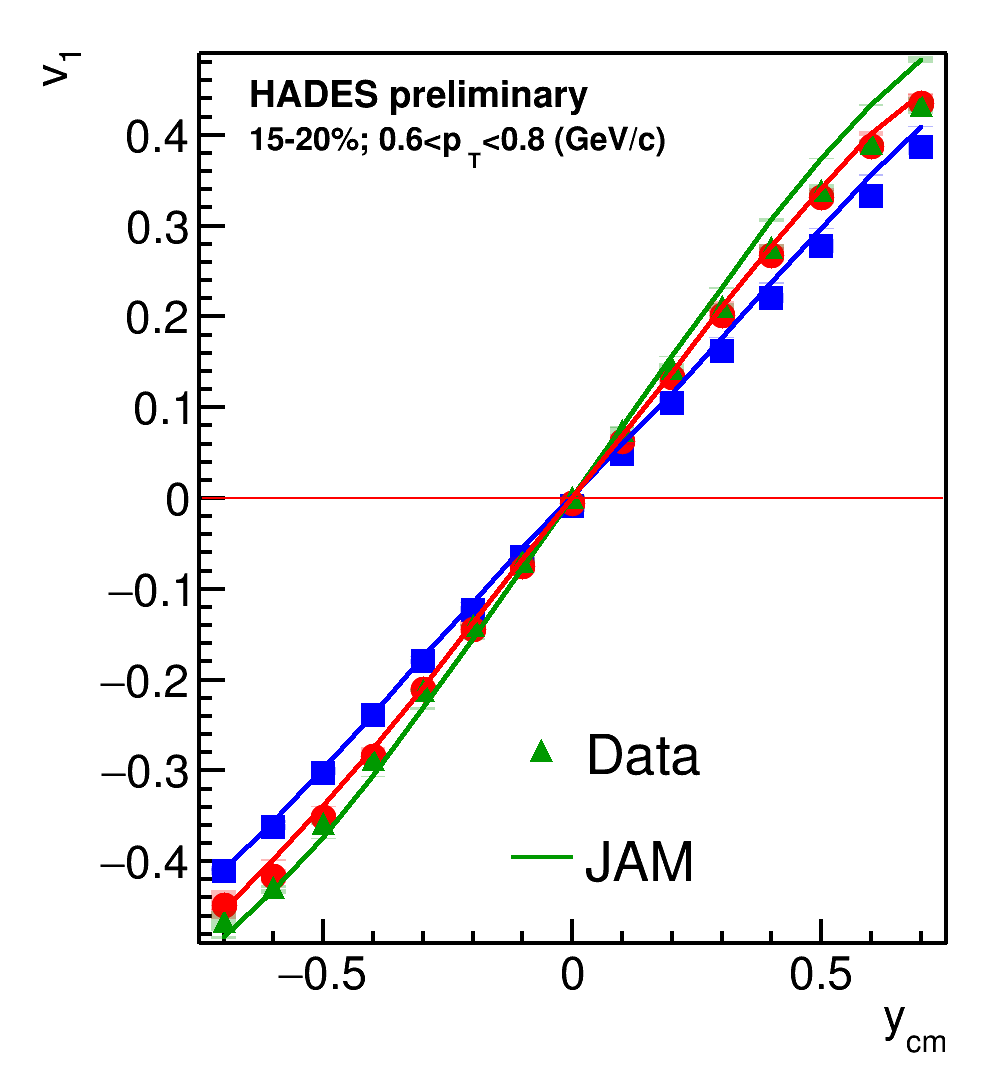
\includegraphics[width=0.45\linewidth]{images/v1_hades_ycm.png}
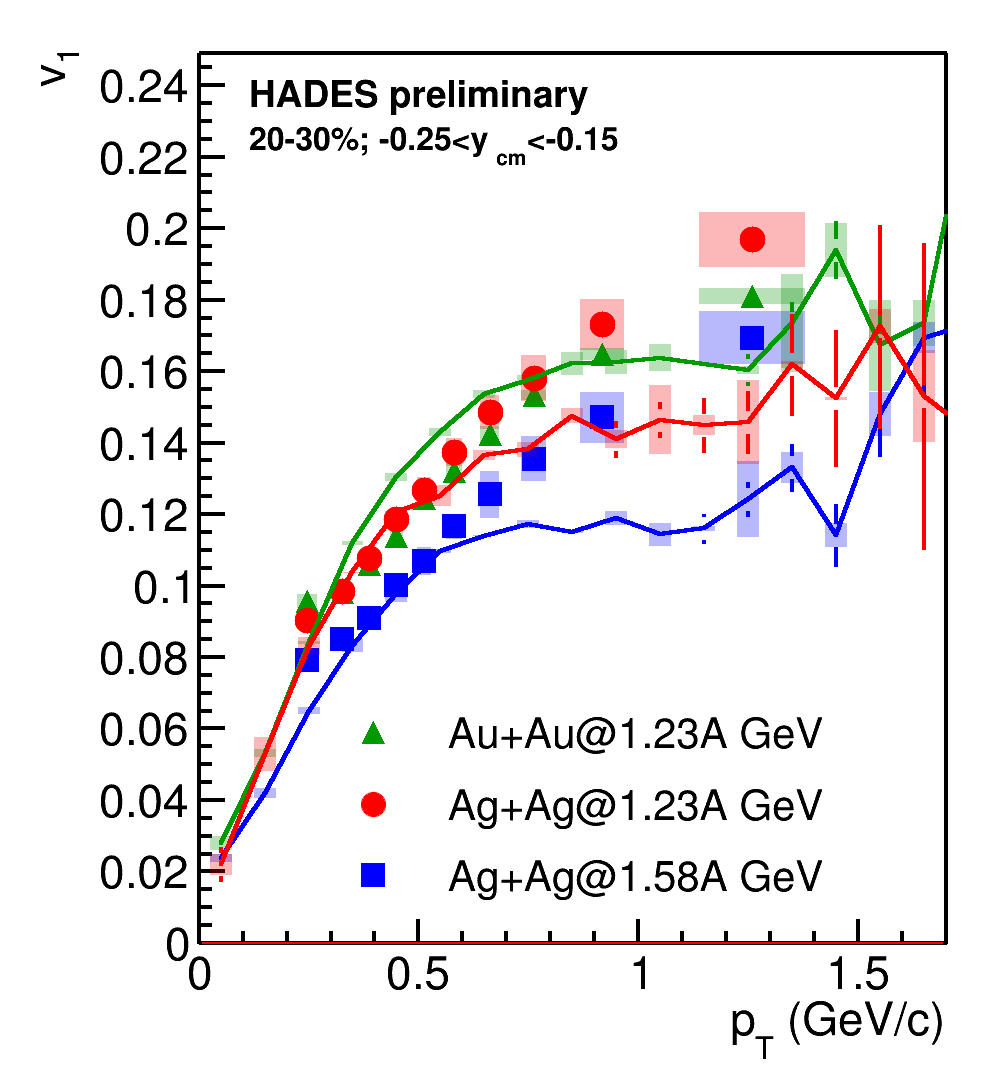
\includegraphics[width=0.45\linewidth]{images/v1_hades_pT.png}
\caption{Направленный поток протонов $v_1$ как фукция (справа) быстроты в системе центра масс $y_{cm}$ и (слева) поперечного импульса $p_T$ для столкновений Au+Au при энергии $E_{kin}=$1.23$A$~ГэВ и Ag+Ag при энергиях $E_{kin}=$1.23$A$ и 1.58$A$~ГэВ. Линиями показаны данные, полученные из модели JAM с импульсно-зависимым потенциалом.}
\label{fig:hades_v1_ycm_pT}
\end{center}
\end{figure}

\subsection{Проверка теоретических предсказаний эффектов масштабирования $v_1$ протнов в реалистичной модели Jet A-A Model (JAM)}

На рис.~\ref{fig:hades_model_ycm_scaling} представлены теоретические предсказания значений направленного потока протонов $v_1$ как функция быстроты столкновения $y_{cm}$ (слева) и быстроты, нормированной на быстроту пучка $y'=y_{cm}/y_{beam}$ (справа) из модели JAM.
Результаты для различных систем при одной энергии столкновения хорошо согласуются между собой и с экспериментальными данными для $v_1$ в столкновениях Au + Au при энергии $E_{kin}$=1.23$A$~ГэВ.
После нормировки быстроты столкновения на быстроту пучка, результаты можно описать единой кривой.
Этот факт свидетельствует о едином механизме образования направленного потока в данной области энергии в тяжелых системах.
%
\begin{figure}[ht]
\begin{center}
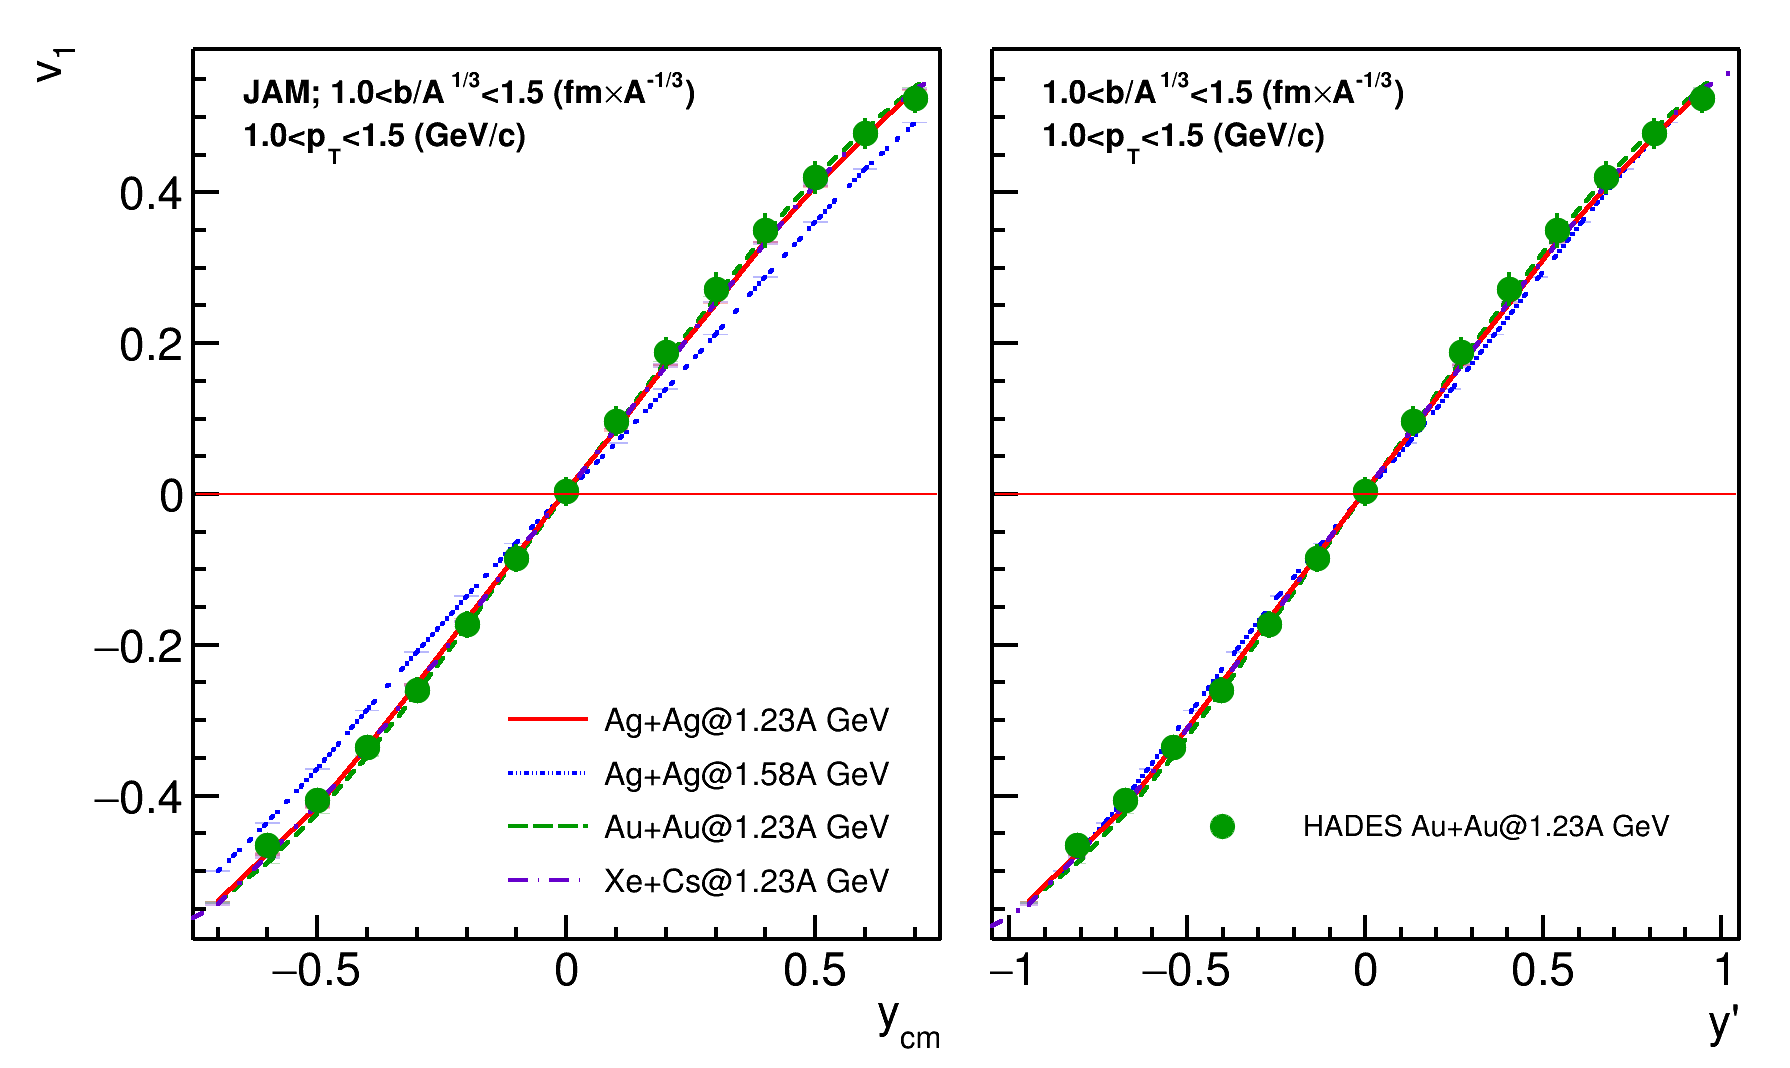
\includegraphics[width=0.95\linewidth]{images/v1_hades_model_ycm_scaling.png}
\caption{Направленный поток протонов $v_1$ как функция быстроты столкновения $y_{cm}$ (слева) и быстроты, нормированной на быстроту пучка $y'=y_{cm}/y_{beam}$ (справа) из модели JAM.}
\label{fig:hades_model_ycm_scaling}
\end{center}
\end{figure}

\subsection{Проверка эффектов масштабирования наклона направленного потока протонов в средних быстротах $dv_1/dy|_{y=0}$}

Зависимость направленного потока протонов $v_1$ как функция быстроты была параметризована кубической функцией $v_1(y_{cm}) = a_0 + a_1 y_{cm} + a_3 y_{cm}^3$. 
Затем наклон направленного потока протонов в нуле быстроты $dv_1/dy_{cm}|_{y_{cm}=0}$ был извлечен как параметр $a_1$.
На рис.~\ref{fig:hades_dv1dy_many_plot} слева приведена зависимость наклона направленного потока в нуле быстроты как функция центральности столкновения.
Наклоны $dv_1/dy_{cm}|_{y_{cm}=0}$ протонов для столкновений Au+Au и Ag+Ag при одной энергии хорошо согласуются между собой за исключением наиболее центральных событий. 
Поскольку при большей энергии время пролета двух ионов меньше, наклон направленного потока протонов в столкновениях Ag+Ag при энергии $E_{kin}=$1.58$A$~ГэВ заметно меньше.
Для коррекции на время пролета, наклон направленного потока протонов $dv_1/dy_{cm}|_{y_{cm}=0}$ был нормирован на быстроту пучка $dv_1/dy_{cm}|_{y_{cm}=0} \times y_{b} = dv_1/dy'|_{y'=0}$, где $y_{b}$ --- быстрота пучка (0.74 для $E_{kin}=$1.23$A$~ГэВ и 0.82 для  $E_{kin}=$1.58$A$~ГэВ) и $y'=y_{cm}/y_b$.
Наклон направленного потока протонов нормированный на быстроту $dv_1/dy'|_{y'=0}$ пучка как функция центральности показан на рис.~\ref{fig:hades_dv1dy_many_plot} в центре. 
За исключением наиболее центральных событий, зависимость наклона от центральности описывается одной кривой для всех трех наборов данных.
В каждом классе центральности был вычислен средний прицельный параметр $\langle b \rangle$. 
Радиус ядра пропорционален корню кубическому из массового числа $r_N \propto A^{1/3}$.
Для устранения зависимости от размера сталкиваемых ядер, средний прицельный параметр в классе центральности был нормирован на $A^{1/3}$.
Наклон направленного потока протонов, нормированный на быстроту пучка $dv_1/dy'|_{y'=0}$ как функция относительного прицельного параметра  $ \langle b \rangle / A^{1/3}$ представлен на рис~\ref{fig:hades_dv1dy_many_plot} справа.
Данное преобразование улучшило согласие зависимостей наклона в центральных событиях. 
%
\begin{figure}[ht]
\begin{center}
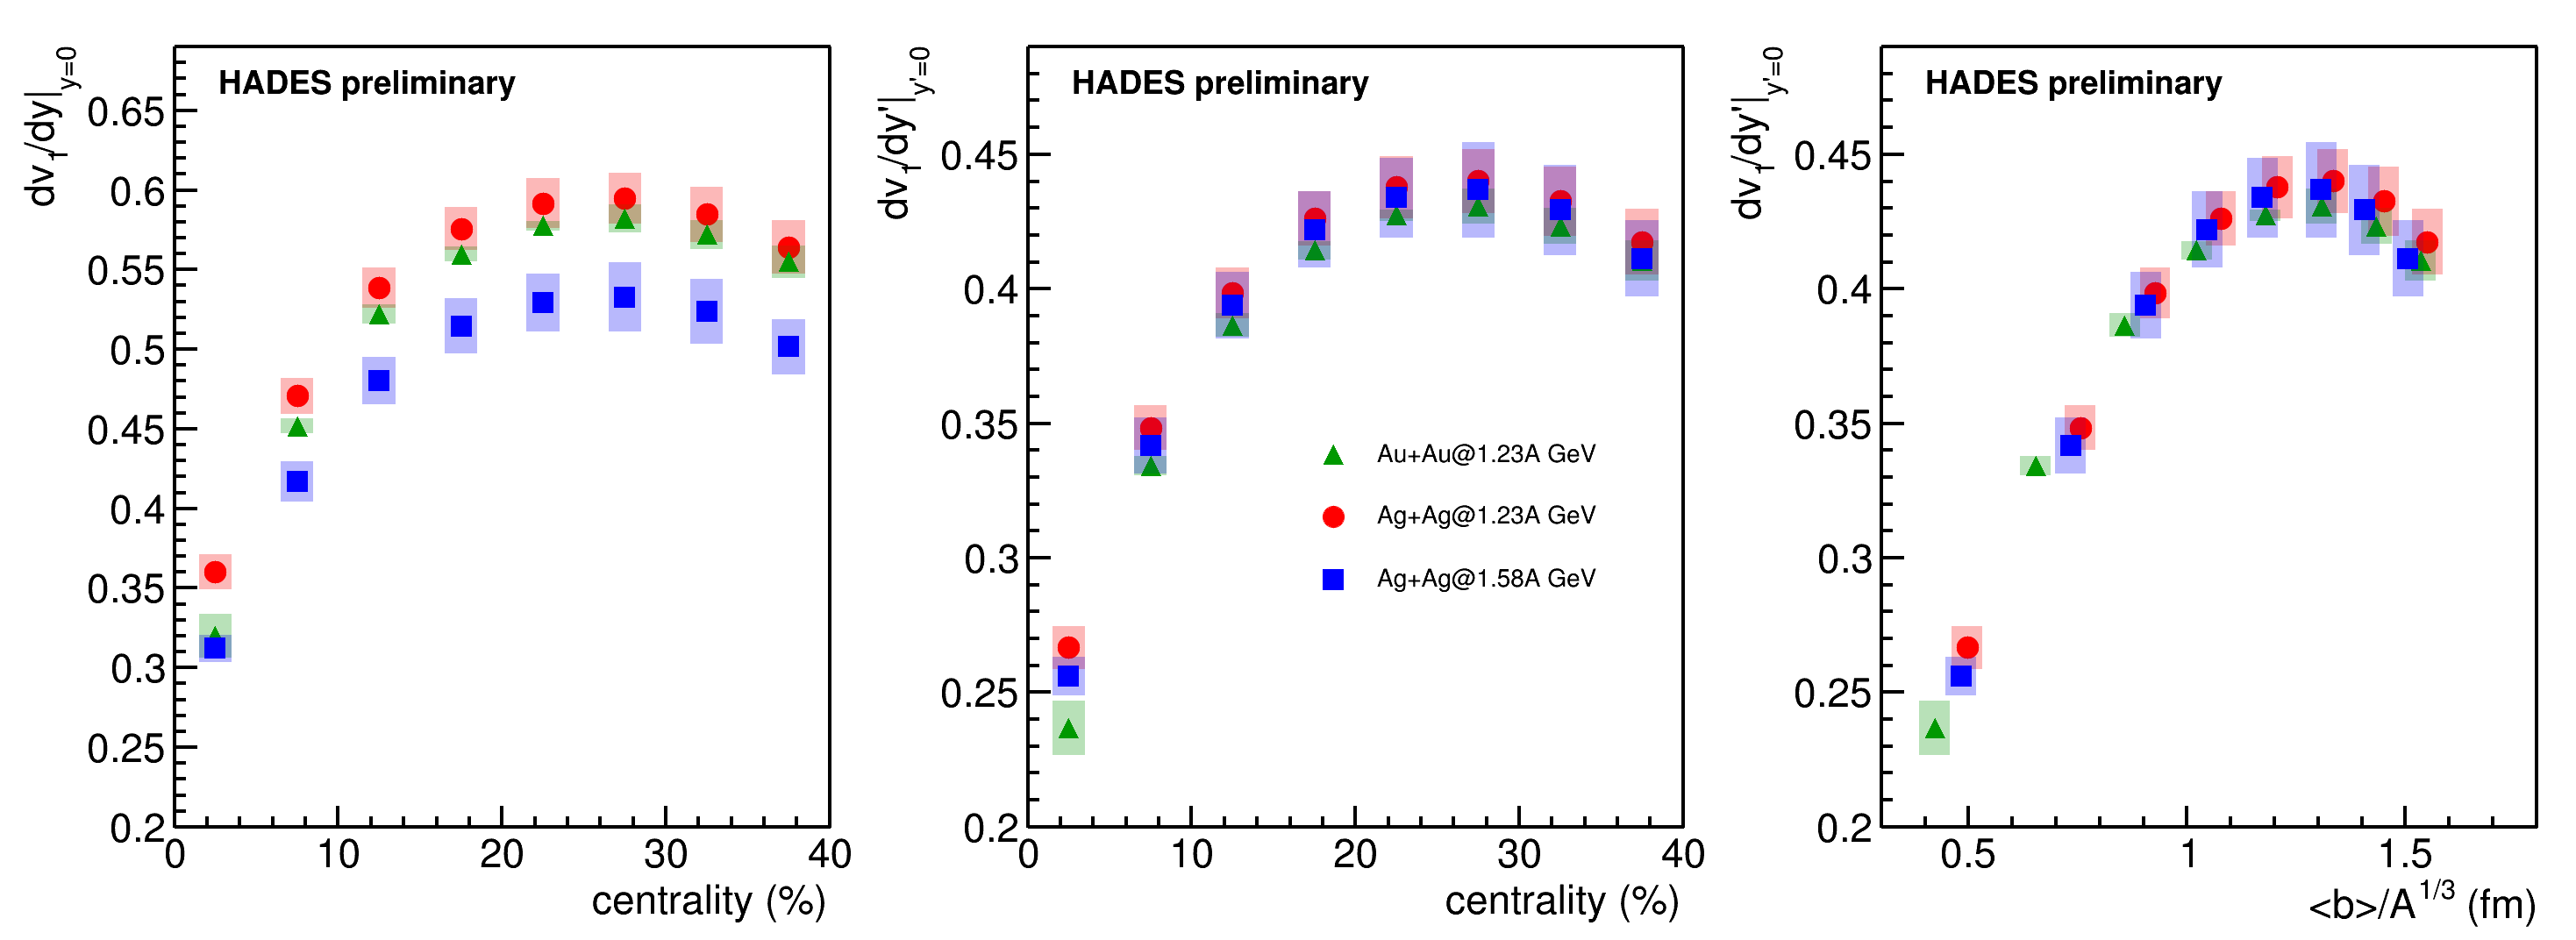
\includegraphics[width=0.9\linewidth]{images/dv1dy_many_plot.png}
\caption{ 
(Слева) Наклон направленного потока в нуле быстроты $dv_1/dy|_{y_{cm}=0}$ как функция центральности столкновений;
(посередине) наклон направленного потока в нуле быстроты нормированный на быстроту пучка $dv_1/dy|_{y'=0}$ как функция центральности столкновений;
(справа) наклон направленного потока в нуле быстроты нормированный на быстроту пучка $dv_1/dy|_{y'=0}$ как функция среднего прицельного параметра в классах центральности
для столкновений Au+Au при энергии $E_{kin}=$1.23$A$~ГэВ и Ag+Ag при энергиях $E_{kin}=$1.23$A$ и 1.58$A$~ГэВ. }
\label{fig:hades_dv1dy_many_plot}
\end{center}
\end{figure}

\subsection{Эффекты масштабирования для направленного потока $v_1$ протонов как функция поперечного импульса}

На рис.~\ref{fig:v1_pT_scaling} представлена зависимость от поперечного импульса $p_T$ направленного потока $v_1$ (слева) и направленного потока, нормированного на наклон в средних быстротах $v_1/dv_1/dy|_{y=0}$ (справа).
Результаты до нормировки для столкновений Au + Au и Ag + Ag при одной энергии находятся в хорошем согласии с учетом систематической ошибки.
Результаты для столкновений Ag + Ag при большей энергии систематически ниже, поскольку величина направленного потока $v_1$ зависит от времени пролета сталкивающихся ядер $t_{pass}$, которая меньше при более высокой энергии.
После нормировки (см. справа), все результаты ложатся на единую кривую.
Этот факт может свидетельствовать о едином механизме образования направленного потока в этой области энергии.
\begin{figure}[ht]
\begin{center}
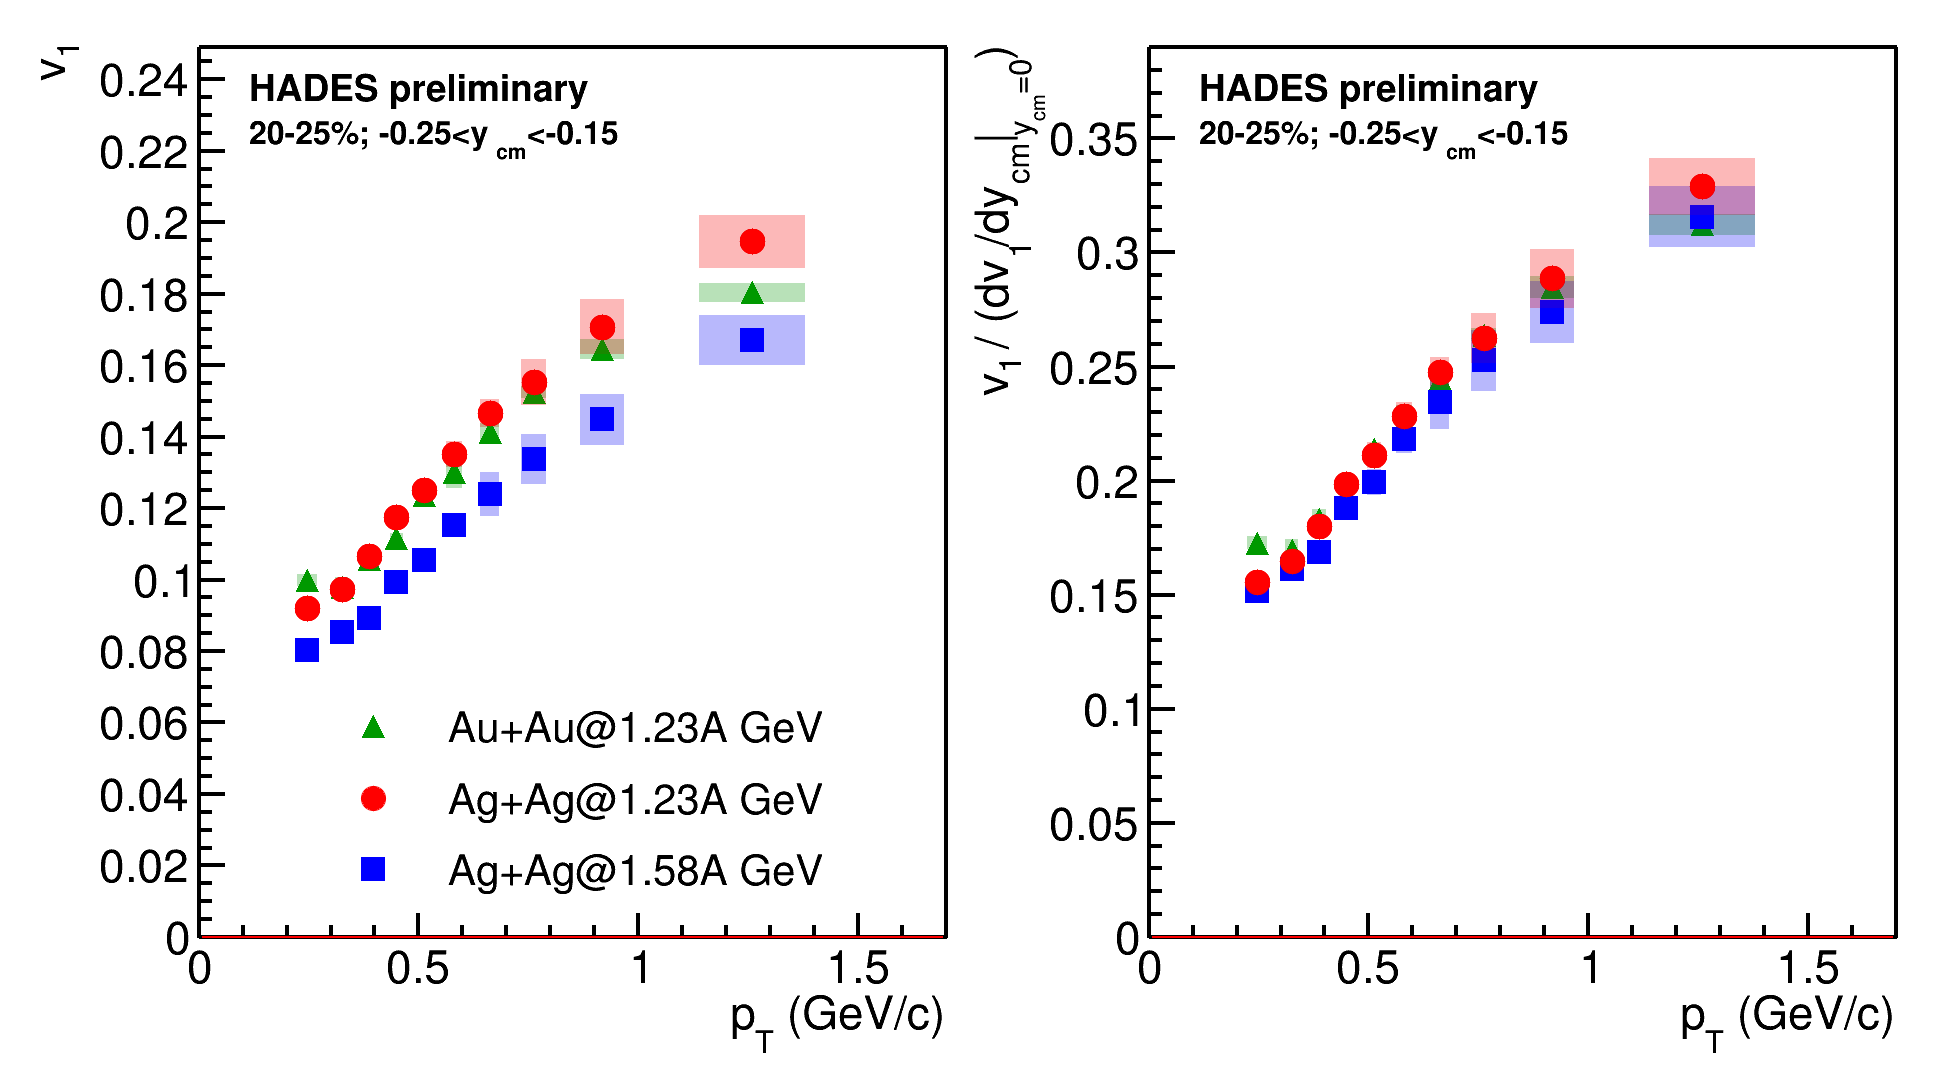
\includegraphics[width=0.9\linewidth]{images/v1_hades_pT_scaling.png}
\caption{ 
    Направленный поток протонов $v_1$ как функция поперечного импульса $p_T$. Слева: направленный поток $v_1$, справа: направленный поток, нормированный на наклон в средних быстротах $v_1/dv_1/dy|_{y=0}$.
}.
\label{fig:v1_pT_scaling}
\end{center}
\end{figure}

Описанный выше эффект был также обнаружен в модели с импульсно-зависимым потенциалом JAM.
На рис.~\ref{fig:v1_model_pT_scaling} представлена зависимость от поперечного импульса $p_T$ направленного потока $v_1$ (слева) и направленного потока, нормированного на наклон в средних быстротах $v_1/dv_1/dy|_{y=0}$ (справа) для различных систем из модели JAM.
До нормировки результаты для направленного потока как функция $p_T$ для столкновений при одной энергии так же находятся в довольно хорошем согласии.
После нормировки, теоретические предсказания так же ложатся на единую кривую. 
\begin{figure}[ht]
\begin{center}
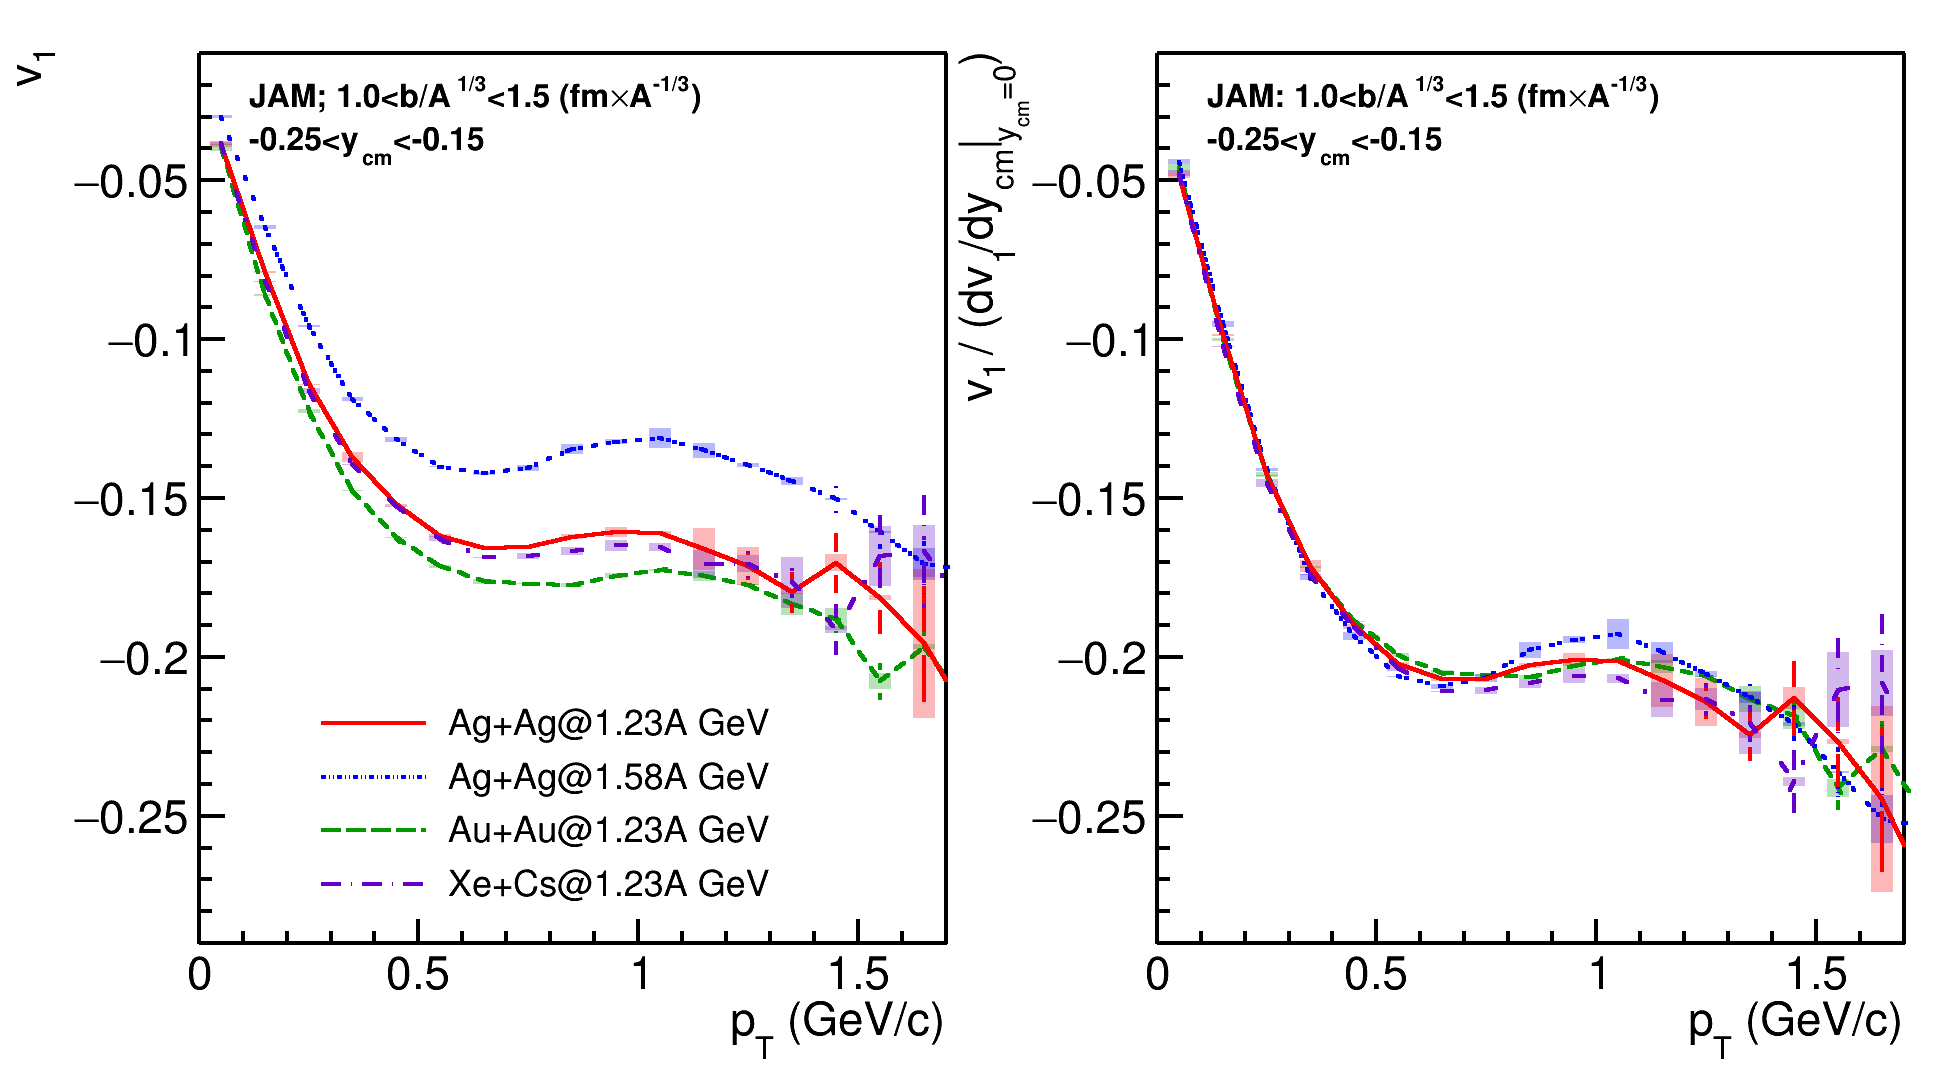
\includegraphics[width=0.9\linewidth]{images/v1_hades_model_pT_scaling.png}
\caption{ 
    Направленный поток протонов $v_1$ как функция поперечного импульса $p_T$ в модели JAM для различных сталкиваемых систем. Слева: направленный поток $v_1$, справа: направленный поток, нормированный на наклон в средних быстротах $v_1/dv_1/dy|_{y=0}$.
}.
\label{fig:v1_model_pT_scaling}
\end{center}
\end{figure}

\subsection{Сравнение измеренного наклона направленного потока протонов в средних быстротах с мировыми данными}

Сравнение полученных значений наклона направленного потока протонов $dv_1/dy|_{y_{cm}=0}$ с существующими результатами показано на рис.~\ref{fig:hades_dv1_dy_sqrt_snn}.
Значения $dv_1/dy|_{y_{cm}=0}$ протонов в столкновениях \au{} при $E_{kin}=$1.23$A$~ГэВ и \ag{} при $E_{kin}=$1.23$A$ и  при $E_{kin}=$1.58$A$~ГэВ согласуются с измерениями с ранее доступными данными с других экспериментов.
%
\begin{figure}[ht]
\begin{center}
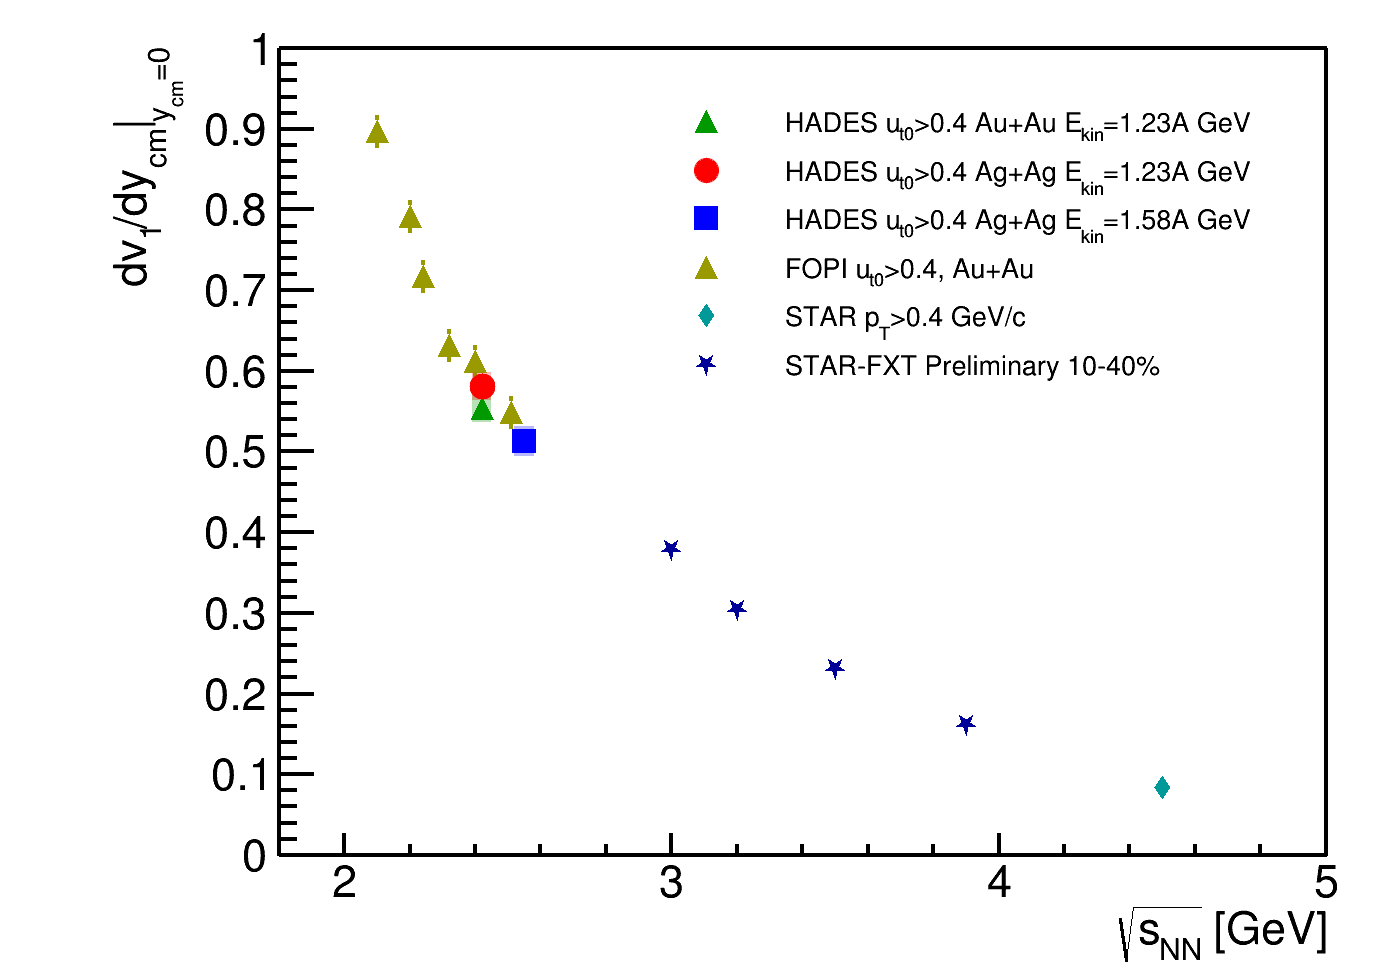
\includegraphics[width=0.9\linewidth]{images/dv1_dy_sqrt_snn.png}
\caption{ 
    Направленный поток протонов $dv_1/dy|_{y_{cm}=0}$ как функция энергии столкновения $\sqrt{s_{NN}}$. Экспериментальные значения наклона направленного потоа были взяты из следующих публикаций: E895~\cite{E895:2000maf}, FOPI~\cite{FOPI:2011aa}, STAR~\cite{STAR:2020dav}.
}
\label{fig:hades_dv1_dy_sqrt_snn}
\end{center}
\end{figure}

\section{Результаты анализа Монте-Карло моделирования эксперимента BM@N}

\subsection{Коррекция на азимутальную неоднородность аксептанса установки}

Эффект применения коррекций на азимутальную неоднородность детектора представлен на рис~\ref{fig:bmn_components}.
%
\begin{figure}[ht]
\begin{center}
\includegraphics[width=0.45\linewidth]{images/v1_proton_correction_rapidity.png}
\caption{Сравнение направленного потока $v_1$ протонов рожденных в Монте-Карло моделировании столкновений Xe+Cs в эксперименте BM@N. Направленный поток получен с использованием различных компонент $u_1$-вектора. Разными маркерами обозначены результаты до и после коррекции на азимутальную неоднородность аксептанса детектора. }
\label{fig:bmn_components}
\end{center}
\end{figure}

Результаты получены для реалистичного моделирования отклика детектора с использованием программного пакета GEANT4.
Разными цветами обозначен результат $v_1$ протонов, полученный с использованием различных компонент $u_1$-вектора. 
Маркеры обозначают результаты до и после коррекции на азимутальную неоднородность детектора.
Черной линией обозначена зависимость $v_1$ протонов извлеченная напрямую из модели без реконструкции.
После применения 3 ступеней коррекции, результаты полученные при помощи $YY$ корреляции $u_1$ и $Q_1$-векторов, хорошо согласуются с результатами извлеченными напрямую из модели.
Напротив, $v_1$, посчитанный с использованием $XX$-компонент, расходится с модельной зависимостью $v_1$ от быстроты. 
Причиной может служить отклонение частиц в направлении оси $x$ в магнитном поле. 
В связи с этим, в дальнейшем для анализа будет использованы лишь корреляции $YY$-компонент $u_1$ и $Q_1$-векторов.

\subsection{Вычисление разрешения плоскости симметрии}

На рис.~\ref{fig:bmn_combinations} представлено разрешение плоскости симметрий $F1$, $F2$, $F3$ (слева направо). 
Аналогично, разрешение посчитанное с использованием комбинаций, не разделенных по быстроте $Q_1$-векторов (к примеру, $F1(F2,F3)$), отличается от значений рассчитанных при помощи комбинаций со значительным разделением по быстроте (к примеру, $F1(Tp,F3)$).
Значения $R_1$, полученные при помощи разделенных по быстроте комбинаций, согласуются между собой в пределах статистической ошибки для всех трех плоскостей симметрии. 
Значительное отличие разрешений, полученных с использованием комбинаций не разделенных по быстроте $Q_1$-векторов, может быть объяснено распространением адронного ливня в поперечном направлении, что вызывает дополнительные корреляции между векторами $F1$ и $F2$, и $F1$ и $F3$.
%
\begin{figure}[ht]
\begin{center}
\includegraphics[width=0.95\linewidth]{images/R1_F123_combinations_centrality.png}
\caption{Разрешение плоскостей симметрии слева: $F1$, посередине: $F2$, справа: $F3$. Различные маркеры и цвета обозначают комбинации $Q_1$-векторов, использованных для расчета разрешения плоскости симметрии.}
\label{fig:bmn_combinations}
\end{center}
\end{figure}

\subsection{Исследование возможности измерения направленного и эллиптического потоков в эксперименте BM@N}

На рис.~\ref{fig:bmn_v1_v2} слева представлен направленный поток протонов, как функция быстроты в Монте-Карло моделировании столкновений $Xe+Cs$ из модели JAM. 
На рис.~\ref{fig:bmn_v1_v2} справа показан эллиптический поток протонов, как функция поперечного импульса в Монте-Карло моделировании столкновений $Xe+Cs$ из модели JAM. 
Разными цветами обозначена разная энергия столкновений. 
Линии обозначают $v_1$ и $v_2$ извлеченные напрямую из модели без реконструкции. 
Маркерами обозначены результаты анализа Монте-Карло моделирования отклика детектора.
Между данными извлеченными из модели и результатами анализа после реалистичной цепочки реконструкции наблюдается согласие в пределах статистической ошибки. 
%
\begin{figure}[ht]
\begin{center}
\includegraphics[width=0.45\linewidth]{images/v1_proton_tof_rapidity.png}
\includegraphics[width=0.45\linewidth]{images/v2_proton_tof_pT.png}
\caption{ 
    Направленный (слева) и эллиптический (справа) поток протонов как функция быстроты и поперечного импульса соответственно в Монте-Карло моделировании столкновений $Xe+Cs$ из модели JAM. Разными цветами обозначена разная энергия столкновений. Линии обозначают $v_1$ и $v_2$ извлеченные напрямую из модели без реконструкции. Маркерами обозначены результаты анализа Монте-Карло моделирования отклика детектора.
}
\label{fig:bmn_v1_v2}
\end{center}
\end{figure}

\section{Выводы к главе 4}
В главе приводятся результаты измерения направленного потока в столкновениях Au+Au при энергии 1.23$A$~ГэВ и Ag+Ag при энергиях 1.23 и 1.58$A$~ГэВ в эксперименте HADES.
Результаты для $v_1$ протонов согласуются с опубликованными коллаборацией HADES.
В главе приводится детальное описание процесса вычисления систематической ошибки, связанной с непотоковыми корреляциями, включенными в финальный опубликованный результат~\cite{HADES:2020lob}.
Произведено сравнение методов вычисления $v_1$: методов плоскости события и скалярного произведения и систематическая разница оказалась в пределах статистической ошибки.
Сравнение направленного потока протонов, измеренных при помощи метода случайных и метода трех подсобытий показывает систматическую разницу порядка 5\% для среднецентральных столкновений ядер Au+Au.
Использование метода случайных подсобытий для вычисления $v_1$ протонов в столкновениях ядер Ag+Ag даёт большую систематическую ошибку, которая может достигать 15\%.
На основании этих оценок, была вычислена систематическая ошибка на измеренные значения коллективных потоков протонов, включенная в публикацию~\cite{HADES:2020lob}.
В главе обсуждаются свойства масштабирования направленного потока протонов $v_1$ с энергией столкновений и размером системы.
Обнаружено, что направленный поток протонов не зависит от энергии столкновений и размера системы в столкновениях Au+Au при энергии 1.23$A$~ГэВ и Ag+Ag при энергиях 1.23 и 1.58$A$~ГэВ в эксперименте HADES.
Значения наклона направленного потока $dv_1/dy$ после коррекции на размер системы и быстроту пучка описываются универсальной зависимостью от относительного прицельного параметра.
Наклон направленного потока $dv_1/dy$ в столкновениях Au+Au при энергии 1.23$A$~ГэВ и Ag+Ag при энергиях 1.23 и 1.58$A$~ГэВ в эксперименте HADES хорошо согласуется с мировыми данными.
В главе представлены результаты исследования Монте-Карло моделирования эксперимента BM@N на возможность измерения направленного и эллиптического потока в первом физическом сеансе установки.
Используя методы, апробированные на экспериментальных данных набранных на установке HADES, была разработа физическая программа измерения коллективной анизотропии в эксперименте BM@N.           % Глава 4
\chapter*{Заключение}						% Заголовок
\addcontentsline{toc}{chapter}{Заключение}	% Добавляем его в оглавление

%% Согласно ГОСТ Р 7.0.11-2011:
%% 5.3.3 В заключении диссертации излагают итоги выполненного исследования, рекомендации, перспективы дальнейшей разработки темы.
%% 9.2.3 В заключении автореферата диссертации излагают итоги данного исследования, рекомендации и перспективы дальнейшей разработки темы.
%% Поэтому имеет смысл сделать эту часть общей и загрузить из одного файла в автореферат и в диссертацию:

Основные результаты работы заключаются в следующем.
%% Согласно ГОСТ Р 7.0.11-2011:
%% 5.3.3 В заключении диссертации излагают итоги выполненного исследования, рекомендации, перспективы дальнейшей разработки темы.
%% 9.2.3 В заключении автореферата диссертации излагают итоги данного исследования, рекомендации и перспективы дальнейшей разработки темы.
\begin{enumerate}
  \item Разработан метод учета корреляций не связанных с коллективным
движением рожденных частиц (непотоковых корреляций) и изучено
их влияние на результаты измерения коллективных потоков в области энергий 1.2-4 АГэВ. 
  \item Впервые получены зависимости  $v_1$ протонов от быстроты и поперечного импульса, а так же наклона $dv_1/dy_{cm}|_{y_{cm}}$ в 
  области средних быстрот в столкновениях \au{} при  энергии  $E_{kin}=$1.23$A$~ГэВ и \ag{} 
  при энергиях $E_{kin}=$1.23$A$ и $E_{kin}=$1.58$A$~ГэВ в эксперименте HADES. Полу­ченные новые результаты измерения $v_1$ протонов современными методами 
  анализа являются принципиально важными для проверки и
дальнейшего развития теоретических моделей ядро-ядерных столкновений.
  \item Обнаружено масштабирование направленного потока протонов с временем пролета ядер $t_{pass}$ и геометрией столкновения в области
   энергий $E_{kin}=$1.23$A$ и $E_{kin}=$1.58$A$~ГэВ, что позволяет оценить влияние спектаторов налетающего ядра на
формирование направленного потока протонов.
  \item На основе моделирования установки детально изучены возможности измерения коллективных потоков протонов на экспериментальной установке BM@N на ускорителе
NUCLOTRON-NICA (ОИЯИ, Дубна). Это позволо расширить существующую физическую программу эксперимента BM@N.
\end{enumerate}

      % Заключение
\chapter*{Список сокращений и условных обозначений}             % Заголовок
\addcontentsline{toc}{chapter}{Список сокращений и условных обозначений}  % Добавляем его в оглавление

\textbf{КЭН} - Кандидат экономических наук

\textbf{РАН} - Российская академия наук

\textbf{РИТЭГ} - Радиоизотопный термоэлектрический генератор

\textbf{PDF} - Portable Document Format
        % Список сокращений и условных обозначений
\chapter*{Словарь терминов}             % Заголовок
\addcontentsline{toc}{chapter}{Словарь терминов}  % Добавляем его в оглавление

\textbf{TeX} - Cистема компьютерной вёрстки, разработанная американским профессором информатики Дональдом Кнутом

\textbf{Панграмма} - Короткий текст, использующий все или почти все буквы алфавита
      % Словарь терминов
\clearpage                                  % В том числе гарантирует, что список литературы в оглавлении будет с правильным номером страницы
\phantomsection
\addcontentsline{toc}{chapter}{\bibname}	% Добавляем список литературы в оглавление
%\hypersetup{ urlcolor=black }               % Ссылки делаем чёрными
%\providecommand*{\BibDash}{}                % В стилях ugost2008 отключаем использование тире как разделителя 
\urlstyle{rm}                               % ссылки URL обычным шрифтом
\insertbibliofull                          % Подключаем Bib-базы
\urlstyle{tt}                               % возвращаем установки шрифта ссылок URL
%\hypersetup{ urlcolor={urlcolor} }          % Восстанавливаем цвет ссылок      % Список литературы
\clearpage
\phantomsection
\addcontentsline{toc}{chapter}{\listfigurename}
\listoffigures									% Список изображений


%%% Список таблиц %%%
% (ГОСТ Р 7.0.11-2011, 5.3.10)
\clearpage
\phantomsection
\addcontentsline{toc}{chapter}{\listtablename}
\listoftables									% Список таблиц
\newpage           % Списки таблиц и изображений (иллюстративный материал)
% \appendix
%% Правка оформления ссылок на приложения:
%http://tex.stackexchange.com/questions/56839/chaptername-is-used-even-for-appendix-chapters-in-toc
%http://tex.stackexchange.com/questions/59349/table-of-contents-with-chapter-and-appendix
%% требует двойной компиляции
\addtocontents{toc}{\def\protect\cftchappresnum{\appendixname{} }%
\setlength{\cftchapnumwidth}{\widthof{\cftchapfont\appendixname~Ш\cftchapaftersnum}}%
}
%% Оформление заголовков приложений ближе к ГОСТ:
\sectionformat{\chapter}[display]{% Параметры заголовков разделов в тексте
    label=\chaptertitlename\ \thechapter,% (ГОСТ Р 2.105, 4.3.6)
    labelsep=20pt,
}
\renewcommand\thechapter{\Asbuk{chapter}} % Чтобы приложения русскими буквами нумеровались
   % Предварительные настройки для правильного подключения Приложений
\chapter{Примеры вставки листингов программного кода} \label{AppendixA}

Для крупных листингов есть два способа. Первый красивый, но в нём могут быть проблемы с поддержкой кириллицы (у вас может встречаться в комментариях и
печатаемых сообщениях), он представлен на листинге~\ref{list:hwbeauty}.
%\renewcommand\FBbskip{-20pt} % если хотим притянуть что-то к плавающему окружению из floatrow
\begin{ListingEnv}[H]% буква H означает Here, ставим здесь,
    % элементы, которые нежелательно разрывать обычно не ставят
    % посреди страницы: вместо H используется t (top, сверху страницы),
    % или b (bottom) или p (page, на отдельной странице)
%    \captionsetup{format=tablenocaption}% должен стоять до самого caption
%    \thisfloatsetup{\capposition=top}%
    \caption{Программа “Hello, world” на \protect\cpp}
    % далее метка для ссылки:
    \label{list:hwbeauty}
    % окружение учитывает пробелы и табляции и приеняет их в сответсвии с настройкми
    \begin{lstlisting}[language={[ISO]C++}]
	#include <iostream>
	using namespace std;

	int main() //кириллица в комментариях при xelatex и lualatex имеет проблемы с пробелами
	{
		cout << "Hello, world" << endl; //latin letters in commentaries
		system("pause");
		return 0;
	}
    \end{lstlisting}
\end{ListingEnv}%
Второй не такой красивый, но без ограничений (см.~листинг~\ref{list:hwplain}).
\begin{ListingEnv}[H]
    \begin{Verb}
        
        #include <iostream>
        using namespace std;
        
        int main() //кириллица в комментариях
        {
            cout << "Привет, мир" << endl;
        }
    \end{Verb}
    \caption{Программа “Hello, world” без подсветки}
    \label{list:hwplain}
\end{ListingEnv}

Можно использовать первый для вставки небольших фрагментов
внутри текста, а второй для вставки полного
кода в приложении, если таковое имеется.

Если нужно вставить совсем короткий пример кода (одна или две строки), то выделение  линейками и нумерация может смотреться чересчур громоздко. В таких случаях можно использовать окружения \texttt{lstlisting} или \texttt{Verb} без \texttt{ListingEnv}. Приведём такой пример с указанием языка программирования, отличного от заданного по умолчанию:
\begin{lstlisting}[language=Haskell]
fibs = 0 : 1 : zipWith (+) fibs (tail fibs)
\end{lstlisting}
Такое решение~--- со вставкой нумерованных листингов покрупнее
и вставок без выделения для маленьких фрагментов~--- выбрано,
например, в книге Эндрю Таненбаума и Тодда Остина по архитектуре
%компьютера~\autocite{TanAus2013} (см.~рис.~\ref{fig:tan-aus}).

Наконец, для оформления идентификаторов внутри строк
(функция \lstinline{main} и тому подобное) используется
\texttt{lstinline} или, самое простое, моноширинный текст
(\texttt{\textbackslash texttt}).


Пример~\ref{list:internal3}, иллюстрирующий подключение переопределённого языка. Может быть полезным, если подсветка кода работает криво. Без дополнительного окружения, с подписью и ссылкой, реализованной встроенным средством.
\begin{lstlisting}[language={Renhanced},caption={Пример листинга c подписью собственными средствами},label={list:internal3}]
## Caching the Inverse of a Matrix

## Matrix inversion is usually a costly computation and there may be some
## benefit to caching the inverse of a matrix rather than compute it repeatedly
## This is a pair of functions that cache the inverse of a matrix.

## makeCacheMatrix creates a special "matrix" object that can cache its inverse

makeCacheMatrix <- function(x = matrix()) {#кириллица в комментариях при xelatex и lualatex имеет проблемы с пробелами
    i <- NULL
    set <- function(y) {
        x <<- y
        i <<- NULL
    }
    get <- function() x
    setSolved <- function(solve) i <<- solve
    getSolved <- function() i
    list(set = set, get = get,
    setSolved = setSolved,
    getSolved = getSolved)
    
}


## cacheSolve computes the inverse of the special "matrix" returned by
## makeCacheMatrix above. If the inverse has already been calculated (and the
## matrix has not changed), then the cachesolve should retrieve the inverse from
## the cache.

cacheSolve <- function(x, ...) {
    ## Return a matrix that is the inverse of 'x'
    i <- x$getSolved()
    if(!is.null(i)) {
        message("getting cached data")
        return(i)
    }
    data <- x$get()
    i <- solve(data, ...)
    x$setSolved(i)
    i  
}
\end{lstlisting} %$ %Комментарий для корректной подсветки синтаксиса
                 %вне листинга

Листинг~\ref{list:external1} подгружается из внешнего файла. Приходится загружать без окружения дополнительного. Иначе по страницам не переносится.
    \lstinputlisting[lastline=78,language={R},caption={Листинг из внешнего файла},label={list:external1}]{listings/run_analysis.R}






\chapter{Очень длинное название второго приложения, в котором продемонстрирована работа с длинными таблицами} \label{AppendixB}

 \section{Подраздел приложения}\label{AppendixB1}
Вот размещается длинная таблица:
\fontsize{10pt}{10pt}\selectfont
\begin{longtable}[c]{|l|c|l|l|}
% \caption{Описание входных файлов модели}\label{Namelists} 
%\\ 
 \hline
 %\multicolumn{4}{|c|}{\textbf{Файл puma\_namelist}}        \\ \hline
 Параметр & Умолч. & Тип & Описание               \\ \hline
                                              \endfirsthead   \hline
 \multicolumn{4}{|c|}{\small\slshape (продолжение)}        \\ \hline
 Параметр & Умолч. & Тип & Описание               \\ \hline
                                              \endhead        \hline
% \multicolumn{4}{|c|}{\small\slshape (окончание)}        \\ \hline
% Параметр & Умолч. & Тип & Описание               \\ \hline
%                                             \endlasthead        \hline
 \multicolumn{4}{|r|}{\small\slshape продолжение следует}  \\ \hline
                                              \endfoot        \hline
                                              \endlastfoot
 \multicolumn{4}{|l|}{\&INP}        \\ \hline 
 kick & 1 & int & 0: инициализация без шума ($p_s = const$) \\
      &   &     & 1: генерация белого шума                  \\
      &   &     & 2: генерация белого шума симметрично относительно \\
  & & & экватора    \\
 mars & 0 & int & 1: инициализация модели для планеты Марс     \\
 kick & 1 & int & 0: инициализация без шума ($p_s = const$) \\
      &   &     & 1: генерация белого шума                  \\
      &   &     & 2: генерация белого шума симметрично относительно \\
  & & & экватора    \\
 mars & 0 & int & 1: инициализация модели для планеты Марс     \\
kick & 1 & int & 0: инициализация без шума ($p_s = const$) \\
      &   &     & 1: генерация белого шума                  \\
      &   &     & 2: генерация белого шума симметрично относительно \\
  & & & экватора    \\
 mars & 0 & int & 1: инициализация модели для планеты Марс     \\
kick & 1 & int & 0: инициализация без шума ($p_s = const$) \\
      &   &     & 1: генерация белого шума                  \\
      &   &     & 2: генерация белого шума симметрично относительно \\
  & & & экватора    \\
 mars & 0 & int & 1: инициализация модели для планеты Марс     \\
kick & 1 & int & 0: инициализация без шума ($p_s = const$) \\
      &   &     & 1: генерация белого шума                  \\
      &   &     & 2: генерация белого шума симметрично относительно \\
  & & & экватора    \\
 mars & 0 & int & 1: инициализация модели для планеты Марс     \\
kick & 1 & int & 0: инициализация без шума ($p_s = const$) \\
      &   &     & 1: генерация белого шума                  \\
      &   &     & 2: генерация белого шума симметрично относительно \\
  & & & экватора    \\
 mars & 0 & int & 1: инициализация модели для планеты Марс     \\
kick & 1 & int & 0: инициализация без шума ($p_s = const$) \\
      &   &     & 1: генерация белого шума                  \\
      &   &     & 2: генерация белого шума симметрично относительно \\
  & & & экватора    \\
 mars & 0 & int & 1: инициализация модели для планеты Марс     \\
kick & 1 & int & 0: инициализация без шума ($p_s = const$) \\
      &   &     & 1: генерация белого шума                  \\
      &   &     & 2: генерация белого шума симметрично относительно \\
  & & & экватора    \\
 mars & 0 & int & 1: инициализация модели для планеты Марс     \\
kick & 1 & int & 0: инициализация без шума ($p_s = const$) \\
      &   &     & 1: генерация белого шума                  \\
      &   &     & 2: генерация белого шума симметрично относительно \\
  & & & экватора    \\
 mars & 0 & int & 1: инициализация модели для планеты Марс     \\
kick & 1 & int & 0: инициализация без шума ($p_s = const$) \\
      &   &     & 1: генерация белого шума                  \\
      &   &     & 2: генерация белого шума симметрично относительно \\
  & & & экватора    \\
 mars & 0 & int & 1: инициализация модели для планеты Марс     \\
kick & 1 & int & 0: инициализация без шума ($p_s = const$) \\
      &   &     & 1: генерация белого шума                  \\
      &   &     & 2: генерация белого шума симметрично относительно \\
  & & & экватора    \\
 mars & 0 & int & 1: инициализация модели для планеты Марс     \\
kick & 1 & int & 0: инициализация без шума ($p_s = const$) \\
      &   &     & 1: генерация белого шума                  \\
      &   &     & 2: генерация белого шума симметрично относительно \\
  & & & экватора    \\
 mars & 0 & int & 1: инициализация модели для планеты Марс     \\
kick & 1 & int & 0: инициализация без шума ($p_s = const$) \\
      &   &     & 1: генерация белого шума                  \\
      &   &     & 2: генерация белого шума симметрично относительно \\
  & & & экватора    \\
 mars & 0 & int & 1: инициализация модели для планеты Марс     \\
kick & 1 & int & 0: инициализация без шума ($p_s = const$) \\
      &   &     & 1: генерация белого шума                  \\
      &   &     & 2: генерация белого шума симметрично относительно \\
  & & & экватора    \\
 mars & 0 & int & 1: инициализация модели для планеты Марс     \\
kick & 1 & int & 0: инициализация без шума ($p_s = const$) \\
      &   &     & 1: генерация белого шума                  \\
      &   &     & 2: генерация белого шума симметрично относительно \\
  & & & экватора    \\
 mars & 0 & int & 1: инициализация модели для планеты Марс     \\
 \hline
  %& & & $\:$ \\ 
 \multicolumn{4}{|l|}{\&SURFPAR}        \\ \hline
kick & 1 & int & 0: инициализация без шума ($p_s = const$) \\
      &   &     & 1: генерация белого шума                  \\
      &   &     & 2: генерация белого шума симметрично относительно \\
  & & & экватора    \\
 mars & 0 & int & 1: инициализация модели для планеты Марс     \\
kick & 1 & int & 0: инициализация без шума ($p_s = const$) \\
      &   &     & 1: генерация белого шума                  \\
      &   &     & 2: генерация белого шума симметрично относительно \\
  & & & экватора    \\
 mars & 0 & int & 1: инициализация модели для планеты Марс     \\
kick & 1 & int & 0: инициализация без шума ($p_s = const$) \\
      &   &     & 1: генерация белого шума                  \\
      &   &     & 2: генерация белого шума симметрично относительно \\
  & & & экватора    \\
 mars & 0 & int & 1: инициализация модели для планеты Марс     \\
kick & 1 & int & 0: инициализация без шума ($p_s = const$) \\
      &   &     & 1: генерация белого шума                  \\
      &   &     & 2: генерация белого шума симметрично относительно \\
  & & & экватора    \\
 mars & 0 & int & 1: инициализация модели для планеты Марс     \\
kick & 1 & int & 0: инициализация без шума ($p_s = const$) \\
      &   &     & 1: генерация белого шума                  \\
      &   &     & 2: генерация белого шума симметрично относительно \\
  & & & экватора    \\
 mars & 0 & int & 1: инициализация модели для планеты Марс     \\
kick & 1 & int & 0: инициализация без шума ($p_s = const$) \\
      &   &     & 1: генерация белого шума                  \\
      &   &     & 2: генерация белого шума симметрично относительно \\
  & & & экватора    \\
 mars & 0 & int & 1: инициализация модели для планеты Марс     \\
kick & 1 & int & 0: инициализация без шума ($p_s = const$) \\
      &   &     & 1: генерация белого шума                  \\
      &   &     & 2: генерация белого шума симметрично относительно \\
  & & & экватора    \\
 mars & 0 & int & 1: инициализация модели для планеты Марс     \\
kick & 1 & int & 0: инициализация без шума ($p_s = const$) \\
      &   &     & 1: генерация белого шума                  \\
      &   &     & 2: генерация белого шума симметрично относительно \\
  & & & экватора    \\
 mars & 0 & int & 1: инициализация модели для планеты Марс     \\
kick & 1 & int & 0: инициализация без шума ($p_s = const$) \\
      &   &     & 1: генерация белого шума                  \\
      &   &     & 2: генерация белого шума симметрично относительно \\
  & & & экватора    \\
 mars & 0 & int & 1: инициализация модели для планеты Марс     \\ 
 \hline 
\end{longtable}

\normalsize% возвращаем шрифт к нормальному
\section{Ещё один подраздел приложения} \label{AppendixB2}

Нужно больше подразделов приложения!

Пример длинной таблицы с записью продолжения по ГОСТ 2.105

    \centering
	\small
    \begin{longtable}[c]{|l|c|l|l|}
	\caption{Наименование таблицы средней длины}%
    \label{tbl:test5}% label всегда желательно идти после caption
    \\
    \hline
     %\multicolumn{4}{|c|}{\textbf{Файл puma\_namelist}}        \\ \hline
     Параметр & Умолч. & Тип & Описание\\ \hline
     \endfirsthead%
%     \multicolumn{4}{|c|}{\small\slshape (продолжение)}        \\ \hline
 \captionsetup{format=tablenocaption,labelformat=continued}% должен стоять до самого caption
    \caption[]{}\\
    \hline
     Параметр & Умолч. & Тип & Описание\\ \hline
      \endhead
      \hline
%     \multicolumn{4}{|r|}{\small\slshape продолжение следует}  \\
%\hline
     \endfoot
         \hline
     \endlastfoot
     \multicolumn{4}{|l|}{\&INP}        \\ \hline 
     kick & 1 & int & 0: инициализация без шума ($p_s = const$) \\
          &   &     & 1: генерация белого шума                  \\
          &   &     & 2: генерация белого шума симметрично относительно \\
      & & & экватора    \\
     mars & 0 & int & 1: инициализация модели для планеты Марс     \\
     kick & 1 & int & 0: инициализация без шума ($p_s = const$) \\
          &   &     & 1: генерация белого шума                  \\
          &   &     & 2: генерация белого шума симметрично относительно \\
      & & & экватора    \\
     mars & 0 & int & 1: инициализация модели для планеты Марс     \\
    kick & 1 & int & 0: инициализация без шума ($p_s = const$) \\
          &   &     & 1: генерация белого шума                  \\
          &   &     & 2: генерация белого шума симметрично относительно \\
      & & & экватора    \\
     mars & 0 & int & 1: инициализация модели для планеты Марс     \\
    kick & 1 & int & 0: инициализация без шума ($p_s = const$) \\
          &   &     & 1: генерация белого шума                  \\
          &   &     & 2: генерация белого шума симметрично относительно \\
      & & & экватора    \\
     mars & 0 & int & 1: инициализация модели для планеты Марс     \\
    kick & 1 & int & 0: инициализация без шума ($p_s = const$) \\
          &   &     & 1: генерация белого шума                  \\
          &   &     & 2: генерация белого шума симметрично относительно \\
      & & & экватора    \\
     mars & 0 & int & 1: инициализация модели для планеты Марс     \\
    kick & 1 & int & 0: инициализация без шума ($p_s = const$) \\
          &   &     & 1: генерация белого шума                  \\
          &   &     & 2: генерация белого шума симметрично относительно \\
      & & & экватора    \\
     mars & 0 & int & 1: инициализация модели для планеты Марс     \\
    kick & 1 & int & 0: инициализация без шума ($p_s = const$) \\
          &   &     & 1: генерация белого шума                  \\
          &   &     & 2: генерация белого шума симметрично относительно \\
      & & & экватора    \\
     mars & 0 & int & 1: инициализация модели для планеты Марс     \\
    kick & 1 & int & 0: инициализация без шума ($p_s = const$) \\
          &   &     & 1: генерация белого шума                  \\
          &   &     & 2: генерация белого шума симметрично относительно \\
      & & & экватора    \\
     mars & 0 & int & 1: инициализация модели для планеты Марс     \\
    kick & 1 & int & 0: инициализация без шума ($p_s = const$) \\
          &   &     & 1: генерация белого шума                  \\
          &   &     & 2: генерация белого шума симметрично относительно \\
      & & & экватора    \\
     mars & 0 & int & 1: инициализация модели для планеты Марс     \\
    kick & 1 & int & 0: инициализация без шума ($p_s = const$) \\
          &   &     & 1: генерация белого шума                  \\
          &   &     & 2: генерация белого шума симметрично относительно \\
      & & & экватора    \\
     mars & 0 & int & 1: инициализация модели для планеты Марс     \\
    kick & 1 & int & 0: инициализация без шума ($p_s = const$) \\
          &   &     & 1: генерация белого шума                  \\
          &   &     & 2: генерация белого шума симметрично относительно \\
      & & & экватора    \\
     mars & 0 & int & 1: инициализация модели для планеты Марс     \\
    kick & 1 & int & 0: инициализация без шума ($p_s = const$) \\
          &   &     & 1: генерация белого шума                  \\
          &   &     & 2: генерация белого шума симметрично относительно \\
      & & & экватора    \\
     mars & 0 & int & 1: инициализация модели для планеты Марс     \\
    kick & 1 & int & 0: инициализация без шума ($p_s = const$) \\
          &   &     & 1: генерация белого шума                  \\
          &   &     & 2: генерация белого шума симметрично относительно \\
      & & & экватора    \\
     mars & 0 & int & 1: инициализация модели для планеты Марс     \\
    kick & 1 & int & 0: инициализация без шума ($p_s = const$) \\
          &   &     & 1: генерация белого шума                  \\
          &   &     & 2: генерация белого шума симметрично относительно \\
      & & & экватора    \\
     mars & 0 & int & 1: инициализация модели для планеты Марс     \\
    kick & 1 & int & 0: инициализация без шума ($p_s = const$) \\
          &   &     & 1: генерация белого шума                  \\
          &   &     & 2: генерация белого шума симметрично относительно \\
      & & & экватора    \\
     mars & 0 & int & 1: инициализация модели для планеты Марс     \\
     \hline
      %& & & $\:$ \\ 
     \multicolumn{4}{|l|}{\&SURFPAR}        \\ \hline
    kick & 1 & int & 0: инициализация без шума ($p_s = const$) \\
          &   &     & 1: генерация белого шума                  \\
          &   &     & 2: генерация белого шума симметрично относительно \\
      & & & экватора    \\
     mars & 0 & int & 1: инициализация модели для планеты Марс     \\
    kick & 1 & int & 0: инициализация без шума ($p_s = const$) \\
          &   &     & 1: генерация белого шума                  \\
          &   &     & 2: генерация белого шума симметрично относительно \\
      & & & экватора    \\
     mars & 0 & int & 1: инициализация модели для планеты Марс     \\
    kick & 1 & int & 0: инициализация без шума ($p_s = const$) \\
          &   &     & 1: генерация белого шума                  \\
          &   &     & 2: генерация белого шума симметрично относительно \\
      & & & экватора    \\
     mars & 0 & int & 1: инициализация модели для планеты Марс     \\
    kick & 1 & int & 0: инициализация без шума ($p_s = const$) \\
          &   &     & 1: генерация белого шума                  \\
          &   &     & 2: генерация белого шума симметрично относительно \\
      & & & экватора    \\
     mars & 0 & int & 1: инициализация модели для планеты Марс     \\
    kick & 1 & int & 0: инициализация без шума ($p_s = const$) \\
          &   &     & 1: генерация белого шума                  \\
          &   &     & 2: генерация белого шума симметрично относительно \\
      & & & экватора    \\
     mars & 0 & int & 1: инициализация модели для планеты Марс     \\
    kick & 1 & int & 0: инициализация без шума ($p_s = const$) \\
          &   &     & 1: генерация белого шума                  \\
          &   &     & 2: генерация белого шума симметрично относительно \\
      & & & экватора    \\
     mars & 0 & int & 1: инициализация модели для планеты Марс     \\
    kick & 1 & int & 0: инициализация без шума ($p_s = const$) \\
          &   &     & 1: генерация белого шума                  \\
          &   &     & 2: генерация белого шума симметрично относительно \\
      & & & экватора    \\
     mars & 0 & int & 1: инициализация модели для планеты Марс     \\
    kick & 1 & int & 0: инициализация без шума ($p_s = const$) \\
          &   &     & 1: генерация белого шума                  \\
          &   &     & 2: генерация белого шума симметрично относительно \\
      & & & экватора    \\
     mars & 0 & int & 1: инициализация модели для планеты Марс     \\
    kick & 1 & int & 0: инициализация без шума ($p_s = const$) \\
          &   &     & 1: генерация белого шума                  \\
          &   &     & 2: генерация белого шума симметрично относительно \\
      & & & экватора    \\
     mars & 0 & int & 1: инициализация модели для планеты Марс     \\ 
%     \hline 
    \end{longtable}
\normalsize% возвращаем шрифт к нормальному
\section{Очередной подраздел приложения} \label{AppendixB3}

Нужно больше подразделов приложения!

\section{И ещё один подраздел приложения} \label{AppendixB4}

Нужно больше подразделов приложения!

        % Приложения

\end{document}
